%*************************************************************************
% A Classic Thesis Style
% An Homage to The Elements of Typographic Style
%
% Copyright (C) 2017 André Miede and Ivo Pletikosić
%
% If you like the style then I would appreciate a postcard. My address
% can be found in the file ClassicThesis.pdf. A collection of the
% postcards I received so far is available online at
% http://postcards.miede.de
%
% License:
% This program is free software; you can redistribute it and/or modify
% it under the terms of the GNU General Public License as published by
% the Free Software Foundation; either version 2 of the License, or
% (at your option) any later version.
%
% This program is distributed in the hope that it will be useful,
% but WITHOUT ANY WARRANTY; without even the implied warranty of
% MERCHANTABILITY or FITNESS FOR A PARTICULAR PURPOSE.  See the
% GNU General Public License for more details.
%
% You should have received a copy of the GNU General Public License
% along with this program; see the file COPYING.  If not, write to
% the Free Software Foundation, Inc., 59 Temple Place - Suite 330,
% Boston, MA 02111-1307, USA.
%
% PLEASE SEE ALSO THE AUTHORS' NOTE REGARDING THIS LICENSE
% IN THE DOCUMENTATION (ClassicThesis.pdf --> Chapter 1 / Chapter01.tex)
%*************************************************************************
\RequirePackage{silence} % :-\
    \WarningFilter{scrreprt}{Usage of package `titlesec'}
    %\WarningFilter{scrreprt}{Activating an ugly workaround}
    \WarningFilter{titlesec}{Non standard sectioning command detected}
\documentclass[ openright,titlepage,numbers=noenddot,headinclude,%twoside, %1headlines,% letterpaper a4paper
                footinclude=true,cleardoublepage=empty,abstractoff, % <--- obsolete, remove (todo)
                BCOR=5mm,paper=a4,fontsize=11pt,%11pt,a4paper,%
                ngerman,american,%lockflag%
                ]{scrreprt}

%*************************************************************************
% Note: Make all your adjustments in here
%*************************************************************************
% ****************************************************************************************************
% ferniunithesis-config.tex 
% Use it at the beginning of your thesis.tex, or as a LaTeX Preamble 
% in your thesis.{tex,lyx} with \input{fernunithesis-config}
% ****************************************************************************************************

% ****************************************************************************************************
% 1. Personal data and user ad-hoc commands
% ****************************************************************************************************
\newcommand{\myTitle}{Data Science Storytelling für Kraftfahrzeug-basierte Daten\xspace}
%\newcommand{\mySubtitle}{An Homage to The Elements of Typographic Style\xspace}
\newcommand{\myDegree}{Master of Science (M.Sc.)\xspace} 
\newcommand{\myThesisType}{Masterarbeit\xspace}
\newcommand{\myName}{Jasmin Sophia Kraft\xspace}
\newcommand{\myId}{3981630\xspace}
\newcommand{\myProf}{Univ.-Prof. Dr. Christian Beecks\xspace}
\newcommand{\secondProf}{Dr. Simone Opel\xspace}
\newcommand{\referent}{Prüfer\xspace}% Referentin/Referent, depending on the gender of your prof
\newcommand{\secondReferent}{Zweitprüfer\xspace}% Referentin/Referent, depending on the gender of your prof
\newcommand{\mySupervisor}{Andrea Linxen\xspace}
\newcommand{\supervisor}{Betreuerin\xspace}% Betreuerin/Betreuer, depending on the gender of your supervisor
\newcommand{\myFaculty}{Fakult\"at f\"ur Mathematik und Informatik\xspace}
\newcommand{\myUni}{FernUniversit\"at in Hagen\xspace}
\newcommand{\mySubjectArea}{Lehrgebiet Data Science\xspace}
\newcommand{\myLocation}{Kempten (Allgäu)\xspace}
\newcommand{\myTime}{05. Mai 2024\xspace}
\newcommand{\myVersion}{version 4.4\xspace}

% ****************************************************************************************************
% 2. Is it a master thesis?
% ****************************************************************************************************
\PassOptionsToPackage{master}{fernunihesis} % uncomment if this is a master thesis 

% ****************************************************************************************************
% 3. Does the thesis have a lock flag?
% ****************************************************************************************************
\PassOptionsToPackage{lockflag}{fernunithesis} % uncomment if this thesis has a lock flag 

% ****************************************************************************************************
% 4. Loading some handy packages
% ****************************************************************************************************
% ****************************************************************************************************
% Packages with options that might require adjustments
% ****************************************************************************************************

%\PassOptionsToPackage{ngerman,american}{babel}   % change this to your language(s)
% Spanish languages need extra options in order to work with this template
%\PassOptionsToPackage{spanish,es-lcroman}{babel}
\usepackage{babel}


% ****************************************************************************************************
% classicthesis-config.tex
% formerly known as loadpackages.sty, classicthesis-ldpkg.sty, and classicthesis-preamble.sty
% Use it at the beginning of your ClassicThesis.tex, or as a LaTeX Preamble
% in your ClassicThesis.{tex,lyx} with % ****************************************************************************************************
% classicthesis-config.tex
% formerly known as loadpackages.sty, classicthesis-ldpkg.sty, and classicthesis-preamble.sty
% Use it at the beginning of your ClassicThesis.tex, or as a LaTeX Preamble
% in your ClassicThesis.{tex,lyx} with % ****************************************************************************************************
% classicthesis-config.tex
% formerly known as loadpackages.sty, classicthesis-ldpkg.sty, and classicthesis-preamble.sty
% Use it at the beginning of your ClassicThesis.tex, or as a LaTeX Preamble
% in your ClassicThesis.{tex,lyx} with \input{classicthesis-config}
% ****************************************************************************************************
% If you like the classicthesis, then I would appreciate a postcard.
% My address can be found in the file ClassicThesis.pdf. A collection
% of the postcards I received so far is available online at
% http://postcards.miede.de
% ****************************************************************************************************


% ****************************************************************************************************
% 0. Set the encoding of your files. UTF-8 is the only sensible encoding nowadays. If you can't read
% äöüßáéçèê∂åëæƒÏ€ then change the encoding setting in your editor, not the line below. If your editor
% does not support utf8 use another editor!
% ****************************************************************************************************
\PassOptionsToPackage{utf8}{inputenc}
  \usepackage{inputenc}

% ****************************************************************************************************
% 1. Configure classicthesis for your needs here, e.g., remove "drafting" below
% in order to deactivate the time-stamp on the pages
% (see ClassicThesis.pdf for more information):
% ****************************************************************************************************
\PassOptionsToPackage{
  drafting=false,   % print version information on the bottom of the pages
  tocaligned=false, % the left column of the toc will be aligned (no indentation)
  dottedtoc=true,   % page numbers in ToC flushed right
  parts=true,       % use part division
  eulerchapternumbers=true, % use AMS Euler for chapter font (otherwise Palatino)
  linedheaders=false,       % chaper headers will have line above and beneath
  floatperchapter=true,     % numbering per chapter for all floats (i.e., Figure 1.1)
  listings=true,    % load listings package and setup LoL
  subfig=true,      % setup for preloaded subfig package
  eulermath=false,  % use awesome Euler fonts for mathematical formulae (only with pdfLaTeX)
  beramono=true,    % toggle a nice monospaced font (w/ bold)
  minionpro=false   % setup for minion pro font; use minion pro small caps as well (only with pdfLaTeX)
}{classicthesis}


% ****************************************************************************************************
% 2. Personal data and user ad-hoc commands
% ****************************************************************************************************
%\newcommand{\myTitle}{A Classic Thesis Style\xspace}
%\newcommand{\mySubtitle}{An Homage to The Elements of Typographic Style\xspace}
%\newcommand{\myDegree}{Doktor-Ingenieur (Dr.-Ing.)\xspace}
%\newcommand{\myName}{André Miede\xspace}
%\newcommand{\myProf}{Put name here\xspace}
%\newcommand{\myOtherProf}{Put name here\xspace}
%\newcommand{\mySupervisor}{Put name here\xspace}
%\newcommand{\myFaculty}{Put data here\xspace}
%\newcommand{\myDepartment}{Put data here\xspace}
%\newcommand{\myUni}{Put data here\xspace}
%\newcommand{\myLocation}{Saarbrücken\xspace}
%\newcommand{\myTime}{October 2017\xspace}
%\newcommand{\myVersion}{version 4.4}

% ********************************************************************
% Setup, finetuning, and useful commands
% ********************************************************************
\newcounter{dummy} % necessary for correct hyperlinks (to index, bib, etc.)
\newlength{\abcd} % for ab..z string length calculation
\providecommand{\mLyX}{L\kern-.1667em\lower.25em\hbox{Y}\kern-.125emX\@}
\newcommand{\ie}{i.\,e.}
\newcommand{\Ie}{I.\,e.}
\newcommand{\eg}{e.\,g.}
\newcommand{\Eg}{E.\,g.}
% ****************************************************************************************************


% ****************************************************************************************************
% 3. Loading some handy packages
% ****************************************************************************************************
% ********************************************************************
% Packages with options that might require adjustments
% ********************************************************************
%\PassOptionsToPackage{ngerman,american}{babel}   % change this to your language(s), main language last
% Spanish languages need extra options in order to work with this template
%\PassOptionsToPackage{spanish,es-lcroman}{babel}
\usepackage{babel}

\usepackage{csquotes}

\PassOptionsToPackage{%
  %backend=biber,bibencoding=utf8, %instead of bibtex
  backend=bibtex8,bibencoding=ascii,%
  language=auto,%
  %style=numeric-comp,%
  style=alphabetic,%
  %style=authoryear-comp, % Author 1999, 2010
  %bibstyle=authoryear,dashed=false, % dashed: substitute rep. author with ---
  sorting=nyt, % name, year, title
  maxbibnames=10, % default: 3, et al.
  %backref=true,%
  natbib=true % natbib compatibility mode (\citep and \citet still work)
}{biblatex}
  \usepackage{biblatex}

\PassOptionsToPackage{fleqn}{amsmath}       % math environments and more by the AMS
  \usepackage{amsmath}

\PassOptionsToPackage{doublespacing}{fernuni-hagen-thesis}  % options: abbrev exam big wiwi english master
  \usepackage{fernuni-hagen-thesis}

% ********************************************************************
% General useful packages
% ********************************************************************
\PassOptionsToPackage{T1}{fontenc} % T2A for cyrillics
  \usepackage{fontenc}
\usepackage{textcomp} % fix warning with missing font shapes
\usepackage{scrhack} % fix warnings when using KOMA with listings package
\usepackage{xspace} % to get the spacing after macros right
\usepackage{mparhack} % get marginpar right
%\usepackage{fixltx2e} % fixes some LaTeX stuff --> since 2015 in the LaTeX kernel (see below)
% \usepackage[latest]{latexrelease} % emulate newer kernel version if older is detected
\PassOptionsToPackage{printonlyused,smaller}{acronym}
  \usepackage{acronym} % nice macros for handling all acronyms in the thesis
  %\renewcommand{\bflabel}[1]{{#1}\hfill} % fix the list of acronyms --> no longer working
  %\renewcommand*{\acsfont}[1]{\textsc{#1}}
  %\renewcommand*{\aclabelfont}[1]{\acsfont{#1}}
  %\def\bflabel#1{{#1\hfill}}
  \def\bflabel#1{{\acsfont{#1}\hfill}}
  \def\aclabelfont#1{\acsfont{#1}}
% ****************************************************************************************************

% ****************************************************************************************************
% 4. Setup floats: tables, (sub)figures, and captions
% ****************************************************************************************************
\usepackage{tabularx} % better tables
  \setlength{\extrarowheight}{3pt} % increase table row height
\newcommand{\tableheadline}[1]{\multicolumn{1}{c}{\spacedlowsmallcaps{#1}}}
\newcommand{\myfloatalign}{\centering} % to be used with each float for alignment
\usepackage{caption}
% Thanks to cgnieder and Claus Lahiri
% http://tex.stackexchange.com/questions/69349/spacedlowsmallcaps-in-caption-label
% [REMOVED DUE TO OTHER PROBLEMS, SEE ISSUE #82]
%\DeclareCaptionLabelFormat{smallcaps}{\bothIfFirst{#1}{~}\MakeTextLowercase{\textsc{#2}}}
%\captionsetup{font=small,labelformat=smallcaps} % format=hang,
\captionsetup{font=small} % format=hang,
\usepackage{subfig}
% ****************************************************************************************************


% ****************************************************************************************************
% 5. Setup code listings
% ****************************************************************************************************
\usepackage{listings}
%\lstset{emph={trueIndex,root},emphstyle=\color{BlueViolet}}%\underbar} % for special keywords
\lstset{language=[LaTeX]Tex,%C++,
  morekeywords={PassOptionsToPackage,selectlanguage},
  keywordstyle=\color{RoyalBlue},%\bfseries,
  basicstyle=\small\ttfamily,
  %identifierstyle=\color{NavyBlue},
  commentstyle=\color{Green}\ttfamily,
  stringstyle=\rmfamily,
  numbers=none,%left,%
  numberstyle=\scriptsize,%\tiny
  stepnumber=5,
  numbersep=8pt,
  showstringspaces=false,
  breaklines=true,
  %frameround=ftff,
  %frame=single,
  belowcaptionskip=.75\baselineskip
  %frame=L
}
% ****************************************************************************************************


% ****************************************************************************************************
% 6. PDFLaTeX, hyperreferences, and citation backreferences
% ****************************************************************************************************
% ********************************************************************
% Using PDFLaTeX
% ********************************************************************
\PassOptionsToPackage{hyperfootnotes=false,pdfpagelabels}{hyperref}
  \usepackage{hyperref}  % backref linktocpage pagebackref
%\ifpdf
%\pdfcompresslevel=9
%\pdfadjustspacing=1
%\fi
%\PassOptionsToPackage{pdftex}{graphicx} %%%IVO: driver will be chosen automatically
  \usepackage{graphicx}


% ********************************************************************
% Hyperreferences
% ********************************************************************
\hypersetup{%
  %draft, % hyperref's draft mode, for printing see below
  colorlinks=true, linktocpage=true, pdfstartpage=3, pdfstartview=FitV,%
  % uncomment the following line if you want to have black links (e.g., for printing)
  %colorlinks=false, linktocpage=false, pdfstartpage=3, pdfstartview=FitV, pdfborder={0 0 0},%
  breaklinks=true, pdfpagemode=UseNone, pageanchor=true, pdfpagemode=UseOutlines,%
  plainpages=false, bookmarksnumbered, bookmarksopen=true, bookmarksopenlevel=1,%
  hypertexnames=true, pdfhighlight=/O,%nesting=true,%frenchlinks,%
  %urlcolor=webbrown, linkcolor=RoyalBlue, citecolor=webgreen, %pagecolor=RoyalBlue,%
  urlcolor=Black, linkcolor=Black, citecolor=Black, %pagecolor=Black,%
  pdftitle={\myTitle},%
  pdfauthor={\textcopyright\ \myName, \myUni, \myFaculty},%
  pdfsubject={},%
  pdfkeywords={},%
  pdfcreator={pdfLaTeX},%
  pdfproducer={LaTeX with hyperref and classicthesis}%
}

% ********************************************************************
% Setup autoreferences
% ********************************************************************
% There are some issues regarding autorefnames
% http://www.ureader.de/msg/136221647.aspx
% http://www.tex.ac.uk/cgi-bin/texfaq2html?label=latexwords
% you have to redefine the makros for the
% language you use, e.g., american, ngerman
% (as chosen when loading babel/AtBeginDocument)
% ********************************************************************
\makeatletter
\@ifpackageloaded{babel}%
  {%
    \addto\extrasamerican{%
      \renewcommand*{\figureautorefname}{Figure}%
      \renewcommand*{\tableautorefname}{Table}%
      \renewcommand*{\partautorefname}{Part}%
      \renewcommand*{\chapterautorefname}{Chapter}%
      \renewcommand*{\sectionautorefname}{Section}%
      \renewcommand*{\subsectionautorefname}{Section}%
      \renewcommand*{\subsubsectionautorefname}{Section}%
    }%
    \addto\extrasngerman{%
      \renewcommand*{\paragraphautorefname}{Absatz}%
      \renewcommand*{\subparagraphautorefname}{Unterabsatz}%
      \renewcommand*{\footnoteautorefname}{Fu\"snote}%
      \renewcommand*{\FancyVerbLineautorefname}{Zeile}%
      \renewcommand*{\theoremautorefname}{Theorem}%
      \renewcommand*{\appendixautorefname}{Anhang}%
      \renewcommand*{\equationautorefname}{Gleichung}%
      \renewcommand*{\itemautorefname}{Punkt}%
    }%
      % Fix to getting autorefs for subfigures right (thanks to Belinda Vogt for changing the definition)
      \providecommand{\subfigureautorefname}{\figureautorefname}%
    }{\relax}
\makeatother


% ****************************************************************************************************
% 7. Last calls before the bar closes
% ****************************************************************************************************
% ********************************************************************
% Development Stuff
% ********************************************************************
\listfiles
%\PassOptionsToPackage{l2tabu,orthodox,abort}{nag}
%  \usepackage{nag}
%\PassOptionsToPackage{warning, all}{onlyamsmath}
%  \usepackage{onlyamsmath}

% ********************************************************************
% Last, but not least...
% ********************************************************************
\usepackage{classicthesis}
% ****************************************************************************************************


% ****************************************************************************************************
% 8. Further adjustments (experimental)
% ****************************************************************************************************
% ********************************************************************
% Changing the text area
% ********************************************************************
%\areaset[current]{312pt}{761pt} % 686 (factor 2.2) + 33 head + 42 head \the\footskip
%\setlength{\marginparwidth}{7em}%
%\setlength{\marginparsep}{2em}%

% ********************************************************************
% Using different fonts
% ********************************************************************
%\usepackage[oldstylenums]{kpfonts} % oldstyle notextcomp
%\usepackage[osf]{libertine}
%\usepackage[light,condensed,math]{iwona}
%\renewcommand{\sfdefault}{iwona}
%\usepackage{lmodern} % <-- no osf support :-(
%\usepackage{cfr-lm} %
%\usepackage[urw-garamond]{mathdesign} <-- no osf support :-(
%\usepackage[default,osfigures]{opensans} % scale=0.95
%\usepackage[sfdefault]{FiraSans}
% ********************************************************************
% \usepackage[largesc,osf]{newpxtext}
% Used to fix these:
% https://bitbucket.org/amiede/classicthesis/issues/139/italics-in-pallatino-capitals-chapter
% https://bitbucket.org/amiede/classicthesis/issues/45/problema-testatine-su-classicthesis-style
% ********************************************************************
%\linespread{1.05} % a bit more for Palatino
% ****************************************************************************************************

% ****************************************************************************************************
% If you like the classicthesis, then I would appreciate a postcard.
% My address can be found in the file ClassicThesis.pdf. A collection
% of the postcards I received so far is available online at
% http://postcards.miede.de
% ****************************************************************************************************


% ****************************************************************************************************
% 0. Set the encoding of your files. UTF-8 is the only sensible encoding nowadays. If you can't read
% äöüßáéçèê∂åëæƒÏ€ then change the encoding setting in your editor, not the line below. If your editor
% does not support utf8 use another editor!
% ****************************************************************************************************
\PassOptionsToPackage{utf8}{inputenc}
  \usepackage{inputenc}

% ****************************************************************************************************
% 1. Configure classicthesis for your needs here, e.g., remove "drafting" below
% in order to deactivate the time-stamp on the pages
% (see ClassicThesis.pdf for more information):
% ****************************************************************************************************
\PassOptionsToPackage{
  drafting=false,   % print version information on the bottom of the pages
  tocaligned=false, % the left column of the toc will be aligned (no indentation)
  dottedtoc=true,   % page numbers in ToC flushed right
  parts=true,       % use part division
  eulerchapternumbers=true, % use AMS Euler for chapter font (otherwise Palatino)
  linedheaders=false,       % chaper headers will have line above and beneath
  floatperchapter=true,     % numbering per chapter for all floats (i.e., Figure 1.1)
  listings=true,    % load listings package and setup LoL
  subfig=true,      % setup for preloaded subfig package
  eulermath=false,  % use awesome Euler fonts for mathematical formulae (only with pdfLaTeX)
  beramono=true,    % toggle a nice monospaced font (w/ bold)
  minionpro=false   % setup for minion pro font; use minion pro small caps as well (only with pdfLaTeX)
}{classicthesis}


% ****************************************************************************************************
% 2. Personal data and user ad-hoc commands
% ****************************************************************************************************
%\newcommand{\myTitle}{A Classic Thesis Style\xspace}
%\newcommand{\mySubtitle}{An Homage to The Elements of Typographic Style\xspace}
%\newcommand{\myDegree}{Doktor-Ingenieur (Dr.-Ing.)\xspace}
%\newcommand{\myName}{André Miede\xspace}
%\newcommand{\myProf}{Put name here\xspace}
%\newcommand{\myOtherProf}{Put name here\xspace}
%\newcommand{\mySupervisor}{Put name here\xspace}
%\newcommand{\myFaculty}{Put data here\xspace}
%\newcommand{\myDepartment}{Put data here\xspace}
%\newcommand{\myUni}{Put data here\xspace}
%\newcommand{\myLocation}{Saarbrücken\xspace}
%\newcommand{\myTime}{October 2017\xspace}
%\newcommand{\myVersion}{version 4.4}

% ********************************************************************
% Setup, finetuning, and useful commands
% ********************************************************************
\newcounter{dummy} % necessary for correct hyperlinks (to index, bib, etc.)
\newlength{\abcd} % for ab..z string length calculation
\providecommand{\mLyX}{L\kern-.1667em\lower.25em\hbox{Y}\kern-.125emX\@}
\newcommand{\ie}{i.\,e.}
\newcommand{\Ie}{I.\,e.}
\newcommand{\eg}{e.\,g.}
\newcommand{\Eg}{E.\,g.}
% ****************************************************************************************************


% ****************************************************************************************************
% 3. Loading some handy packages
% ****************************************************************************************************
% ********************************************************************
% Packages with options that might require adjustments
% ********************************************************************
%\PassOptionsToPackage{ngerman,american}{babel}   % change this to your language(s), main language last
% Spanish languages need extra options in order to work with this template
%\PassOptionsToPackage{spanish,es-lcroman}{babel}
\usepackage{babel}

\usepackage{csquotes}

\PassOptionsToPackage{%
  %backend=biber,bibencoding=utf8, %instead of bibtex
  backend=bibtex8,bibencoding=ascii,%
  language=auto,%
  %style=numeric-comp,%
  style=alphabetic,%
  %style=authoryear-comp, % Author 1999, 2010
  %bibstyle=authoryear,dashed=false, % dashed: substitute rep. author with ---
  sorting=nyt, % name, year, title
  maxbibnames=10, % default: 3, et al.
  %backref=true,%
  natbib=true % natbib compatibility mode (\citep and \citet still work)
}{biblatex}
  \usepackage{biblatex}

\PassOptionsToPackage{fleqn}{amsmath}       % math environments and more by the AMS
  \usepackage{amsmath}

\PassOptionsToPackage{doublespacing}{fernuni-hagen-thesis}  % options: abbrev exam big wiwi english master
  \usepackage{fernuni-hagen-thesis}

% ********************************************************************
% General useful packages
% ********************************************************************
\PassOptionsToPackage{T1}{fontenc} % T2A for cyrillics
  \usepackage{fontenc}
\usepackage{textcomp} % fix warning with missing font shapes
\usepackage{scrhack} % fix warnings when using KOMA with listings package
\usepackage{xspace} % to get the spacing after macros right
\usepackage{mparhack} % get marginpar right
%\usepackage{fixltx2e} % fixes some LaTeX stuff --> since 2015 in the LaTeX kernel (see below)
% \usepackage[latest]{latexrelease} % emulate newer kernel version if older is detected
\PassOptionsToPackage{printonlyused,smaller}{acronym}
  \usepackage{acronym} % nice macros for handling all acronyms in the thesis
  %\renewcommand{\bflabel}[1]{{#1}\hfill} % fix the list of acronyms --> no longer working
  %\renewcommand*{\acsfont}[1]{\textsc{#1}}
  %\renewcommand*{\aclabelfont}[1]{\acsfont{#1}}
  %\def\bflabel#1{{#1\hfill}}
  \def\bflabel#1{{\acsfont{#1}\hfill}}
  \def\aclabelfont#1{\acsfont{#1}}
% ****************************************************************************************************

% ****************************************************************************************************
% 4. Setup floats: tables, (sub)figures, and captions
% ****************************************************************************************************
\usepackage{tabularx} % better tables
  \setlength{\extrarowheight}{3pt} % increase table row height
\newcommand{\tableheadline}[1]{\multicolumn{1}{c}{\spacedlowsmallcaps{#1}}}
\newcommand{\myfloatalign}{\centering} % to be used with each float for alignment
\usepackage{caption}
% Thanks to cgnieder and Claus Lahiri
% http://tex.stackexchange.com/questions/69349/spacedlowsmallcaps-in-caption-label
% [REMOVED DUE TO OTHER PROBLEMS, SEE ISSUE #82]
%\DeclareCaptionLabelFormat{smallcaps}{\bothIfFirst{#1}{~}\MakeTextLowercase{\textsc{#2}}}
%\captionsetup{font=small,labelformat=smallcaps} % format=hang,
\captionsetup{font=small} % format=hang,
\usepackage{subfig}
% ****************************************************************************************************


% ****************************************************************************************************
% 5. Setup code listings
% ****************************************************************************************************
\usepackage{listings}
%\lstset{emph={trueIndex,root},emphstyle=\color{BlueViolet}}%\underbar} % for special keywords
\lstset{language=[LaTeX]Tex,%C++,
  morekeywords={PassOptionsToPackage,selectlanguage},
  keywordstyle=\color{RoyalBlue},%\bfseries,
  basicstyle=\small\ttfamily,
  %identifierstyle=\color{NavyBlue},
  commentstyle=\color{Green}\ttfamily,
  stringstyle=\rmfamily,
  numbers=none,%left,%
  numberstyle=\scriptsize,%\tiny
  stepnumber=5,
  numbersep=8pt,
  showstringspaces=false,
  breaklines=true,
  %frameround=ftff,
  %frame=single,
  belowcaptionskip=.75\baselineskip
  %frame=L
}
% ****************************************************************************************************


% ****************************************************************************************************
% 6. PDFLaTeX, hyperreferences, and citation backreferences
% ****************************************************************************************************
% ********************************************************************
% Using PDFLaTeX
% ********************************************************************
\PassOptionsToPackage{hyperfootnotes=false,pdfpagelabels}{hyperref}
  \usepackage{hyperref}  % backref linktocpage pagebackref
%\ifpdf
%\pdfcompresslevel=9
%\pdfadjustspacing=1
%\fi
%\PassOptionsToPackage{pdftex}{graphicx} %%%IVO: driver will be chosen automatically
  \usepackage{graphicx}


% ********************************************************************
% Hyperreferences
% ********************************************************************
\hypersetup{%
  %draft, % hyperref's draft mode, for printing see below
  colorlinks=true, linktocpage=true, pdfstartpage=3, pdfstartview=FitV,%
  % uncomment the following line if you want to have black links (e.g., for printing)
  %colorlinks=false, linktocpage=false, pdfstartpage=3, pdfstartview=FitV, pdfborder={0 0 0},%
  breaklinks=true, pdfpagemode=UseNone, pageanchor=true, pdfpagemode=UseOutlines,%
  plainpages=false, bookmarksnumbered, bookmarksopen=true, bookmarksopenlevel=1,%
  hypertexnames=true, pdfhighlight=/O,%nesting=true,%frenchlinks,%
  %urlcolor=webbrown, linkcolor=RoyalBlue, citecolor=webgreen, %pagecolor=RoyalBlue,%
  urlcolor=Black, linkcolor=Black, citecolor=Black, %pagecolor=Black,%
  pdftitle={\myTitle},%
  pdfauthor={\textcopyright\ \myName, \myUni, \myFaculty},%
  pdfsubject={},%
  pdfkeywords={},%
  pdfcreator={pdfLaTeX},%
  pdfproducer={LaTeX with hyperref and classicthesis}%
}

% ********************************************************************
% Setup autoreferences
% ********************************************************************
% There are some issues regarding autorefnames
% http://www.ureader.de/msg/136221647.aspx
% http://www.tex.ac.uk/cgi-bin/texfaq2html?label=latexwords
% you have to redefine the makros for the
% language you use, e.g., american, ngerman
% (as chosen when loading babel/AtBeginDocument)
% ********************************************************************
\makeatletter
\@ifpackageloaded{babel}%
  {%
    \addto\extrasamerican{%
      \renewcommand*{\figureautorefname}{Figure}%
      \renewcommand*{\tableautorefname}{Table}%
      \renewcommand*{\partautorefname}{Part}%
      \renewcommand*{\chapterautorefname}{Chapter}%
      \renewcommand*{\sectionautorefname}{Section}%
      \renewcommand*{\subsectionautorefname}{Section}%
      \renewcommand*{\subsubsectionautorefname}{Section}%
    }%
    \addto\extrasngerman{%
      \renewcommand*{\paragraphautorefname}{Absatz}%
      \renewcommand*{\subparagraphautorefname}{Unterabsatz}%
      \renewcommand*{\footnoteautorefname}{Fu\"snote}%
      \renewcommand*{\FancyVerbLineautorefname}{Zeile}%
      \renewcommand*{\theoremautorefname}{Theorem}%
      \renewcommand*{\appendixautorefname}{Anhang}%
      \renewcommand*{\equationautorefname}{Gleichung}%
      \renewcommand*{\itemautorefname}{Punkt}%
    }%
      % Fix to getting autorefs for subfigures right (thanks to Belinda Vogt for changing the definition)
      \providecommand{\subfigureautorefname}{\figureautorefname}%
    }{\relax}
\makeatother


% ****************************************************************************************************
% 7. Last calls before the bar closes
% ****************************************************************************************************
% ********************************************************************
% Development Stuff
% ********************************************************************
\listfiles
%\PassOptionsToPackage{l2tabu,orthodox,abort}{nag}
%  \usepackage{nag}
%\PassOptionsToPackage{warning, all}{onlyamsmath}
%  \usepackage{onlyamsmath}

% ********************************************************************
% Last, but not least...
% ********************************************************************
\usepackage{classicthesis}
% ****************************************************************************************************


% ****************************************************************************************************
% 8. Further adjustments (experimental)
% ****************************************************************************************************
% ********************************************************************
% Changing the text area
% ********************************************************************
%\areaset[current]{312pt}{761pt} % 686 (factor 2.2) + 33 head + 42 head \the\footskip
%\setlength{\marginparwidth}{7em}%
%\setlength{\marginparsep}{2em}%

% ********************************************************************
% Using different fonts
% ********************************************************************
%\usepackage[oldstylenums]{kpfonts} % oldstyle notextcomp
%\usepackage[osf]{libertine}
%\usepackage[light,condensed,math]{iwona}
%\renewcommand{\sfdefault}{iwona}
%\usepackage{lmodern} % <-- no osf support :-(
%\usepackage{cfr-lm} %
%\usepackage[urw-garamond]{mathdesign} <-- no osf support :-(
%\usepackage[default,osfigures]{opensans} % scale=0.95
%\usepackage[sfdefault]{FiraSans}
% ********************************************************************
% \usepackage[largesc,osf]{newpxtext}
% Used to fix these:
% https://bitbucket.org/amiede/classicthesis/issues/139/italics-in-pallatino-capitals-chapter
% https://bitbucket.org/amiede/classicthesis/issues/45/problema-testatine-su-classicthesis-style
% ********************************************************************
%\linespread{1.05} % a bit more for Palatino
% ****************************************************************************************************

% ****************************************************************************************************
% If you like the classicthesis, then I would appreciate a postcard.
% My address can be found in the file ClassicThesis.pdf. A collection
% of the postcards I received so far is available online at
% http://postcards.miede.de
% ****************************************************************************************************


% ****************************************************************************************************
% 0. Set the encoding of your files. UTF-8 is the only sensible encoding nowadays. If you can't read
% äöüßáéçèê∂åëæƒÏ€ then change the encoding setting in your editor, not the line below. If your editor
% does not support utf8 use another editor!
% ****************************************************************************************************
\PassOptionsToPackage{utf8}{inputenc}
  \usepackage{inputenc}

% ****************************************************************************************************
% 1. Configure classicthesis for your needs here, e.g., remove "drafting" below
% in order to deactivate the time-stamp on the pages
% (see ClassicThesis.pdf for more information):
% ****************************************************************************************************
\PassOptionsToPackage{
  drafting=false,   % print version information on the bottom of the pages
  tocaligned=false, % the left column of the toc will be aligned (no indentation)
  dottedtoc=true,   % page numbers in ToC flushed right
  parts=true,       % use part division
  eulerchapternumbers=true, % use AMS Euler for chapter font (otherwise Palatino)
  linedheaders=false,       % chaper headers will have line above and beneath
  floatperchapter=true,     % numbering per chapter for all floats (i.e., Figure 1.1)
  listings=true,    % load listings package and setup LoL
  subfig=true,      % setup for preloaded subfig package
  eulermath=false,  % use awesome Euler fonts for mathematical formulae (only with pdfLaTeX)
  beramono=true,    % toggle a nice monospaced font (w/ bold)
  minionpro=false   % setup for minion pro font; use minion pro small caps as well (only with pdfLaTeX)
}{classicthesis}


% ****************************************************************************************************
% 2. Personal data and user ad-hoc commands
% ****************************************************************************************************
%\newcommand{\myTitle}{A Classic Thesis Style\xspace}
%\newcommand{\mySubtitle}{An Homage to The Elements of Typographic Style\xspace}
%\newcommand{\myDegree}{Doktor-Ingenieur (Dr.-Ing.)\xspace}
%\newcommand{\myName}{André Miede\xspace}
%\newcommand{\myProf}{Put name here\xspace}
%\newcommand{\myOtherProf}{Put name here\xspace}
%\newcommand{\mySupervisor}{Put name here\xspace}
%\newcommand{\myFaculty}{Put data here\xspace}
%\newcommand{\myDepartment}{Put data here\xspace}
%\newcommand{\myUni}{Put data here\xspace}
%\newcommand{\myLocation}{Saarbrücken\xspace}
%\newcommand{\myTime}{October 2017\xspace}
%\newcommand{\myVersion}{version 4.4}

% ********************************************************************
% Setup, finetuning, and useful commands
% ********************************************************************
\newcounter{dummy} % necessary for correct hyperlinks (to index, bib, etc.)
\newlength{\abcd} % for ab..z string length calculation
\providecommand{\mLyX}{L\kern-.1667em\lower.25em\hbox{Y}\kern-.125emX\@}
\newcommand{\ie}{i.\,e.}
\newcommand{\Ie}{I.\,e.}
\newcommand{\eg}{e.\,g.}
\newcommand{\Eg}{E.\,g.}
% ****************************************************************************************************


% ****************************************************************************************************
% 3. Loading some handy packages
% ****************************************************************************************************
% ********************************************************************
% Packages with options that might require adjustments
% ********************************************************************
%\PassOptionsToPackage{ngerman,american}{babel}   % change this to your language(s), main language last
% Spanish languages need extra options in order to work with this template
%\PassOptionsToPackage{spanish,es-lcroman}{babel}
\usepackage{babel}

\usepackage{csquotes}

\PassOptionsToPackage{%
  %backend=biber,bibencoding=utf8, %instead of bibtex
  backend=bibtex8,bibencoding=ascii,%
  language=auto,%
  %style=numeric-comp,%
  style=alphabetic,%
  %style=authoryear-comp, % Author 1999, 2010
  %bibstyle=authoryear,dashed=false, % dashed: substitute rep. author with ---
  sorting=nyt, % name, year, title
  maxbibnames=10, % default: 3, et al.
  %backref=true,%
  natbib=true % natbib compatibility mode (\citep and \citet still work)
}{biblatex}
  \usepackage{biblatex}

\PassOptionsToPackage{fleqn}{amsmath}       % math environments and more by the AMS
  \usepackage{amsmath}

\PassOptionsToPackage{doublespacing}{fernuni-hagen-thesis}  % options: abbrev exam big wiwi english master
  \usepackage{fernuni-hagen-thesis}

% ********************************************************************
% General useful packages
% ********************************************************************
\PassOptionsToPackage{T1}{fontenc} % T2A for cyrillics
  \usepackage{fontenc}
\usepackage{textcomp} % fix warning with missing font shapes
\usepackage{scrhack} % fix warnings when using KOMA with listings package
\usepackage{xspace} % to get the spacing after macros right
\usepackage{mparhack} % get marginpar right
%\usepackage{fixltx2e} % fixes some LaTeX stuff --> since 2015 in the LaTeX kernel (see below)
% \usepackage[latest]{latexrelease} % emulate newer kernel version if older is detected
\PassOptionsToPackage{printonlyused,smaller}{acronym}
  \usepackage{acronym} % nice macros for handling all acronyms in the thesis
  %\renewcommand{\bflabel}[1]{{#1}\hfill} % fix the list of acronyms --> no longer working
  %\renewcommand*{\acsfont}[1]{\textsc{#1}}
  %\renewcommand*{\aclabelfont}[1]{\acsfont{#1}}
  %\def\bflabel#1{{#1\hfill}}
  \def\bflabel#1{{\acsfont{#1}\hfill}}
  \def\aclabelfont#1{\acsfont{#1}}
% ****************************************************************************************************

% ****************************************************************************************************
% 4. Setup floats: tables, (sub)figures, and captions
% ****************************************************************************************************
\usepackage{tabularx} % better tables
  \setlength{\extrarowheight}{3pt} % increase table row height
\newcommand{\tableheadline}[1]{\multicolumn{1}{c}{\spacedlowsmallcaps{#1}}}
\newcommand{\myfloatalign}{\centering} % to be used with each float for alignment
\usepackage{caption}
% Thanks to cgnieder and Claus Lahiri
% http://tex.stackexchange.com/questions/69349/spacedlowsmallcaps-in-caption-label
% [REMOVED DUE TO OTHER PROBLEMS, SEE ISSUE #82]
%\DeclareCaptionLabelFormat{smallcaps}{\bothIfFirst{#1}{~}\MakeTextLowercase{\textsc{#2}}}
%\captionsetup{font=small,labelformat=smallcaps} % format=hang,
\captionsetup{font=small} % format=hang,
\usepackage{subfig}
% ****************************************************************************************************


% ****************************************************************************************************
% 5. Setup code listings
% ****************************************************************************************************
\usepackage{listings}
%\lstset{emph={trueIndex,root},emphstyle=\color{BlueViolet}}%\underbar} % for special keywords
\lstset{language=[LaTeX]Tex,%C++,
  morekeywords={PassOptionsToPackage,selectlanguage},
  keywordstyle=\color{RoyalBlue},%\bfseries,
  basicstyle=\small\ttfamily,
  %identifierstyle=\color{NavyBlue},
  commentstyle=\color{Green}\ttfamily,
  stringstyle=\rmfamily,
  numbers=none,%left,%
  numberstyle=\scriptsize,%\tiny
  stepnumber=5,
  numbersep=8pt,
  showstringspaces=false,
  breaklines=true,
  %frameround=ftff,
  %frame=single,
  belowcaptionskip=.75\baselineskip
  %frame=L
}
% ****************************************************************************************************


% ****************************************************************************************************
% 6. PDFLaTeX, hyperreferences, and citation backreferences
% ****************************************************************************************************
% ********************************************************************
% Using PDFLaTeX
% ********************************************************************
\PassOptionsToPackage{hyperfootnotes=false,pdfpagelabels}{hyperref}
  \usepackage{hyperref}  % backref linktocpage pagebackref
%\ifpdf
%\pdfcompresslevel=9
%\pdfadjustspacing=1
%\fi
%\PassOptionsToPackage{pdftex}{graphicx} %%%IVO: driver will be chosen automatically
  \usepackage{graphicx}


% ********************************************************************
% Hyperreferences
% ********************************************************************
\hypersetup{%
  %draft, % hyperref's draft mode, for printing see below
  colorlinks=true, linktocpage=true, pdfstartpage=3, pdfstartview=FitV,%
  % uncomment the following line if you want to have black links (e.g., for printing)
  %colorlinks=false, linktocpage=false, pdfstartpage=3, pdfstartview=FitV, pdfborder={0 0 0},%
  breaklinks=true, pdfpagemode=UseNone, pageanchor=true, pdfpagemode=UseOutlines,%
  plainpages=false, bookmarksnumbered, bookmarksopen=true, bookmarksopenlevel=1,%
  hypertexnames=true, pdfhighlight=/O,%nesting=true,%frenchlinks,%
  %urlcolor=webbrown, linkcolor=RoyalBlue, citecolor=webgreen, %pagecolor=RoyalBlue,%
  urlcolor=Black, linkcolor=Black, citecolor=Black, %pagecolor=Black,%
  pdftitle={\myTitle},%
  pdfauthor={\textcopyright\ \myName, \myUni, \myFaculty},%
  pdfsubject={},%
  pdfkeywords={},%
  pdfcreator={pdfLaTeX},%
  pdfproducer={LaTeX with hyperref and classicthesis}%
}

% ********************************************************************
% Setup autoreferences
% ********************************************************************
% There are some issues regarding autorefnames
% http://www.ureader.de/msg/136221647.aspx
% http://www.tex.ac.uk/cgi-bin/texfaq2html?label=latexwords
% you have to redefine the makros for the
% language you use, e.g., american, ngerman
% (as chosen when loading babel/AtBeginDocument)
% ********************************************************************
\makeatletter
\@ifpackageloaded{babel}%
  {%
    \addto\extrasamerican{%
      \renewcommand*{\figureautorefname}{Figure}%
      \renewcommand*{\tableautorefname}{Table}%
      \renewcommand*{\partautorefname}{Part}%
      \renewcommand*{\chapterautorefname}{Chapter}%
      \renewcommand*{\sectionautorefname}{Section}%
      \renewcommand*{\subsectionautorefname}{Section}%
      \renewcommand*{\subsubsectionautorefname}{Section}%
    }%
    \addto\extrasngerman{%
      \renewcommand*{\paragraphautorefname}{Absatz}%
      \renewcommand*{\subparagraphautorefname}{Unterabsatz}%
      \renewcommand*{\footnoteautorefname}{Fu\"snote}%
      \renewcommand*{\FancyVerbLineautorefname}{Zeile}%
      \renewcommand*{\theoremautorefname}{Theorem}%
      \renewcommand*{\appendixautorefname}{Anhang}%
      \renewcommand*{\equationautorefname}{Gleichung}%
      \renewcommand*{\itemautorefname}{Punkt}%
    }%
      % Fix to getting autorefs for subfigures right (thanks to Belinda Vogt for changing the definition)
      \providecommand{\subfigureautorefname}{\figureautorefname}%
    }{\relax}
\makeatother


% ****************************************************************************************************
% 7. Last calls before the bar closes
% ****************************************************************************************************
% ********************************************************************
% Development Stuff
% ********************************************************************
\listfiles
%\PassOptionsToPackage{l2tabu,orthodox,abort}{nag}
%  \usepackage{nag}
%\PassOptionsToPackage{warning, all}{onlyamsmath}
%  \usepackage{onlyamsmath}

% ********************************************************************
% Last, but not least...
% ********************************************************************
\usepackage{classicthesis}
% ****************************************************************************************************


% ****************************************************************************************************
% 8. Further adjustments (experimental)
% ****************************************************************************************************
% ********************************************************************
% Changing the text area
% ********************************************************************
%\areaset[current]{312pt}{761pt} % 686 (factor 2.2) + 33 head + 42 head \the\footskip
%\setlength{\marginparwidth}{7em}%
%\setlength{\marginparsep}{2em}%

% ********************************************************************
% Using different fonts
% ********************************************************************
%\usepackage[oldstylenums]{kpfonts} % oldstyle notextcomp
%\usepackage[osf]{libertine}
%\usepackage[light,condensed,math]{iwona}
%\renewcommand{\sfdefault}{iwona}
%\usepackage{lmodern} % <-- no osf support :-(
%\usepackage{cfr-lm} %
%\usepackage[urw-garamond]{mathdesign} <-- no osf support :-(
%\usepackage[default,osfigures]{opensans} % scale=0.95
%\usepackage[sfdefault]{FiraSans}
% ********************************************************************
% \usepackage[largesc,osf]{newpxtext}
% Used to fix these:
% https://bitbucket.org/amiede/classicthesis/issues/139/italics-in-pallatino-capitals-chapter
% https://bitbucket.org/amiede/classicthesis/issues/45/problema-testatine-su-classicthesis-style
% ********************************************************************
%\linespread{1.05} % a bit more for Palatino
% ****************************************************************************************************


%linenumbers
\usepackage{lineno}
\usepackage{csquotes}
\usepackage{multicol}
\usepackage{hyperref}

\usepackage{parskip}

%code style
\usepackage{xcolor}
\definecolor{lightgray}{rgb}{.9,.9,.9}
\definecolor{darkgray}{rgb}{.4,.4,.4}
\definecolor{purple}{rgb}{0.65, 0.12, 0.82}
\lstdefinelanguage{TypeScript}{
  keywords={break, case, catch, continue, debugger, default, delete, do, else, false, finally, for, function, if, in, instanceof, new, return, switch, this, throw, true, try, typeof, var, void, while, with, readonly, private, public, const, Interface},
  morecomment=[l]{//},
  morecomment=[s]{/*}{*/},
  morestring=[b]',
  morestring=[b]",
  ndkeywords={class, export, boolean, throw, implements, import, this, string, number, any, undefined},
  keywordstyle=\color{blue}\bfseries,
  ndkeywordstyle=\color{darkgray}\bfseries,
  identifierstyle=\color{black},
  commentstyle=\color{purple}\ttfamily,
  stringstyle=\color{red}\ttfamily,
  sensitive=true
}


\lstset{
   language=TypeScript,
   backgroundcolor=\color{lightgray},
   extendedchars=true,
   basicstyle=\footnotesize\ttfamily,
   showstringspaces=false,
   showspaces=false,
   numbers=left,
   numberstyle=\footnotesize,
   numbersep=9pt,
   tabsize=2,
   breaklines=true,
   showtabs=false,
   captionpos=b
}
\newcommand{\llabel}[1]{\hypertarget{llineno:#1}{\linelabel{#1}}}
\newcommand{\lref}[1]{\hyperlink{llineno:#1}{\ref*{#1}}}


%*************************************************************************
% Bibliographies
%*************************************************************************
\addbibresource{quellen.bib}

%*************************************************************************
% Hyphenation
%*************************************************************************
%\hyphenation{put special hyphenation here}

%*************************************************************************
% GO!GO!GO! MOVE IT!
%*************************************************************************
\begin{document}
\frenchspacing
\raggedbottom
\selectlanguage{ngerman} % ngerman, american
%\renewcommand*{\bibname}{new name}
%\setbibpreamble{}
\pagenumbering{roman}
\pagestyle{plain}
%*************************************************************************
% Frontmatter
%*************************************************************************
%*******************************************************
% Titlepage
%*******************************************************
%%%
%%% title page (german)
%%%
\thispagestyle{empty}
\pdfbookmark[0]{Titelblatt}{title}
\begin{titlepage}

  % If printed on two sides, center the title page
  \condTWOSIDE{\changetext{}{19mm}{}{19mm}{}}

  \vspace{1cm}
  \begin{center}
    
\includegraphics[width=2.7cm]{gfx/fernuni_hagen_logo.pdf} \\ 
  \end{center}

  \begin{center}
    \vspace{0.1cm}
    \huge \textbf{\myUni}\\
    \vspace{0.4cm}
    \LARGE --~\myFaculty~--\\
    \vspace{0.2cm}
    \large~\mySubjectArea~
  \end{center}

  \vfill
  \vfill

  \begin{center}
    \LARGE \textbf{\myTitle}
  \end{center} 

  \vfill
  \vfill

  \begin{center}
    \Large Abschlussarbeit zur Erlangung des akademischen Grades\\
    \vspace{0.3cm}
    \Large \myDegree
  \end{center}

  \vfill

  \begin{center}
    \Large vorgelegt von\\
    \vspace{0.3cm}
    \Large \textbf{\myName}\\
    \vspace{0.3cm}
    \normalsize Matrikelnummer: \myId
  \end{center}

  \vfill
  \vfill

  \begin{center}
    \begin{tabular}{lll}
      \referent    & : & \myProf \\
      \secondReferent    & : & \secondProf \\
      \supervisor & : & \mySupervisor
    \end{tabular}
  \end{center} 

  % If printed on two sides, center the title page
  \condTWOSIDE{\changetext{}{-19mm}{}{-19mm}{}}

\end{titlepage}

\thispagestyle{empty}

\hfill

\vfill

\noindent\myName: \textit{\myTitle}, \ifdef{\mySubtitle}{\mySubtitle,}{} %\myDegree,
\textcopyright\ \myTime

%\bigskip
%
%\noindent\spacedlowsmallcaps{Supervisors}: \\
%\myProf \\
%\myOtherProf \\
%\mySupervisor
%
%\medskip
%
%\noindent\spacedlowsmallcaps{Location}: \\
%\myLocation
%
%\medskip
%
%\noindent\spacedlowsmallcaps{Time Frame}: \\
%\myTime

\cleardoublepage
%*******************************************************
% Declaration
%*******************************************************
\refstepcounter{dummy}
\pdfbookmark[0]{Declaration}{declaration}
\chapter*{\condENGLISH{Declaration}{Erklärung}}
\thispagestyle{empty}
Ich erkläre, dass ich die \myThesisType selbstständig und ohne unzulässige Inanspruchnahme Dritter verfasst habe.
\medskip

\noindent
Ich habe dabei nur die angegebenen Quellen und Hilfsmittel verwendet und die aus diesen wörtlich oder sinngemäß entnommenen Stellen als solche kenntlich gemacht.
\medskip

\noindent
Die Versicherung selbstständiger Arbeit gilt auch für enthaltene Zeichnungen, Skizzen oder graphische Darstellungen.
\medskip

\noindent
Die Arbeit wurde bisher in gleicher oder ähnlicher Form weder derselben noch einer anderen Prüfungsbehörde vorgelegt und auch nicht veröffentlicht.
\medskip

\noindent
Mit der Abgabe der elektronischen Fassung der endgültigen Version der Arbeit nehme ich zur Kenntnis, dass diese mit Hilfe eines Plagiatserkennungsdienstes auf enthaltene Plagiate geprüft werden kann und ausschließlich für Prüfungszwecke gespeichert wird.
\bigskip

\noindent\textit{\myLocation, \myTime}

\smallskip

\begin{flushright}
    \begin{tabular}{m{5cm}}
        \\ \hline
        \centering\myName \\
    \end{tabular}
\end{flushright}

%*******************************************************
% Declaration
%*******************************************************
\refstepcounter{dummy}
\pdfbookmark[0]{Blocking Notice}{blocking notice}
\chapter*{\condENGLISH{Blocking notice}{Sperrvermerk}}
\thispagestyle{empty}

Diese Abschlussarbeit darf nur von der Referentin/ dem Referenten, der Korreferentin / dem Korreferenten sowie den vom Prüfungsausschuss dazu beauftragten Hochschulangehörigen eingesehen werden. Sie darf ohne ausdrückliche Zustimmung des Autors
weder vollständig noch auszugsweise vervielfältigt, veröffentlicht oder Dritten zugänglich gemacht werden. Die Durchführung des Kolloquiums bleibt von der Geheimhaltung unberührt. Die Geheimhaltungsverpflichtung erlischt fünf Jahre nach Einreichung automatisch.

\cleardoublepage%*******************************************************
% Abstract in German
%*******************************************************
\begin{otherlanguage}{ngerman}
	\pdfbookmark[0]{Zusammenfassung}{Zusammenfassung}
	\chapter*{Zusammenfassung}
Diese Masterarbeit untersucht die Anwendung von Data-Storytelling auf kraftfahrzeugbasierte Daten. Dabei wird das Potenzial für eine Vereinfachung der abstrakten Daten zugunsten einer effektiven Kommunikation betrachtet. Durch die Ergebnisse einer Experteninterviewreihe wurden Einblicke in die Erfahrungen von Fachleuten der Betriebsfestigkeit gewonnen, um die Herausforderungen bei der Interpretation und Darstellung solcher komplexen Informationen zu verstehen.\\\\
Die Arbeit präsentiert eine Reihe von implementierten Graphen, die auf den gewonnenen Erkenntnissen basieren und Data-Storytelling-Techniken verwenden, um die Daten in eine verständliche Form zu bringen. Diese Visualisierungen haben zum Ziel, komplizierte Informationen zu vereinfachen und dabei die wichtigsten Aspekte in den Daten hervorzuheben. Zusätzlich werden Muster und auch Trends analysiert.\\\\
Ein weiterer Schwerpunkt der Arbeit liegt in der Trenderkennung, die speziell auf die Bedürfnisse der Zeitreihen zugeschnitten ist, die aus den kraftfahrzeugbasierten Daten gewonnen werden. Durch die Implementierung einer dynamischen Trenderkennung in TypeScript werden Muster und Entwicklungen in den Zeitreihendaten automatisch erkannt. Dabei wurde durch die Implementierung als Webseite besonders auch auf eine flüssige Performance, durch Einbezug aller \ac{PC}-Komponenten, geachtet. \\\\
Zusammenfassend trägt die Arbeit dazu bei, das Verständnis der Anwendung von Data-Storytelling auf kraftfahrzeugbasierte Daten zu vertiefen, und bietet praktische Einblicke in die Umsetzung von Trenderkennungsalgorithmen in TypeScript. Die Ergebnisse und Erkenntnisse leisten einen wertvollen Beitrag für Fachleute in der Automobilindustrie und Betriebsfestigkeitsbranche sowie für Forscher im Bereich Datenvisualisierung und -analyse.
\end{otherlanguage}

\cleardoublepage%*******************************************************
% Abstract in English
%*******************************************************
\pdfbookmark[0]{Abstract}{Abstract}


\begin{otherlanguage}{american}
	\chapter*{Abstract}
% This master's thesis explores the field of data storytelling applied to \\automotive-based data, exploring its potential for effectively communicating complex information. Through conducting an expert interview, insights from professionals in the industry were garnered to understand the challenges and opportunities associated with interpreting and presenting such data.\\\\
% The thesis presents a variety of implemented graphs based on the acquired insights, utilizing data storytelling techniques to transform the data into a comprehensible form. These visualizations aim not only to present information but also to narrate stories that enable users to better grasp underlying patterns and trends.\\\\
% Furthermore, a focal point of the thesis lies in trend detection tailored to the needs associated with automotive-based data. Leveraging TypeScript, a dynamic trend detection mechanism was implemented to automatically identify patterns and developments within the data, thereby aiding decision-making processes.\\\\
% This thesis contributes to deepening the understanding of applying data storytelling to automotive-based data and offers practical insights into the implementation of trend detection algorithms in TypeScript. The findings and insights provide a valuable contribution for professionals in the automotive industry as well as researchers and practitioners in the fields of data visualization and analysis.


This master’s thesis explores the field of data storytelling applied to \\automotive-based data, exploring its potential for effectively communicating complex information. Using multiple expert interviews, this study tries to gain insights from professionals in the car industry on which data is most importantly displayed.\\\\
The thesis presents a variety of implemented graphs based on the acquired insights, utilizing data storytelling techniques to transform the data into a simpler form. These visualizations not only show information but also tell stories to help users see patterns and trends more clearly.\\\\
Another important part of the thesis is finding trends in automotive-based data. Using TypeScript, a trend detection system was developed, which automatically finds patterns and changes in the data. This system is used to dynamically and directly display the most important developments in the data, which can help the decision-making process.\\\\
Overall, this thesis contributes to deepening the understanding of applying data storytelling and gives insights into the implementation of trend detection algorithms in TypeScript. The findings and insights provide a valuable contribution for professionals in the automotive industry as well as researchers and practitioners in the fields of data visualization and analysis.
\end{otherlanguage} %Predictive Maintenance

\cleardoublepage%*******************************************************
% Table of Contents
%*******************************************************
\refstepcounter{dummy}
\pdfbookmark[0]{\contentsname}{tableofcontents}
\setcounter{tocdepth}{3} % <-- 2 includes up to subsections in the ToC
\setcounter{secnumdepth}{3} % <-- 3 numbers up to subsubsections
\manualmark
\markboth{\spacedlowsmallcaps{\contentsname}}{\spacedlowsmallcaps{\contentsname}}
\tableofcontents

\cleardoublepage
 
%\cleardoublepage%*******************************************************
% List of Tables
%*******************************************************
\automark[section]{chapter}
\renewcommand{\chaptermark}[1]{\markboth{\spacedlowsmallcaps{#1}}{\spacedlowsmallcaps{#1}}}
\renewcommand{\sectionmark}[1]{\markright{\thesection\enspace\spacedlowsmallcaps{#1}}}
\refstepcounter{dummy}
\pdfbookmark[0]{\listtablename}{lot}
\listoftables

\cleardoublepage
 
\cleardoublepage%*******************************************************
% List of Figures
%*******************************************************    
\automark[section]{chapter}
\renewcommand{\chaptermark}[1]{\markboth{\spacedlowsmallcaps{#1}}{\spacedlowsmallcaps{#1}}}
\renewcommand{\sectionmark}[1]{\markright{\thesection\enspace\spacedlowsmallcaps{#1}}}
\refstepcounter{dummy}
\pdfbookmark[0]{\listfigurename}{lof}
\listoffigures

\cleardoublepage

%\cleardoublepage%*******************************************************
% List of Listings
%*******************************************************      
\automark[section]{chapter}
\renewcommand{\chaptermark}[1]{\markboth{\spacedlowsmallcaps{#1}}{\spacedlowsmallcaps{#1}}}
\renewcommand{\sectionmark}[1]{\markright{\thesection\enspace\spacedlowsmallcaps{#1}}}
\refstepcounter{dummy}
\pdfbookmark[0]{\lstlistlistingname}{lol}
\lstlistoflistings

\cleardoublepage
 
\cleardoublepage%*******************************************************
% Acronyms
%*******************************************************
\automark[section]{chapter}
\renewcommand{\chaptermark}[1]{\markboth{\spacedlowsmallcaps{#1}}{\spacedlowsmallcaps{#1}}}
\renewcommand{\sectionmark}[1]{\markright{\thesection\enspace\spacedlowsmallcaps{#1}}}
\refstepcounter{dummy}
\pdfbookmark[0]{Abk\"{u}rzungsverzeichnis}{abkuerzungsverzeichnis}
\markboth{\spacedlowsmallcaps{Abk\"{u}rzungsverzeichnis}}{\spacedlowsmallcaps{Abk\"{u}rzungsverzeichnis}}
\chapter*{Abk\"{u}rzungsverzeichnis}

% Insert your acronyms here
\begin{acronym}[UML]
  \acro{DT}{Durability-Transfer-Verfahren}
  \acro{DMS}{Dehnungsmessstreifen}
  \acro{PSD}{Spektrale Beschleunigungsdichte (Power Spectral Density)}
\end{acronym}

\cleardoublepage

%*************************************************************************
% Mainmatter
%*************************************************************************
\cleardoublepage
\pagestyle{scrheadings}
\pagenumbering{arabic}
\automark[section]{chapter}
% Alwas use \cleardoublepage before \part{...}.
\cleardoublepage
\part{Thesis}\label{pt:thesis}
\chapter{Einleitung}
\begin{description}
\item[Motivation] \hfill \\\\
Täglich werden Menschen mit der Verarbeitung großer Datenmengen konfrontiert. Insbesondere Ingenieure und Maschinenbauer sind auf gute und leicht verständliche Visualisierungen angewiesen, um abstrakte Werte, wie beispielsweise auf Bauteile wirkende Kräfte, zu analysieren. Mit zunehmender Datenmenge wird es jedoch schwieriger, die wichtigen Merkmale visuell hervorzuheben. Dafür wird in dieser Arbeit das Data-Storytelling genutzt, welches Daten mittels geeigneter Graphen auf die relevanten Details reduziert. Das soll sowohl die Zeit minimieren, die von den Ingenieuren für die Auswertung der Daten aufgewendet wird, als auch den dabei anfallenden Mental Load.\\\\

\item[Ziel der Arbeit]\hfill \\\\
Das Hauptziel dieser Arbeit ist, das Data-Storytelling erfolgreich mithilfe des festgelegten Prozesses auf Graphen anzuwenden. Hierbei ist besonders wichtig, dass die fünf Schritte, die im Laufe der Arbeit genauer erklärt werden, im Prozess eingehalten werden. Als weitere Ziele lassen sich die Entwicklung der Trenderkennung mit JavaScript und die Entwicklung der Graphen mit plotly.js festlegen. Typischerweise werden Trenderkennungen eher mit Sprachen wie Python durchgeführt, aber für diese Arbeit soll die Trenderkennung mit TypeScript implementiert werden.

Am Ende der Arbeit soll eine fertige, funktionierende Webseite stehen. Dabei wird die Frage gestellt, inwiefern Data-Storytelling bei der Entwicklung von Graphen hilfreich sein kann und wie es bei Daten einsetzbar ist, die nicht einfach zu verstehen sind. Auch soll in dieser Arbeit evaluiert werden, ob der Prozess des Data-Storytellings sinnvoll ist. Zuletzt soll in Zusammenarbeit mit zukünftigen Benutzern bewertet werden, ob das Data-Storytelling auf Betriebsfestigkeitsdaten Vorteile gegenüber traditionellen Darstellungen bietet.\\\\

\item[Methode]\hfill \\\\
Da die im Rahmen dieser Arbeit entwickelte Webseite einen spezifischen Use Case behandelt, werden zuerst Experteninterviews mit mehreren Ingenieuren geführt. Dabei wird geklärt, welche Information aus den zu entwickelnden Graphen gewonnen werden soll und worauf die Experten bei der Auswertung besonders achten. \\
Auf Basis der Interviews wird Code entwickelt, der für die automatische Extraktion der relevanten Merkmale und Trends aus den Daten genutzt wird. Anschließend werden die von den Ingenieuren beschriebenen Graphen für die Webseite implementiert.\\
Diese Graphen werden mit Data-Storytelling erweitert, um die User-Experience und Geschwindigkeit zu verbessern. Bei dieser Erweiterung wird die Trenderkennung zum Hervorheben der Points of Interest genutzt. Nach dem Erweitern der Graphen mit Data-Storytelling wird die gesamte Webseite mit Angular implementiert. Hierfür wird ein bereits bestehendes Monorepository verwendet.\\
Abschließend wird in einem weiteren Experteninterview evaluiert, ob das Data-Storytelling in diesem Projekt erfolgreich war. Da es für die gleichen Daten bereits eine vorhandene Webseite mit Graphen gibt, die kein Data-Storytelling verwenden, bietet sich auch ein Vergleich der alten und neuen Graphen an.\\\\
\item[Gender-Hinweis]\hfill \\\\
Zur besseren Lesbarkeit wird in dieser Masterarbeit das generische Maskulinum verwendet. Die in dieser Arbeit verwendeten Personenbezeichnungen beziehen sich – sofern nicht anders kenntlich gemacht – auf alle Geschlechter.
\end{description}

% dieser besonders relevanten Punkte
% Website oder Webseite -> Duden: Website
% wie verbessert Data Storytelling die Geschwindigkeit
% mit Data Storytelling erweitert -> mit DS-Techniken erweitert ?
% wie wird evaluiert, ob das DS erfolgreich war? schnelleres Bearbeiten der gleichen Daten?
\chapter{Storytelling für kraftfahrzeugbasierte Daten}
\section{Stand der Forschung}
%Bezug zur Forschungsfrage + Verlinkung auf Methoden
Laut \cite{Daradkeh.2023} gibt es zwei theoretische Ansätze für die Forschung an Data-Storytelling: erstens die direkte Erstellung von Datengeschichten und zweitens die Entwicklung von Softwaretools für die Generierung von Datengeschichten. Data-Storytelling ist laut \cite{Daradkeh.2023} der Prozess, aus vorhandenen Daten eine Datengeschichte zu entwickeln. Dieser Prozess oder Ablauf wird in \ref{sec:methoden} genauer ausgeführt. Er wird in dieser Arbeit erklärt und genutzt, um Visualisierungen zu bilden und Daten darzustellen. Ergänzend zu diesem Ablauf wird in \cite{Daradkeh.2023} ein Data-Story-Modell vorgestellt, das eine Datengeschichte in die folgenden Elemente unterteilt: Requirements (deut. Anforderungen), Characters (deut. Zielgruppe), Context (deut. Kontext), Plot (deut. Handlung der Datengeschichte), Conflict (deut. Konflikte in der Handlung der Datengeschichte), Resolution (deut. Lösungsansätze für die Konflikte). Potenziell lässt sich durch das Verschmelzen des Ablaufs für die Bildung von Datengeschichten und des Data-Story-Modells für das Erstellen von Datengeschichten ein Mehrwert für das  Ergebnis der Darstellung der Datengeschichte erreichen.
\\\\Besonders für die Darstellung gibt es in der aktuellen Forschung bereits einige festgelegte Regeln. So wurde beispielsweise von \cite{Schwabish.2021} ein \glqq Data Visualization Ranking [sic]\grqq{} festgelegt, bei dem die Graphen nach ihrer Fähigkeit, Daten genau darzustellen, beurteilt werden. Ebenso wurden von \cite{Schwabish.2021} Design-Guidelines und ein Visualization-Styleguide erstellt. Die Punkte dieses Styleguides lassen sich so kategorisieren: 
\begin{enumerate}
    \item Graph Anatomy (deut. Graphaufbau)
    \item Color Palette (deut. Farbpalette)
    \item Font (deut. Schriftart)
    \item Graph Types
    \item Exporting Images (deut. Bilder exportieren)
    \item Accessibility, Diversity and Inclusion (deut. Barrierefreiheit, Vielfalt und Inklusion)
\end{enumerate}
Dieser Styleguide wird auch bei der Erstellung der Graphen für diese Arbeit genutzt. Dabei sind die Farbpalette, Schriftart und die Art, wie die Bilder der Graphen exportiert werden, zum großen Teil schon festgelegt.
Wie bereits anfangs erwähnt, gibt es einige Algorithmen, die das Erstellen von Graphen automatisieren oder erleichtern. Hierfür werden Insights benötigt. Insights sind laut \cite{HewlettPackardEnterpriseDevelopmentLP.2023} die Ergebnisse von Analysen oder Patterns, um die gegebenen Daten besser zu verstehen.
\begin{itemize}
    \item Extracting top-k insights\hfill\\  Es liegen mehrere Datensets vor, aber nur die \glqq interessanten\grqq{} Daten werden dargestellt \cite{Tang.2017}. Dieser Algorithmus kann im Rahmen dieser Arbeit genutzt werden, um aus den vorhandenen Daten die \glqq top-k insights\grqq{} zu erzeugen. Anhand dieser Insights kann eine Auswahl für mögliche Graphen getroffen werden.\\
    \item DeepEye\hfill\\ Dieses System wurde für die Beurteilung von Graphen entwickelt \cite{Luo.2018}. Damit können für diese Arbeit erstellte Graphen überprüft und bewertet werden.\\
    \item QuickInsights\hfill\\ Automatische Feststellung von Insights\\
    \item MetaInsight\hfill\\ Automatische Feststellung von strukturiertem Wissen über Daten\\
\end{itemize}
Über das Thema Data-Storytelling im Zusammenhang mit Datendarstellungen zu Fahrzeugen oder Ähnlichem konnten keine wissenschaftlichen Forschungsartikel gefunden werden. Dazu lässt sich feststellen, dass die meiste Forschung über das Data-Storytelling sich auf Pädagogik oder Vortragsmethodik richtet.
\section{Methoden}\label{sec:methoden}
Allgemein gilt für das Data-Storytelling, laut \cite{Prof.Dr.ChristianBeecks.}, \cite{TalksatGoogle.2015} und \cite{Knaflic.2016}, der folgende Ablauf, um eine Datengeschichte zu erstellen:
\begin{enumerate}
    \item Kontext verstehen\hfill\\ In diesem Schritt werden Zielgruppenforschung sowie Requirementsengineering mit dem Auftraggeber oder Kunden betrieben. Hierfür wird häufig Storyboarding genutzt. Die wichtigsten Fragen, die in diesem Schritt geklärt werden müssen, sind: Was? Wer? Wie?\\ Besonders in dieser Arbeit ist das Verstehen des Kontextes von größter Wichtigkeit, da es sich bei den darzustellenden Daten um teilweise abstrakte Konzepte handelt. Auch Storyboarding wird von \cite{Knaflic.2016} für diesen Schritt empfohlen, um durch einfache visuelle Hilfe zu verifizieren, dass es bei der Kommunikation zwischen dem Kunden und dem Ersteller des Graphen zu keinen Missverständnissen kommt.\\
    \item Darstellung wählen\hfill\\ Nicht jeder Graph ist für bestimmte Daten sinnvoll, deswegen wird in diesem Schritt die passende Darstellung für die gegebenen Daten ausgewählt. In \cite{Knaflic.2016} werden die folgenden Graphen als gängigste erwähnt:
    \begin{multicols}{2}
    \begin{itemize}
        \item Simple Text
        \item Scatterplot
        \item Table
        \item Line
        \item Heatmap
        \item Slopegraph
        \item Vertical bar
        \item Horizontal bar
        \item Stacked vertical bar
        \item Stacked horizontal bar
        \item Waterfall
        \item Square area
    \end{itemize}
    \end{multicols}
    Unter \cite{SeverinoRibecca.} werden viele Charttypen aufgelistet, die vereinfacht dargestellt sind und auch nach Funktion gefiltert werden können. Das kann bei der Auswahl des passenden Charttyps helfen.\\
    \item Ordnung schaffen\hfill\\ Unter Ordnung schaffen wird im Sinne des Data-Storytellings verstanden, dass ablenkende Bestandteile des Graphen entfernt werden, um den \glqq Cognitive Load\grqq{} des Benutzers zu verringern. Laut \cite{Plass.2010} handelt es sich bei Cognitive Load (deut. kognitive Belastung) um das Ausmaß der beanspruchten mentalen Ressourcen bei beispielsweise dem Bedienen eines Programmes. Um diese Belastung zu reduzieren, kann White Space, also Lücken zwischen den verschiedenen Elementen des Programmes, genutzt werden. Es ist ebenso sinnvoll, die Gestalt-Principles aus \cite{Schwabish.2021} zu beachten. Bei den Gestalt-Principles handelt es sich um visuelle Prinzipien, um beispielsweise die  Zusammengehörigkeit zwischen Elementen eines Graphen darzustellen. Insgesamt gibt es sechs Prinzipien: Proximity (deut. Nähe), Similarity (deut. Ähnlichkeit), Enclosure (deut. Eingeschlossenheit), Closure (deut. Geschlossenheit), Continuity (deut. Kontinuität) und Connection (deut. Verbindung). Zum Reduzieren des Visual Clutter können beispielsweise Farben reduziert, zu viele Elemente des Graphen zusammengefasst, nicht dringend nötige Texte entfernt oder die Gridlinien entfernt werden. Als Visual Clutter definiert \cite{Rosenholtz.2005} den Zustand, in dem ein Übermaß an Gegenständen oder deren Darstellung zu einer Verschlechterung der Leistung bei einer bestimmten Aufgabe führt. Wichtig dabei ist zu unterscheiden, welche Elemente nicht zum Verständnis der Daten im Graphen beitragen \cite{TalksatGoogle.2015}.\\
    \item Aufmerksamkeit bündeln\hfill\\ Um die Aufmerksamkeit des Benutzers zu bündeln, werden \glqq Preattentive Attributes\grqq{} genutzt. Preattentive Attributes, oder präattentive Attribute, sind Reize, die vom Gehirn vor allen anderen Informationen ohne viel Zeitaufwand direkt wahrgenommen werden. Die Attribute werden in der folgenden Abbildung \ref{fig:attributes} von \cite{Knaflic.2016} und \cite{Few.2004} definiert.
    \begin{figure}[h!]
    \centering
    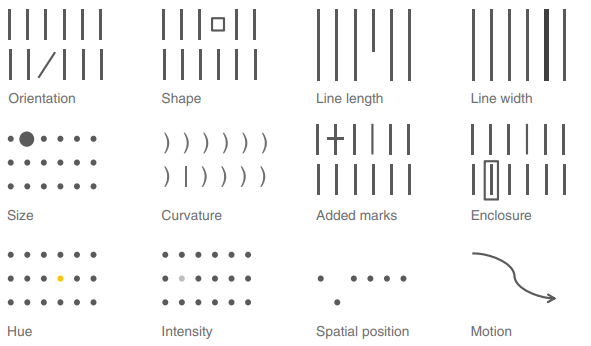
\includegraphics[width=0.8\textwidth]{gfx/preattentive attributes.png}
    \caption{Die präattentiven Attribute von \cite{Knaflic.2016} und \cite{Few.2004}}
    \label{fig:attributes}
    \end{figure}
    Wichtig ist, zu entscheiden, was im Graphen zu den wichtigsten Punkten zählt. Hierzu können etwa folgende Fragen gestellt werden: Welche Aspekte werden sinnvoll hervorgehoben? Was ist eine Ablenkung und kann aus dem Graphen entfernt werden? All diese Punkte sind laut \cite{Knaflic.2016}, \cite{TalksatGoogle.2015} relevant bei dem Bündeln der Aufmerksamkeit des Benutzers.\\
    \item Geschichte erzählen\hfill\\ Im finalen Schritt des Data-Storytellings wird die Geschichte bzw. der Graph logisch aufgebaut. Hierfür müssen ein sinnvoller Anfang und ein Ende festgelegt werden. Zudem soll der Graph ein Fazit und einen Call to Action, also einen Handlungsaufruf, enthalten.
\end{enumerate}
\section{Expertenumfrage mit Auswertung}
Für die fahrzeugspezifischen Daten in der Anwendung sollen in diesem Anwendungsfall auch Trends erkannt werden können, die später mit dem Data-Storytelling angezeigt werden sollen. Da die Trends in den Daten aber spezifisch sind, wurden für das Finden der relevanten Themen in den Daten Experteninterviews durchgeführt. Dabei ist ein Ziel der Befragung, die genauen Punkte, die in den Zeitreihen durch das Data-Storytelling für die Ingenieure hervorgehoben werden sollen, zu definieren und einzugrenzen. Es können insgesamt drei verschiedene Ziele der Umfrage definiert werden:
\begin{enumerate}
    \item Informationen für den ersten Punkt des Data-Storytellings, das Verstehen des Kontextes, sammeln.
    \item Herausfinden, was die relevanten Informationen sind, die in den Graphen dargestellt werden sollen.
    \item Im Falle der Zeitreihen definieren, was es für Trends gibt und wann diese auftreten.
\end{enumerate}
Die Interviews zur Erkennung der Trends werden als qualitative Leitfadeninterviews \cite{Engineering.2018} durchgeführt, um den Experten zu ermöglichen weiter in das Thema einzudringen. Die Experten sind in dem Fall vier Ingenieure, die das Verfahren, mit dem die Daten ausgewertet werden, mitentwickelt haben. Der Leitfaden zu den Interviews sowie Transkriptionen aller Interviews sind in \ref{appendix:interview_trends} zu finden. Die Transkriptionen wurden als vereinfachte Transkription angefertigt, da es für diese Arbeit nicht relevant ist, wie die verschiedenen Sprechweisen der Experten sind. Bei den Experten handelt es sich um Benedikt Mundl \ref{appendix:interview_trends_mundl}, Jeele Böggemann \ref{appendix:interview_trends_boeggemann}, Michael Städele \ref{appendix:interview_trends_staedele} und Florian Zenzinger \ref{appendix:interview_trends_zenzinger}, allesamt Ingenieure mit einer fundierten Erfahrung im Bereich Betriebsfestigkeit von mehr als 45 Jahren. Für das einfachere Prüfen der Textstellen sind im Folgenden die Zeilennummern mit den passenden Textstellen im Anhang verlinkt und durch einen Klick auf die erste Zeilennummer aufrufbar.\\
%line space in nächster Zeile damit die quelle nicht über den fliestext hinausgeht
Um die Interviews wissenschaftlich zu analysieren, wurde MAXQDA\\ \cite{MAXQDA.2023} verwendet und nach den Methoden von \cite{Mayring.2022}, \cite{Kuckartz.2022} und \cite{AndreMorgensternEinenkel.2023} die inhaltlich strukturierende qualitative Inhaltsanalyse erstellt. \\\\Anhand dieser Analyse konnten mehrere Kategorien festgelegt werden, die für das Erkennen der Trends in den Daten von Bedeutung sind. Insbesondere die Kategorien in der Überkategorie Trends sind von Wichtigkeit, da in dieser Kategorie genau die Aussagen zu den Trends erkennbar sind. In der Unterkategorie Aufstiege steigen die Daten über einen Zeitraum an, wie von Michael Städele in den Zeilen \lref{appendix:interview_trends_staedele:aufstiege_1}--390 und \lref{appendix:interview_trends_staedele:aufstiege_2}--449 sowie Benedikt Mundl in den Zeilen \lref{appendix:interview_trends_mundl:aufstiege_1}--116 erläutert wird. Die Kategorie Abstiege ist laut den Interviews weniger relevant, diese wurden nur von Michael Städele in den Zeilen \lref{appendix:interview_trends_staedele:abstiege_1}--390 angesprochen. Die Tatsache, dass die Abstiege nur von einem Experten erwähnt werden, wird später in den Darstellungen von Bedeutung. Bei den Abstiegen handelt es sich um den Gegenpart der Aufstiege, weil die Daten sich hier graduell nach unten entwickeln. Das nächste relevante Element in den Daten sind sogenannte Peaks. Peaks können als Minima oder Maxima in den Daten in Relation zu den umliegenden Werten definiert werden. Laut den Experten Florian Zenzinger (Zeilen \lref{appendix:interview_trends_zenzinger:peaks_1}--599), Michael Städele (Zeilen \lref{appendix:interview_trends_staedele:peaks_1}--449 und Zeilen \lref{appendix:interview_trends_staedele:peaks_2}-473) und Benedikt Mundl (Zeilen \lref{appendix:interview_trends_mundl:peaks_1}--41) werden diese bei der Analyse der Daten als Erstes betrachtet. Rückschließend lässt sich davon ausgehen, dass die Peaks in der Darstellung relevanter sind als beispielsweise die Abstiege. Die nächste Kategorie ist das Offset, auch Drift genannt, hierbei handelt es sich um eine Nullpunktverschiebung in den Daten. Durch das Offset kann beispielsweise eine plastische Verformung am Fahrzeugteil erkannt werden, wie Florian Zenzinger (Zeilen \lref{appendix:interview_trends_zenzinger:offset_1}--730 und \lref{appendix:interview_trends_zenzinger:offset_2}--741), Jeele Böggemann (Zeilen \lref{appendix:interview_trends_boeggemann:offset_1}--352) und Benedikt Mundl (Zeilen  \lref{appendix:interview_trends_mundl:offset_1}--46)  beschreiben. Ein weiteres Datenmuster von Interesse sind Schwingungen, bei denen die Daten zwischen maximalen und minimalen Werten rapide hin und her schwanken. Florian Zenzinger erwähnt Schwingungen in den Zeilen \lref{appendix:interview_trends_zenzinger:schwingungen_1}--678, \lref{appendix:interview_trends_zenzinger:schwingungen_2}--682, \lref{appendix:interview_trends_zenzinger:schwingungen_3}--696, \lref{appendix:interview_trends_zenzinger:schwingungen_4} und \lref{appendix:interview_trends_zenzinger:schwingungen_5}--708, während Michael Städele die Schwingungen in den Zeilen \lref{appendix:interview_trends_staedele:schwingungen_1}--452 beschrieben hat. Ansonsten wurden noch allgemeine Abweichungen beschrieben. Damit sind hauptsächlich Über- oder Unterschreitungen eines bestimmten Wertebereichs gemeint. Diese Abweichungen wurden von Florian Zenzinger in den Zeilen \lref{appendix:interview_trends_zenzinger:abweichungen_1}--607, von Jeele Böggemann in den Zeilen \lref{appendix:interview_trends_boeggemann:abweichungen_1}--246 und \lref{appendix:interview_trends_boeggemann:abweichungen_5}--344 sowie von Benedikt Mundl in den Zeilen \lref{appendix:interview_trends_mundl:abweichungen_1}--134 beschrieben. In Abbildung \ref{fig:trends} werden alle Subkategorien der Trends in visueller Form dargestellt, geordnet nach der Häufigkeit der Erwähnung. 
\begin{figure}[h!]
\centering
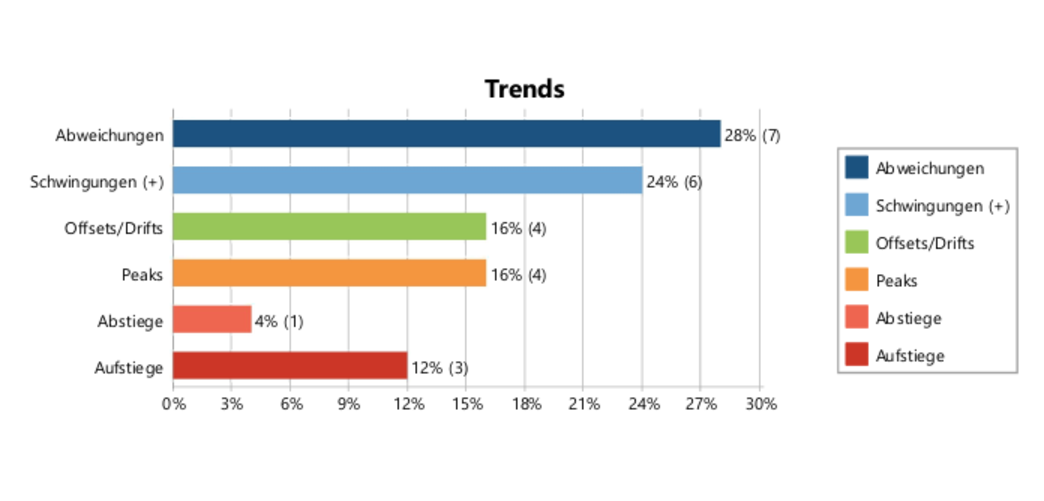
\includegraphics[scale=0.7]{appendix/InterviewTrends/anzahl trends.pdf}
\caption{Die Trendkategorien sortiert nach Häufigkeit der Erwähnung}
\label{fig:trends}
\end{figure}
\\In Bezug auf die Interviews lassen sich auch einige Aussagen zu den Daten allgemein treffen. So wird von Florian Zenzinger in den Zeilen \lref{appendix:interview_trends_zenzinger:daten_1}--717 die Darstellungsmethode \ac{PSD} erklärt. Diese Darstellungsmethode kann laut Herrn Zenzinger bei den Zeitreihen benutzt werden, um die Schwingungen eines Teils darzustellen. Michael Städele (Zeilen \lref{appendix:interview_trends_staedele:daten_1}--431) und Jeele Böggemann (Zeilen \lref{appendix:interview_trends_boeggemann:daten_1}--229, \lref{appendix:interview_trends_boeggemann:daten_2}--270 und \lref{appendix:interview_trends_boeggemann:daten_3}--280) gehen genauer auf die Daten ein, die von den Sensoren geschickt werden. Dabei wird von Michael Städele auch das \ac{DT} erwähnt. Hierbei handelt es sich um das Verfahren, mit dem rechnerisch die Beschleunigungen und Belastungen der Komponenten abgeleitet werden können. Jeele Böggemann erklärt, dass für das Messen \ac{DMS} verwendet werden. In \cite{Keil.2017} wird das Messen mit \ac{DMS} als \glqq [Erfassung der] Dehnungsmessstreifen [von] Dehnungen, die die vom Aufnehmer zu messenden mechanischen Größen im Messkörper des Aufnehmers [hervorrufen]\grqq{}, erklärt. Jeele Böggemann spricht zudem noch von sogenannten Targets, die von Herrn Böggemann als \glqq Wert, mit dem das Fahrzeug abgeprüft wurde\grqq{}, beschrieben werden. In \ref{appendix:general_types} in den Zeilen 51-–73 ist der zum Target passende Datentyp dargestellt.\\\\Zusätzlich zu den allgemeinen Daten werden von den Interviewten auch Aussagen über die Extremwerte und die Schädigungswerte getroffen. Die Extremwerte werden von Florian Zenzinger (Zeilen \lref{appendix:interview_trends_zenzinger:extremwerte_1}--670), von Jeele Böggemann (Zeilen \lref{appendix:interview_trends_boeggemann:extremwerte_1}--235 und \lref{appendix:interview_trends_boeggemann:extremwerte_2}--466) und von Benedikt Mundl (Zeilen \lref{appendix:interview_trends_mundl:extremwerte_1}--27 und \lref{appendix:interview_trends_mundl:extremwerte_2}--176) erwähnt. Sie sind sich einig darüber, dass es sich bei den Extremwerten um die ersten Points of Interest handelt, die sie bei der Analyse prüfen. Daraus resultierend sollen bei der späteren Darstellung von Daten mit dem Data-Storytelling die Extremwerte hervorgehoben werden. Besonders auf \glqq Ausreißer\grqq{} wird bei der Analyse Wert gelegt. Ebenso werden die Schädigungswerte von allen interviewten Personen als wichtig erachtet, von Florian Zenzinger in den Zeilen \lref{appendix:interview_trends_zenzinger:schädigungswerte_1}--677, Michael Städele in den Zeilen \lref{appendix:interview_trends_staedele:schädigungswerte_1}--389 und \lref{appendix:interview_trends_staedele:schädigungswerte_2}--466, Jeele Böggemann in den Zeilen \lref{appendix:interview_trends_boeggemann:schädigungswerte_1}--240 und Benedikt Mundl in den Zeilen \lref{appendix:interview_trends_mundl:schädigungswerte_1}--108, \lref{appendix:interview_trends_mundl:schädigungswerte_2}--110 und \lref{appendix:interview_trends_mundl:schädigungswerte_3}--180. Die Schädigung kann mittels eines Wertes definiert werden, der angibt, wie lange die Lebensdauer eines Bauteils ist.\\
Die Kategorie der Visualisierungen wird in zwei Unterkategorien eingeteilt, die Zeitreihen und die Zählmethoden. Zu den Zählmethoden zählen auch die Erwähnungen von \glqq Kollektiven\grqq{}, vollständig Lastkollektive genannt. Kollektive werden in \cite{Jacobs.2016} definiert als \glqq ein Datensatz, der die Beanspruchung eines Bauteils oder einer Maschine in einem bestimmten Zeitraum abbildet. In einem Lastkollektiv wird der Verlauf der einwirkenden Kraft oder der auftretenden Spannung über [die] Zeit bestimmt\grqq{}. Florian Zenzinger achtet, laut den Zeilen \lref{appendix:interview_trends_zenzinger:zeitreihen_1}--679 und \lref{appendix:interview_trends_zenzinger:zeitreihen_2}--696, in den Zeitreihen besonders auf starke Schwingungen. Indessen wünscht sich Benedikt Mundl laut den Zeilen \lref{appendix:interview_trends_mundl:zeitreihen_1}--190 eine Möglichkeit, mehrere Zeitschriebe miteinander zu vergleichen. Die Zählmethoden werden von Herrn Mundl in den Zeilen \lref{appendix:interview_trends_mundl:zaehlmethoden_1}--186 erwähnt und genauer als Kollektive, Rangepair und Levelcrossing definiert. Laut Jeele Böggemann (Zeilen \lref{appendix:interview_trends_boeggemann:zaehlmethoden_1}--307) ist die Darstellung der Kollektive für ihn besonders relevant. \\\\ Des Weiteren gibt es die Hauptkategorie Plausibilisierung, bei der anhand von automatischer Erkennung direkt überprüft werden sollte, ob die Daten  realistisch und plausibel sind. Die Plausibilisierung allgemein wird von Florian Zenzinger (Zeilen \lref{appendix:interview_trends_zenzinger:plausibilisierung_1}--598) und von Benedikt Mundl (Zeilen \lref{appendix:interview_trends_mundl:plausibilisierung_1}--31) erwähnt. Im Allgemeinen ist bei der Plausibilisierung nur schwierig automatisch zu bestimmen, wann ein Wert realistisch ist, da sich die Ingenieure dabei stark auf ihre Erfahrung verlassen. Aber wenn beispielsweise ein Signal über längere Zeit null ist, obwohl sich das Fahrzeug  bewegt, ist die Wahrscheinlichkeit hoch, dass es sich um einen Defekt oder Messfehler handelt. Hieraus resultiert eine weitere Unterkategorie in der Plausibilisierung: Defekte und Messfehler. Florian Zenzinger (Zeilen \lref{appendix:interview_trends_zenzinger:defekte_1}--616), Michael Städele (Zeilen \lref{appendix:interview_trends_staedele:defekte_1}--445), Jeele Böggemann (Zeilen \lref{appendix:interview_trends_boeggemann:defekte_1}--237) und Benedikt Mundl (Zeilen \lref{appendix:interview_trends_mundl:defekte_1}, \lref{appendix:interview_trends_mundl:defekte_2}--28, \lref{appendix:interview_trends_mundl:defekte_3}--116 und \lref{appendix:interview_trends_mundl:defekte_4}--125) erwähnen allesamt Messfehler oder Defekte an den Sensoren. Solche Fehler erkennt man laut den Interviewten häufig an Peaks, Ausreißern oder an Nullwerten, die von den Sensoren gesendet werden. Auch deswegen sind die Peaks in der Trenderkennung  relevant. Auch bei individuellen Fehlern des Fahrers kann es zu Problemen bei der Plausibilisierung kommen. Jeele Böggemann (Zeilen \lref{appendix:interview_trends_boeggemann:fahrer_1}--274) und Benedikt Mundl (Zeilen \lref{appendix:interview_trends_mundl:fahrer_1}--98 und \lref{appendix:interview_trends_mundl:fahrer_2}--125) sprechen dieses Thema an. Eine Voraussetzung der Messungen ist im Speziellen bei der Dauerlauferprobung ist, die Strecken immer gleich abzufahren. Denn wenn ein Fahrer beispielsweise den Bordstein anfährt oder von der Strecke abkommt, können die Messungen abweichen. Auch hier ist es schwierig, automatisch zu erkennen, wann so ein Fehler vorliegt, da auch das auf der Erfahrung der auswertenden Ingenieure basiert. \\ Zuletzt wurden die interviewten Ingenieure nach den bereits geplanten Unterseiten für die Webseite befragt. Das Dashboard soll laut Florian Zenzinger (Zeilen \lref{appendix:interview_trends_zenzinger:dashboard_1}--659) und Benedikt Mundl (Zeilen \lref{appendix:interview_trends_mundl:dashboard_1}--72) zunächst als Einstieg in die Datenbasis gesehen werden, mit einer Übersicht dazu, welche Einsatzorte und Strecken es in den vorhandenen Daten gibt und welche Fahrzeuge diese abgefahren sind. Zu der Unterseite mit den Vergleichen der Erprobungen und den realen Einsätzen wird von Michael Städele (Zeilen \lref{appendix:interview_trends_staedele:vergleich_1}--551) und Benedikt Mundl (Zeilen \lref{appendix:interview_trends_mundl:vergleich_1}--158 und \lref{appendix:interview_trends_mundl:vergleich_2}-167) angemerkt, dass es sich hier um die wichtigste Unterseite handelt. Der Grund liegt darin, dass durch die Vergleiche berechnet wird, wie ein Fahrzeug voraussichtlich in einem, in der Zukunft liegenden, Einsatz beschädigt wird. Auf der Unterseite der Dauerlauferprobung werden die Daten der Fahrzeuge auf festgelegten Strecken von denselben Fahrern über lange Zeit erprobt. Gleichzeitig werden die Vergleichsdaten gesammelt, die dann auf der Vergleichsseite verwendet werden. Dies wird von Florian Zenzinger (Zeilen \lref{appendix:interview_trends_zenzinger:dauerlauferprobung_1}--646), Michael Städele (Zeilen \lref{appendix:interview_trends_staedele:dauerlauferprobung_1}--511 und \lref{appendix:interview_trends_staedele:dauerlauferprobung_2}--539), Jeele Böggemann (Zeilen \lref{appendix:interview_trends_boeggemann:dauerlauferprobung_1}--299) sowie Benedikt Mundl (Zeilen \lref{appendix:interview_trends_mundl:dauerlauferprobung_1}--80, \lref{appendix:interview_trends_mundl:dauerlauferprobung_2}--105, \lref{appendix:interview_trends_mundl:dauerlauferprobung_3}--108 und \lref{appendix:interview_trends_mundl:dauerlauferprobung_4}--144) übereinstimmend bestätigt. \\\\ Zum Data-Storytelling haben Michael Städele (Zeilen \lref{appendix:interview_trends_staedele:storytelling_1}--402, \lref{appendix:interview_trends_staedele:storytelling_2}--412 und \lref{appendix:interview_trends_staedele:storytelling_3}--557) und Florian Zenzinger (Zeilen \lref{appendix:interview_trends_zenzinger:storytelling_1}--664) einige Ideen für potenzielle Datengeschichten, unter anderem, wo ein Einsatz extrem ist, wie die Bodenbeschaffenheit ist oder wie sich eine Erprobung im Vergleich zu einem tatsächlichen Einsatz verhält. Allgemein zur Entwicklung werden von Jeele Böggemann (Zeilen \lref{appendix:interview_trends_boeggemann:wunsch_1}--316, \lref{appendix:interview_trends_boeggemann:wunsch_2}--329 und \lref{appendix:interview_trends_boeggemann:wunsch_3}--339) und Benedikt Mundl (Zeilen \lref{appendix:interview_trends_mundl:wunsch_1}--199) einige kleinere Wünsche geäußert, eine Funktion zum Sortieren von Balkendiagrammen, vermehrter Einsatz von Hovereffekten zur besseren Einordnung von speziellen Punkten und der Vergleich von Zeitschrieben. Zur besseren Übersicht werden die Ergebnisse der Experteninterviews in Tabelle \ref{2:experteninterview_results} mit einer kurzen Beschreibung und der Häufigkeit der Erwähnungen dargestellt.
\newpage
\label{2:experteninterview_results}
\begin{table}[h!]
\begin{tabular}{p{4cm}|p{6.7cm}|r}
Liste der Kategorien                & Beschreibung                                                                                   & Häufigkeit \\ \hline \hline
Trends                               &                                                                                                &                                \\
\hspace{5mm}Aufstiege                            & Eine graduelle Veränderung der Daten nach oben                                                 & 3                              \\
\hspace{5mm}Abstiege                             & Eine graduelle Veränderung der Daten nach unten                                                & 1                              \\
\hspace{5mm}Extremwerte                                & Ein signifikanter Spitzenwert in den Daten, negativ oder positiv                                                     & 4                              \\
\hspace{5mm}Offset/Drifts                        & Eine Nullpunktverschiebung in den Daten                                                        & 4                              \\
\hspace{5mm}Schwingungen                         & Wiederholte Schwankungen in den Daten                                                          & 6                              \\
\hspace{5mm}Abweichungen                         & Überschreitung der Daten aus dem zuvor festgelegten Wertebereich                                    & 4                            \\ \hline  
Daten                                & Allgemeine Aussagen zu den benutzten Daten                                                      & 5                              \\
\hspace{5mm}Extremwerte                          & Extreme Punkte in den Daten                                                               & 5                              \\
\hspace{5mm}Schädigungswerte                     & Die allgemeine Bezeichnung der Daten, die für die Schädigung einer Komponente berechnet werden  & 7                              \\ \hline  
Visualisierungen                     &                                                                                                &                                \\
\hspace{5mm}Zeitreihen                           & Daten über einen Zeitraum dargestellt                                                   & 3                              \\
\hspace{5mm}Zählmethoden     & In der Mechanik bereits existierende Arten von Darstellungen                                   & 2                              \\  \hline  
Plausibilisierung                    &                                                                                                &                                \\
\hspace{5mm}Defekte/Messfehler               & Defekte oder Messfehler der Sensoren in den Daten                                              & 7                              \\
\hspace{5mm}Fehler des Fahrers                   & Erkennung von individuellen Fehlern beim Fahren, Missuse oder sonstigen Inkonsistenzen                       & 3                              \\    \hline  
Dashboard                            & Aussagen zu der Unterseite Dashboard                                                           & 2                              \\   \hline  
Überwachung Dauerlauferprobung       & Aussagen zu der Unterseite Überwachung Dauerlauferprobung                                      & 8                              \\   \hline  
Vergleiche von Einsatzdaten          & Aussagen zu der Unterseite Vergleiche von Einsatzdaten                                         & 3                              \\\hline  
Data-Storytelling                    & Allgemeine Ideen zum Thema Data-Storytelling und im speziellen Vorschläge für Datengeschichten & 4                              \\\hline  
Wünsche                              & Allgemeine Wünsche für die Darstellungen                                                       & 4                            
\end{tabular}
\centering
\caption {Ergebnisse der Experteninterviews mit Kurzbeschreibungen und Häufigkeiten der Erwähnungen des Themas}
\end{table}

\newpage

\section{Regeln zum Erkennen von Trends in den Zeitreihendaten}
Um die Erkennung der Trends in den Zeitreihen dynamisch ausführen zu können, müssen für jede Art der Erkennung Regeln festgelegt werden, die dann durch die Implementierung die Trends erkennen. Die Implementierung ist in \ref{appendix:trend-detection-code} zu finden und in TypeScript implementiert, um für den Benutzer dynamisch anpassbar zu sein. Thematisch wird die Trenderkennung für Zeitreihen (siehe Datentyp \texttt{TimeSeries} \ref{appendix:graph_types}) implementiert, da diese die Auswirkungen der Kräfte auf verschiedene Komponenten über die Dauer der Messung anzeigen. Die Zeitreihen setzen sich aus dem Nummern-Array \texttt{values} und einer Frequenz, in der die Werte auftreten, zusammen. Die Frequenz wird mit der Anzahl der Werte verrechnet, um die x-Werte zu erzeugen. Die y-Werte bildet der \texttt{values}-Array. Dadurch, dass die Werte der Zeitreihen immer in der gleichen Frequenz auftreten, ist gegeben, dass die einzelnen Datenpunkte stets die gleiche Distanz zueinander haben.
\subsection{Allgemeine Regeln und Funktionen}\label{2:general_implementations}
Für die Berechnungen werden viele Funktionen mehrfach benötigt. Um Code-Wiederholungen zu vermeiden, bessere Lesbarkeit zu ermöglichen und das Testen der Funktionen zu erleichtern, werden hilfreiche Mikrofunktionen erstellt, die in mehreren der Trenderkennungsfunktionen benötigt und genutzt werden. Im Folgenden werden diese kurz erklärt und zusammenfassend dargestellt:
\begin{description}

\item[\texttt{average}] \hfill \\\\
Die Berechnung des arithmetischen Mittels, dargestellt in \ref{appendix:trend-detection-code}[Zeilen 7-–9]. Eine einfache Funktion, die die Datenpunkte annimmt, diese so anpasst, dass alle Werte miteinander addiert werden, und zum Schluss die Summe durch die Anzahl der Werte in dem entsprechenden Array teilt. Die Funktion basiert auf der folgenden mathematischen Formel \ref{eqn:average} aus \cite{Papula.2017}:
\begin{equation}
\label{eqn:average}
         average(x_t)=\frac{x_1+x_2+...+x_n}{n}=\frac{\sum\limits_{i=1}^nx_t}{n} 
\end{equation}

\item[\texttt{getPercentageOfHeight}] \hfill \\\\
Diese Funktion (\ref{appendix:trend-detection-code} Zeilen 18-–22) berechnet den maximalen Wertebereich des Arrays und errechnet anhand einer eingegebenen Prozentzahl die prozentuale Höhe. Hierfür wird der in JavaScript, und somit auch TypeScript, vorhandene Built-in Namespace \texttt{Math} \cite{MDNcontributors.} verwendet, um die maximalen und minimalen Werte des Arrays auszugeben. Dadurch ist die Funktion einfach zu testen und performant. In der folgenden Formel \ref{eqn:height} wird der Rechenweg wiedergegeben, wobei es sich bei der Variable \texttt{p} um die eingegebene Prozentzahl handelt.\\ 
\begin{equation}
\begin{split}
\label{eqn:height}
 height(x_t,p)&=(\max(x_1, x_2, ..., x_n) - \min(x_1, x_2, ..., x_n)) * p \\
&\text{für } \{p \in \mathbb{Q}| 0.01 < p \le 1.00 \}
\end{split}
\end{equation}


\item[\texttt{getPercentageOfDistanceBetweenMarkers}] \hfill \\\\
Ähnlich wie auch bei \texttt{getPercentageOfHeight} wird mit dieser Funktion (\ref{appendix:trend-detection-code} Zeilen 31-–36) berechnet, wie viele Marker wie viel Prozent der gesamten Länge der Zeitreihe entsprechen. Da alle Datenpunkte gleich weit voneinander entfernt sind, lässt sich anhand des Ergebnisses später einfach durch Einsetzen in die Frequenzberechnung erkennen, wo sich die Marker befinden. Daraus bildet sich die mathematische Formel \ref{eqn:distance}.\\
\begin{equation}
\begin{split}
\label{eqn:distance}
    distance(p,n)&= p * n\\ 
    &\text{ wobei }n\text{ der Länge der Zeitreihe entspricht}\\ &\text{ und für }p\text{ gilt }\{p \in \mathbb{Q}| 0.01 < p \le 1.00 \}.\\\
\end{split}
\end{equation}

\item[\texttt{getMovingAverage}]\hfill \\\\
Bei der Funktion \texttt{getMovingAverage} (\ref{appendix:trend-detection-code}, 44-–73) handelt es sich um eine Funktion, die den gleitenden Durchschnitt der Zeitreihe berechnet und diesen als Gleitkommazahlen-Array zurückgibt. Die Funktion ist inspiriert durch das \texttt{optimal solution example} von \cite{RichardBevan.}, wobei die Funktion anhand der mathematischen Formel in \ref{eqn:moving-average} so weit angepasst wurde, dass nur noch die Zeile 56 von der Funktion von \cite{RichardBevan.} vorhanden ist. Der gleitende Durchschnitt ist für die Trenderkennung ein wichtiges Werkzeug \cite{Wiesbaden.2013} und wird von \cite{Hyndman.2011} definiert als Zeitreihe, die aus mehreren Durchschnitten von mehreren aufeinanderfolgenden Werten einer anderen Zeitreihe gebildet wird. Für die Berechnung wird ein \texttt{window} festgelegt, das die Anzahl der Werte festlegt, die für die Durchschnittsberechnung einbezogen werden sollen. Das bedeutet allerdings auch, dass somit die Durchschnittswerte für den Anfang und das Ende der Zeitreihe nicht berechnet werden können. Aus diesen Gründen wurden die Zeilen 48–-56 und 65-–71 ergänzt. Dabei wird für den Anfangs- und Endbereich jeweils eine gleitende Durchschnittsberechnung ausgeführt, die nur in die jeweilige Richtung, die vorhanden ist, berechnet, anstatt das \texttt{window} in beide Richtungen vom Ausgangswert zu verschieben. Dadurch wird das Ergebnis-Array gefüllt, damit später die Anzahlen des Ergebnisarrays und des Arrays der tatsächlichen Zeitreihe miteinander übereinstimmen. Das ist wichtig, da auch die Frequenz, in der die Werte auftreten, übereinstimmen muss, damit beispielsweise beim Bilden der Auf- und Abstiege die richtigen Positionen angegeben werden.  Da sich das \texttt{window} dynamisch aus der Anzahl der Punkte der tatsächlichen Zeitreihe und einem festen Wert bildet, wurde die Zeile 45 ergänzt, um Rechenfehler zu vermeiden. Mit der Standardfunktion \texttt{toFixed()} wird eine Zahl in einen String umgewandelt und dabei wird die Länge der Dezimalstellen auf null begrenzt. Das + vor \texttt{window.toFixed()} wandelt den String automatisch wieder in eine Zahl um. In Abbildung \ref{fig:movingAverage} wird eine Zeitreihe mit dem gleitenden Durchschnitt berechnet, durch die Funktion mit einem \texttt{window} von der Länge des Arrays geteilt, durch den Faktor 50 dargestellt. Da die Zeitreihen variable Längen haben, soll, weil das \texttt{window} dadurch von der Länge der Zeitreihe abhängt, gewährleistet werden, dass der gleitende Durchschnitt sich verhältnismäßig bei allen Zeitreihen gleich verhält. 

\begin{figure}[h!]
\centering
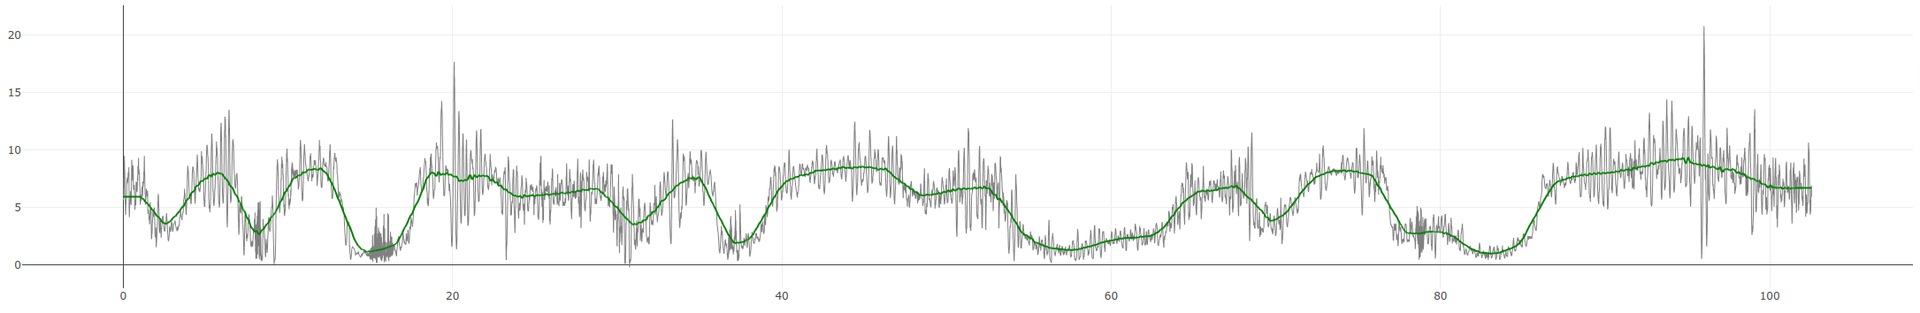
\includegraphics[width=\textwidth]{gfx/movingAverage.png}
\caption{Gleitender Durchschnitt}
\label{fig:movingAverage}
\end{figure}
Mathematisch wird der gleitende Durchschnitt ungerader Ordnung von \cite{Bosch.2002} definiert als:
\begin{equation}
\label{eqn:moving-average}
    \begin{split}
        movingAverage(x_t,m)&=\frac{1}{2m+1}(x_{t-m}+x_{t-m+1}+...+x_t+...+x_{t+m})\\
&=\frac{1}{2m+1}\sum\limits_{j=-m}^mx_{t+j} \text{ mit }\{m\in \mathbb{N}\}\\
    \end{split}
\end{equation}
Dabei steht $m$ für das \texttt{window}, das für den gleitenden Durchschnitt festgelegt wurde, und $x_t$ für die Zeitreihe.
Da bei der Erstellung des gleitenden Durchschnitts ungerader Ordnung jeweils am Anfang und am Ende der Zeitreihe \[k=\frac{m}{2}\] herausfallen, werden diese Werte bei der Implementation am Anfang der Zeitreihe mit \[\frac{1}{m+1}(x_{t}+x_{t+1}+...+x_{t+m})\] und am Ende der Zeitreihe mit  \[\frac{1}{m+1}(x_{t-m}+x_{t-m+1}+...+x_t)\] ergänzt. \\\\

\item[\texttt{findLocalExtreme}]\hfill \\\\
Die Funktion (\ref{appendix:trend-detection-code} Zeilen 81-–99) findet lokale Minima und lokale Maxima der Zeitreihe und gibt diese aus. Die Funktion basiert auf der Implementation von \cite{SamuelProll.2022} und wurde hier so weit abgeändert, dass damit nicht nur Maxima, sondern auch Minima gefunden werden können (Zeilen 86, 91–-97). Es wurde eine boolesche Variable \texttt{findMaxima} hinzugefügt, die zwischen der Suche nach Minima und Maxima unterscheidet. Die Funktion iteriert durch alle Punkte des Wert-Arrays und vergleicht die direkten Nachbarn mit dem aktuellen Punkt. Bei den Maxima müssen der linke und rechte Nachbar jeweils niedriger sein als der aktuelle Punkt. Bei den Minima ist diese Bedingung genau umgekehrt, beide Nachbarn müssen also höher sein als der aktuelle Punkt. In der folgenden Formel \ref{eqn:minmax} werden die Bedingungen mathematisch formuliert.
\begin{equation}
\label{eqn:minmax}
    \begin{split}
        &\text{Im Folgenden steht }x_t\text{ für die Zeitreihe und }n\text{ für die Länge dieser.}\\
       & \text{Wenn Maxima gesucht werden:}\\&
        	Maxima(x_t, n)=\{ x_i \in {1, 2, ..., n}| x_i > x_{i-1} \wedge x_i > x_{i+1}\}\\
         & \text{Wenn Minima gesucht werden:}\\&
        	Minima(x_t, n)=\{ x_i \in {1, 2, ..., n}| x_i < x_{i-1} \wedge x_i < x_{i+1}\}\\
    \end{split}
\end{equation}
\end{description}

\subsection{Aufstiege und Abstiege}
\label{subsection:risesAndFalls}
Die Berechnungen für die Auf- und Abstiege funktionieren ähnlich zueinander. Der entsprechende Code ist in \ref{appendix:trend-detection-code:aufstiege} zu sehen. Zur Vermeidung von Wiederholungen wird nur die Funktion für die Aufstiege erklärt, da die Funktion für die Abstiege sich allein durch die Bedingungen in den If-Abfragen unterscheidet. Für die Funktion werden ausschließlich die y-Werte benötigt. Die Funktion kann aber, falls gewünscht (für das Data-Storytelling), mit Benutzereingaben erweitert werden. Aus Performancegründen wird ebenso der gleitende Durchschnitt als Variable in die Funktion mit übergeben, da der gleitende Durchschnitt von mehreren Funktionen der Trenderkennung genutzt wird und so nur einmal berechnet werden muss. Die Funktion liefert einen Array aus Anfangs- und Endpunkten der Anstiege. Wichtig für die Erkennung der Aufstiege sind folgende Variablen, die auch durch den Nutzer manuell eingegeben werden können:
\begin{itemize}
    \item Minimale Distanz zwischen dem Start- und Endpunkt in Prozent, um die minimale Länge eines Anstiegs/Abstiegs festzulegen
    \item Minimale Höhe zwischen den Start- und Endwerten in Prozent
\end{itemize}
Grundlegend funktioniert die Berechnung so: Der gleitende Durchschnitt wird Punkt für Punkt durchgegangen und jeder Punkt wird mit seinen Nachbarn verglichen. Befindet sich der Punkt in einem Anstieg, ist sein linker Nachbar niedriger und sein rechter Nachbar höher, wird der Punkt übersprungen. Ist der Punkt der Anfang eines Anstiegs, also der linke Nachbar höher oder gleich hoch und der rechte Nachbar ebenso höher ist, wird der Punkt als Startpunkt angesehen. Es kann nur ein Endpunkt erkannt werden, wenn bereits ein definierter Startpunkt gefunden wurde und wenn der aktuelle Punkt höher als der linke Nachbar ist und niedriger oder gleich hoch wie der rechte. Wenn ein definierter Startpunkt und ein definierter Endpunkt existieren, diese Punkte auch im Array der \texttt{values} vorhanden sind, also bei der Erstellung des gleitenden Durchschnitts keine Fehler aufgetreten sind, dann kann geprüft werden, ob der Anstieg durch die minimale Distanz und die minimale Höhe auch als Anstieg zugelassen werden soll. Nachdem geprüft worden ist, ob ein Start- und Endpunkt als Anstieg zählen, und diese ggf. in das Ergebnisarray \glqq gepusht\grqq{} worden sind, werden der aktuelle Start- und Endpunkt entfernt, damit der nächste Anstieg erkannt werden kann.
Die Abstiegsfunktion unterscheidet sich durch die Bedingungen, unter denen ein Start- oder Endpunkt erkannt wird. Diese sind genau gegensätzlich zu den Anstiegen. In Abbildung \ref{fig:risesAndFalls} werden sowohl die Anstiege als auch die Abstiege und der gleitende Durchschnitt, erkannt durch den beschriebenen Code, dargestellt. Für die Variablen wurde bei An- und Abstiegen als minimale Distanz zwischen den Punkten 1 \% und als minimale Höhe 20 \% angegeben. 
\begin{figure}[h!]
\centering
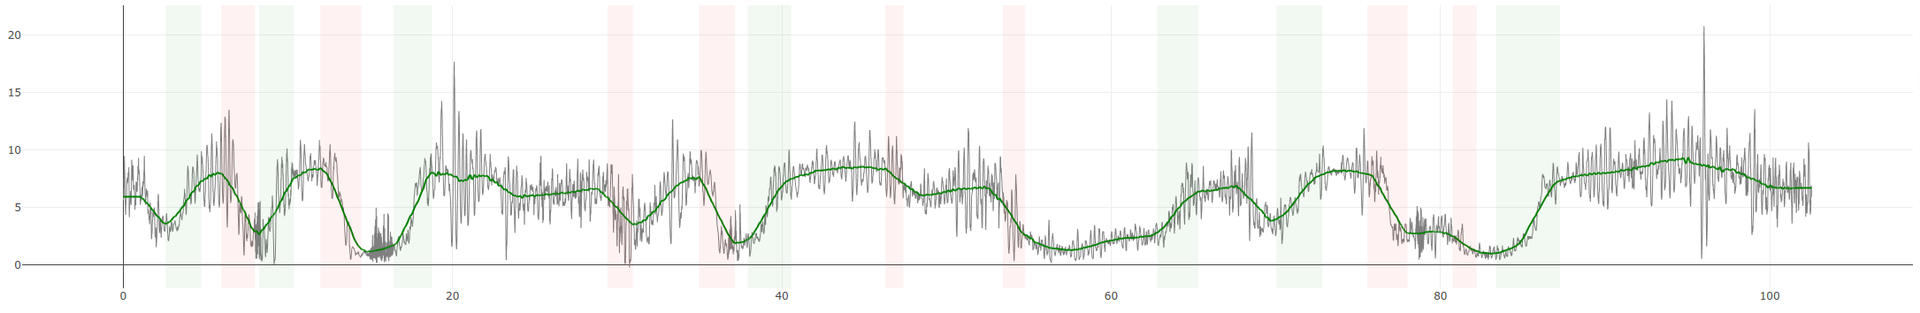
\includegraphics[width=\textwidth]{gfx/falls_rises_movingAverage.png}
\caption{Aufstiege und Abstiege mit gleitendem Durchschnitt}
\label{fig:risesAndFalls}
\end{figure}

\subsection{Extremwerte}
Die Funktion zum Erkennen der Extremwerte (\ref{appendix:trend-detection-code:peaks}) basiert auf \cite{SamuelProll.2022}, der Funktionalitäten von SciPy zum Finden von Peaks in JavaScript konvertiert hat. SciPy ist eine Ansammlung von mathematischen Algorithmen basierend auf NumPy \cite{TheSciPycommunity.2023}, wobei NumPy eine Python Library ist, die auf Simulationswissenschaften spezialisiert ist \cite{NumPyDevelopers.2022}. Ebenso wurde in der Erkennung eine Funktion für einen \texttt{argsort} benötigt, diese basiert auf \cite{EranW.2020}, da es in JavaScript keinen nativen \texttt{argsort} gibt. Ähnlich zu den Aufstiegen und Abstiegen kann auch bei den Extremwerten durch verschiedene Variablen beeinflusst werden, wie präzise die Erkennung ist. Dazu gibt es die folgenden Variablen, alle in Prozent angegeben:
\begin{itemize}
    \item Minimale Höhe von Maxima 
    \item Maximale Höhe von Minima
    \item Distanz zwischen den einzelnen Werten
    \item Puffer zum gleitenden Durchschnitt
\end{itemize}
Die Funktion \texttt{detectExtremesInData} (222--276) startet die Erkennung von Minima und Maxima und berechnet die vom Benutzer eingegebenen Parameter. Dazu werden die Hilfsfunktionen in \ref{2:general_implementations} genutzt. Danach wird die Berechnung an die Funktion \texttt{findExtremes} weitergeleitet. \texttt{findExtremes} ruft zuerst die Funktion \texttt{findLocalExtreme} auf, um die Extremwerte zu bestimmen. Anschließend werden die Werte anhand der oben genannten Variablen gefiltert. Hierbei kann auch komplett auf die Filter verzichtet werden, da diese optional sind. Als Erstes wird nach der Höhe der Werte gefiltert (Zeilen 32–-41). Dazu wird die Built-in-Funktion \texttt{Array.prototype.filter()} verwendet. Es wird unterschieden, ob Minima oder Maxima gefunden werden sollen, und anhand dessen unter oder über der Höhe gefiltert. Um die Funktion auch bei Zeitreihen einzusetzen, die negative Werte erreichen, muss die berechnete Höhe von dem kleinsten Wert der Zeitreihe abgezogen werden. Mathematisch lässt sich diese Funktion folgendermaßen definieren \ref{eqn:filterMinMax}:
\begin{equation}
\label{eqn:filterMinMax}
\begin{split}
   & \text{Filtern der Höhe von Maxima}\\
    &filterByHeight(extremes, x_t, height) = \{x_i \in extremes|x_i>(min(x_t)+height)\}\\
   &\text{Filtern der Höhe von Minima}\\
   & filterByHeight(extremes, x_t, height) = \{x_i \in extremes|x_i<(min(x_t)+height)\}\\
   \\
    \end{split}
\end{equation}
Als Nächstes wird nach Distanz gefiltert, diese Funktion basiert auf \cite{SamuelProll.2022}, wobei die Funktion für das Filtern nach Minima in den Zeilen 59–-62 ergänzt wurde. Bei der Funktionsweise ist wichtig zu erwähnen, dass die Funktion nicht nur nach der Distanz der Werte filtert, sondern dabei auch berücksichtigt, welcher Extremwert höher (oder tiefer) ist, und sich dann je nachdem für den höheren (oder tieferen) Extremwert entscheidet. Die Funktion von \cite{SamuelProll.2022} unterscheidet sich laut dem Autor nur leicht von der SciPy-Implementation und wurde hauptsächlich davon übernommen. Zunächst werden die bereits gefundenen und über die Höhe gefilterten Indices der Extremwerte auf ihre tatsächlichen Höhen gemappt. Danach wird durch die Funktionen von \cite{EranW.2020} der \texttt{argsort} durchgeführt. Laut \cite{NumPyDevelopers.2024} gibt eine \texttt{argsort}-Funktion die Indices aus, wie sie sortiert würden. Um die Funktionen auch für negative Werte in der Zeitreihe zu optimieren, wurde Zeile 23 im Code erweitert. Die native JavaScript-\texttt{sort()}-Funktion sortiert Werte lexikografisch \cite{MDNcontributors.2024}. Das funktioniert in gewisser Weise auch mit Zahlen, da diese einfach zu Strings konvertiert werden. Werden die Zahlen allerdings komplexer oder auch nur negativ, muss in der \texttt{sort()}-Funktion explizit definiert werden, wie sortiert werden soll. Je nachdem, ob Minima oder Maxima gesucht werden, wird danach die Reihenfolge der sortierten Höhen umgedreht. Dann wird im Code in der Reihenfolge der Höhe analysiert, wie weit die Nachbar-Extremwerte vom aktuellen Extremwert entfernt sind, und je nachdem werden die ggf. überflüssigen Extremwerte aus dem Ergebnis entfernt. Dadurch werden automatisch die höchsten Werte behalten, da diese die ersten sind, die verglichen werden.\\\\Zuletzt werden die übrigen Extremwerte über den gleitenden Durchschnitt gefiltert. Diese Funktionalität wurde zu den Funktionen von \cite{SamuelProll.2022} ergänzt. Anhand des eingegebenen Puffers werden nur die Extremwerte übernommen, die einen definierten Abstand vom gleitenden Durchschnitt überschreiten. Hierfür wird der Wert des aktuellen Extremwertes mit dem gleitenden Durchschnitt an der gleichen Stelle verglichen, abzüglich oder zuzüglich (je nachdem, ob Minima oder Maxima gefunden werden sollen) des Puffers. Dabei lautet die mathematische Notation dieser Bedingungen wie in Formel \ref{eqn:filterMovingAverage} dargestellt.
\begin{equation}
\label{eqn:filterMovingAverage}
    \begin{split}
        &\text{Filtern mit dem gleitenden Durchschnitt von Maxima}\\
        &filterMA(extremes,x_t,mA_t, buffer) = \{i \in extremes|x_i>(mA_i+buffer)\}\\
        &\text{Filtern mit dem gleitenden Durchschnitt von Minima}\\
        &filterMA(extremes,x_t,mA_t, buffer) = \{i \in extremes|x_i<(mA_i-buffer)\}
        \\\\
    \end{split}
\end{equation}
In Abbildung \ref{fig:peaks} wird die Extremwerterkennung für Minima und Maxima durchgeführt. Als Variablen wurden für die minimale Höhe der Maxima 75 \%, für die maximale Höhe der Minima 25 \%, als Distanz zwischen den Werten 2 \% und als Puffer 20 \% angegeben. Besonders bei den Minima ist zu sehen, dass die Filterung durch den gleitenden Durchschnitt unbedingt nötig ist, da sich ein Großteil des Signals unter 25 \% Höhe befindet. Für die bessere Erkennbarkeit der Peaks wird in Abbildung \ref{fig:peaks} nur ein Teil der Zeitreihe dargestellt.
\begin{figure}[h!]
\centering
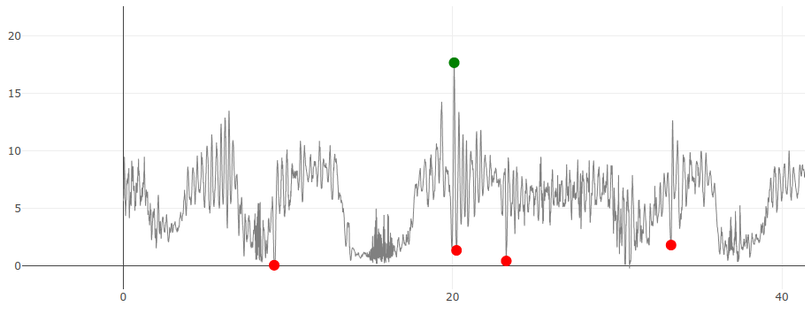
\includegraphics[width=\textwidth]{gfx/peaks.png}
\caption{Maxima und Minima}
\label{fig:peaks}
\end{figure}


\subsection{Offsets und Drifts}
Wie in den Interviews (Kapitel \ref{2:experteninterview_results}) erklärt wird, handelt es sich bei Offsets und Drifts um ein Phänomen, das auftritt, wenn Bauteile plastisch verformt werden. Von den Experten wird bestätigt, dass das Offset und auch Drifts dann erkennbar werden, wenn der Durchschnittswert am Anfang und der Durchschnittswert am Ende eines Graphen drastisch divergieren. Offset und Drift unterscheiden sich durch die Art der Veränderung am Durchschnittswert. Bei Drifts handelt es sich um eine Verschiebung über die Zeit, bei Offsets ist die Verschiebung eher ruckartig. In der Implementation der Funktion zur Erkennung des Offsets in \ref{appendix:trend-detection-code:offsets} lässt sich in den Zeilen 2 und 3 erkennen, dass die gelieferten Daten jeweils in eine vordere Hälfte und eine hintere Hälfte eingeteilt werden und danach die allgemeine Funktion zum Berechnen des Durchschnitts (siehe \texttt{average} \ref{2:general_implementations}) aufgerufen wird. Hierzu wird die \texttt{Array.prototype.slice()}-Funktion von klassischem JavaScript verwendet \cite{MDNcontributors.2020}. In Zeile 6 wird der Pufferwert rechnerisch bestimmt, der gemeinsam mit dem Durchschnittswert des ersten Arrays überschritten  sein muss, um die Offset-Warnung bei kleinen Unterscheidungen zu vermeiden. Schließlich tritt das Offset nur bei drastischen Unterschieden auf. Der Pufferwert wird durch eine Erhöhung von 10\,\% und die allgemeine Funktion von \texttt{getPercentageOfHeight} aus \ref{2:general_implementations} festgelegt. Wenn die Graphen später mit Data-Storytelling überarbeitet werden, lässt sich dieser hart codierte Wert noch durch eine Benutzereingabe ersetzen. Abschließend wird geprüft, ob die Summe des Durchschnitts der ersten Hälfte und des Pufferwerts kleiner ist als die Summe des Durchschnitts der zweiten Hälfte (Zeile 7). Wenn dies zutrifft, wird eine plotly.js-Annotation von der Funktion zurückgegeben, die als Fehlermeldung abgebildet wird.

\subsection{Schwingungen}
Sollten Minima und Maxima direkt aufeinanderfolgen, wird das in dieser Arbeit als Schwingung definiert. Die passende Funktion zu der Schwingungserkennung ist in \ref{appendix:trend-detection-code:schwingungen} nachzuvollziehen. Auch die Schwingungserkennung ist durch Eingaben anpassbar:
\begin{itemize}
    \item Höhe zwischen Minima und Maxima
    \item Distanz zwischen Minima und Maxima
\end{itemize}
Da die Extremwerte bereits mit der \texttt{findLocalExtreme}-Funktion erkannt werden, hat diese Funktion hauptsächlich den Zweck, Minima und Maxima zu vergleichen und zu prüfen, ob sie den eingegebenen Variablen entsprechen. Dazu wird zuerst die Reihenfolge des Auftretens dahingehend geprüft, ob der Maximalwert oder der Minimalwert zuerst eintritt. Aufgrund dieser Prüfung kann je nachdem, welcher Wert zuerst kommt, bestimmt werden, ob die Distanz zwischen den Extremwerten die eingegebene Distanz übersteigt. Wenn dies zutrifft, wird die Höhe der Schwingung geprüft. Wenn beide Bedingungen, also die Höhe der Schwingung und die Distanz zwischen den Extremwerten, erfüllt sind, wird die Kombination aus Maxima und Minima als Schwingung zurückgegeben. In Abbildung \ref{fig:vibrations} wurden die Schwingungen mit einer Distanz von 1\,\% und einer Höhe von 30\,\% festgelegt. 
\begin{figure}[h!]
\centering
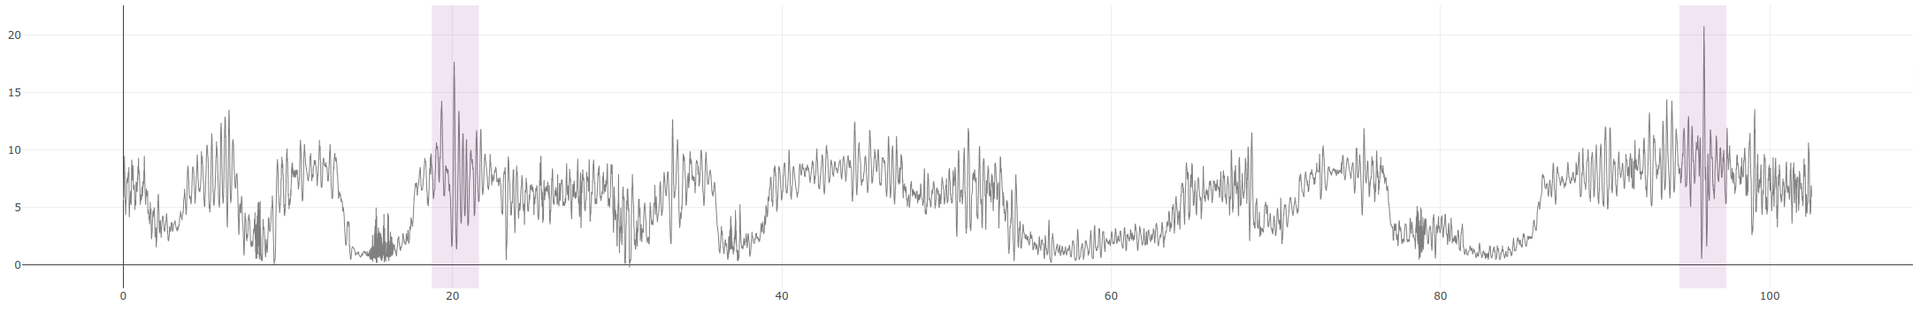
\includegraphics[width=\textwidth]{gfx/vibrations.png}
\caption{Schwingungen}
\label{fig:vibrations}
\end{figure}

\subsection{Abweichungen}
Eine Abweichung wurde von den Experten (siehe Kapitel \ref{2:experteninterview_results}) als Ausbruch aus einem gewissen Wertebereich beschrieben. Hierfür kann der Benutzer entweder einen speziellen Wertebereich für die Markierungen eingeben oder die Funktion in \ref{appendix:trend-detection-code:abweichungen} kann durch die Eingabe eines Puffers einen Wertebereich berechnen, der sich am Durchschnitt aller y-Werte orientiert. Sollte der Benutzer keinen Puffer eingegeben haben, wird mit einem Defaultwert von 20\,\% Puffer gerechnet. Dazu wird mit der allgemeinen \texttt{average}-Funktion der gesamte Durchschnitt ermittelt und dann der Puffer addiert, um die obere Grenze des Wertebereichs, bzw. der Puffer subtrahiert, um die untere Grenze des Wertebereichs zu berechnen. In Abbildung \ref{fig:deviations} werden die Grenzen des Wertebereichs mit 20\,\% Puffer abgebildet. Aus Gründen der besseren Erkennbarkeit wird nur ein Teil der Zeitreihe in \ref{fig:deviations} dargestellt.
\begin{figure}[h!]
\centering
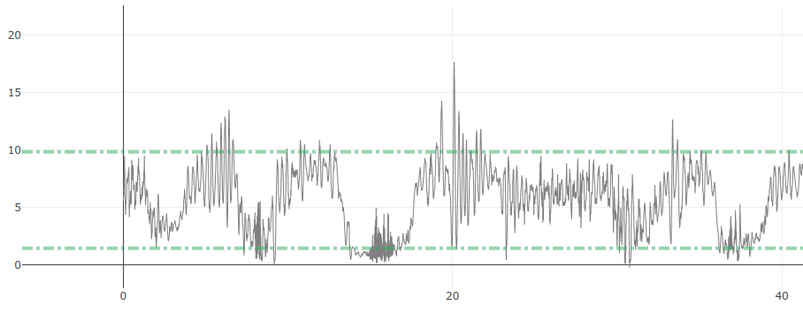
\includegraphics[width=\textwidth]{gfx/deviations.png}
\caption{Abweichungen}
\label{fig:deviations}
\end{figure}
\section{Anwendung des Data-Storytelling}
Im Folgenden werden die Methoden aus \ref{sec:methoden} auf die tatsächlichen Graphen angewandt und implementiert.
\subsection{Prozentuale Schädigung zum groben Überblick}\label{section:Prozentuale_Schädigung}
Grundlegend wird die Datenbasis genutzt, um einen kurzen Überblick über die gesamte Datenlage zu bekommen. Auf der Datenbasis soll ein Graph mit Data-Storytelling entwickelt werden. Wählt man über die Fahrzeugkarten ein einzelnes Fahrzeug aus, soll das kumulierte Lastgeschehen der bewerteten Baugruppen dargestellt werden. \\\\
1. Kontext verstehen:\\
Wie von \cite{Knaflic.2016} empfohlen, wird zunächst Storyboarding mit Stift und Papier betrieben, um einen generellen Entwurf für den Graphen anzufertigen. Danach wird das Tool Figma \cite{FigmaGmbH.2024} genutzt, um einen groben Entwurf zu erstellen. Dieser grobe Entwurf ist in Abbildung \ref{fig:datenbasis} dargestellt.

\begin{figure}[h!]
\centering
\fbox{
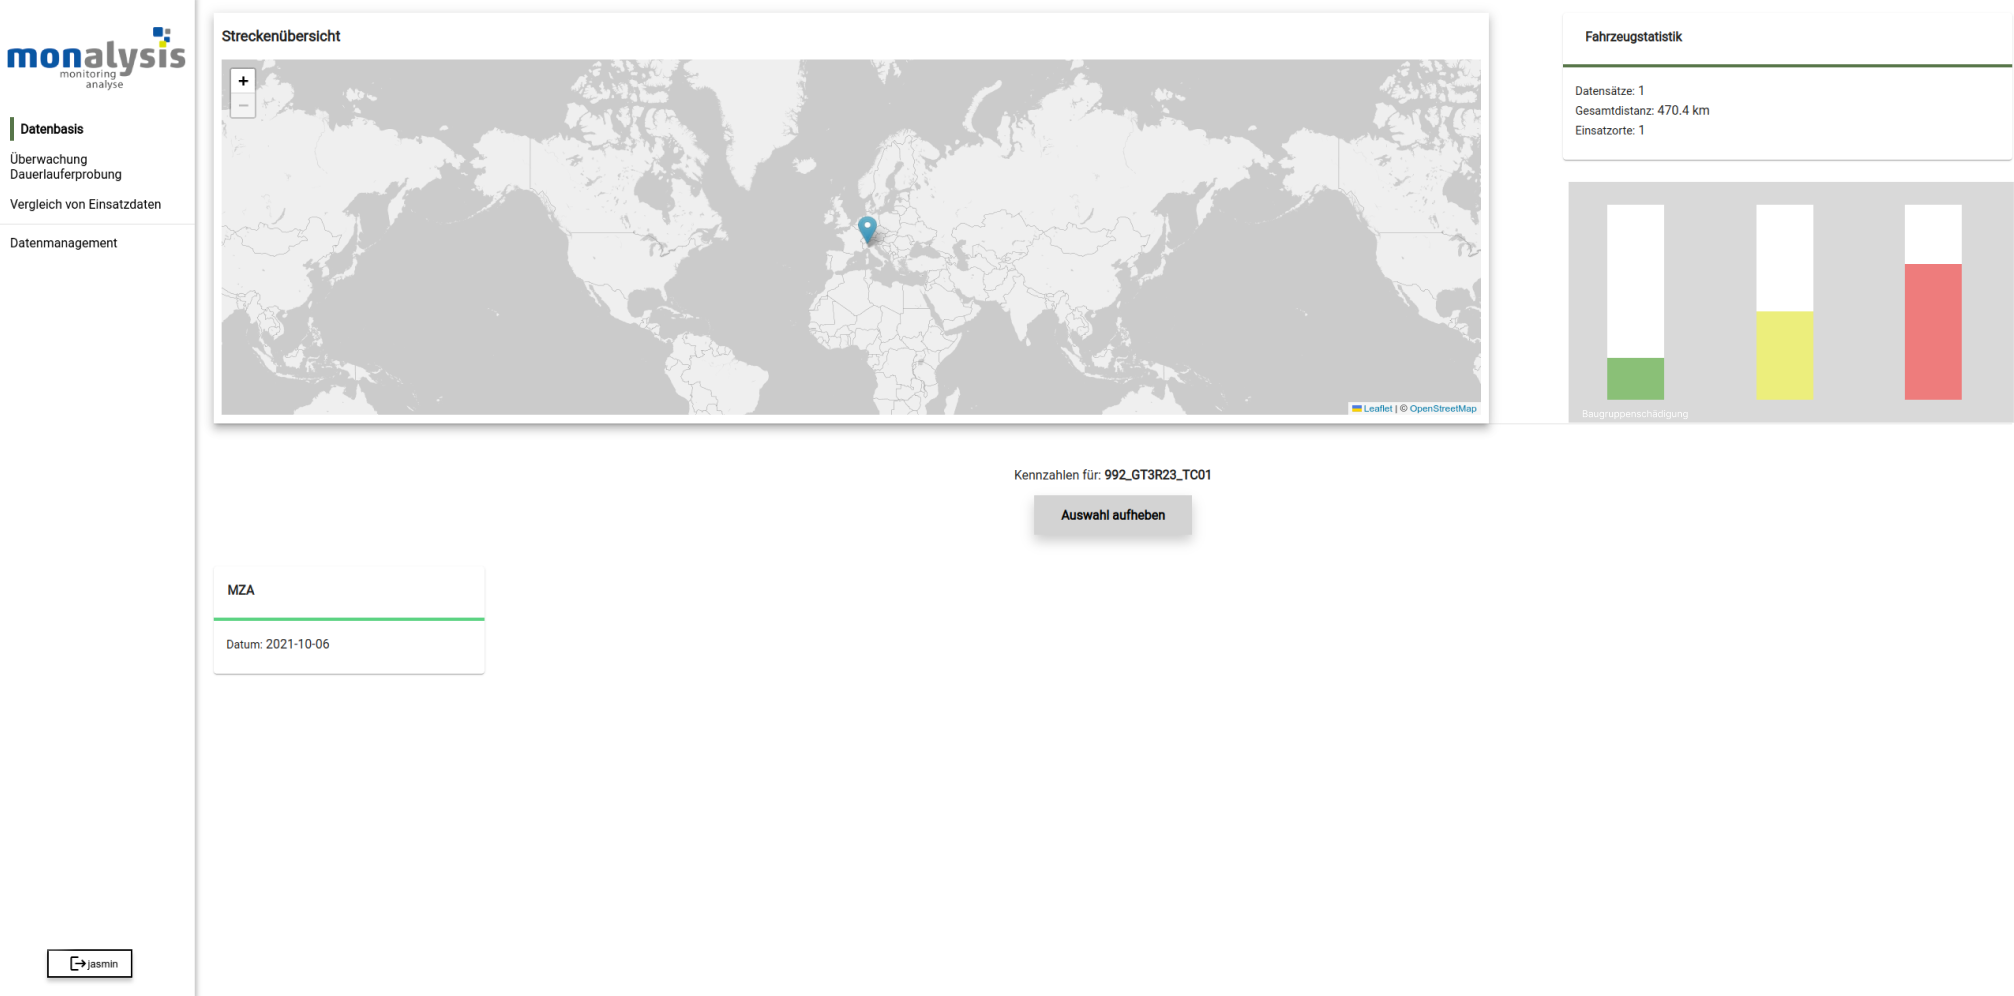
\includegraphics[width=0.8\textwidth]{gfx/Figma_Datenbasis.png}}
\caption{Figma-Entwurf für die Fahrzeugdarstellung der Datenbasis}
\label{fig:datenbasis}
\end{figure}
Die bewerteten Baugruppen werden pro Fahrzeug festgelegt als:
\begin{multicols}{2}
\begin{itemize}
    \item Gesamtfahrzeug
    \item Feder-Dämpfer-System Vorderachse
    \item Feder-Dämpfer-System Hinterachse
    \item Querlenker Vorderachse
    \item Querlenker Hinterachse
    \item Spurstange
    \item Lenkgetriebe
\end{itemize}
\end{multicols}
\noindent
Pro Baugruppe gibt es durch die Erprobung einen Grenzwert, ab dem die Baugruppe kritisch wird. Deshalb ist es sinnvoll, das Lastgeschehen als Prozentwert zu dem Grenzwert darzustellen. Bei der Zielgruppe dieses Graphen handelt es sich, wie bei allen Graphen, um Ingenieure, Maschinenbauer und Fahrzeugbauer. \\\\
2. Darstellung wählen:\\
Bei dieser Darstellung ist die Hauptinformation, wie das Lastgeschehen der einzelnen Baugruppen im Vergleich zu den erprobten Werten ist. Aus diesem Grund würden sich Gauge-Charts oder Bullet-Charts besonders gut eignen. Eine Gauge-Chart wird laut \cite{Schwabish.2021} typischerweise in einem Kreis oder Halbkreis dargestellt, dabei wird eine \glqq Nadel\grqq{} oder auch ein Pointer genutzt, um den aktuellen Wert auf einer Skala anzuzeigen. \cite{Schwabish.2021} beschreibt die Gauge-Chart als einen Graphen, der sich dazu eignet, eine generelle Auskunft über die Datenlage zu geben. Für mehr Details sollte aber eine andere Darstellungsart gewählt werden. Da bei dem aktuellen Fall relativ viele Baugruppenzustände dargestellt werden sollen und eine einzelne Gauge-Chart durch die runde Form zu viel Platz in Anspruch nimmt, sollte bei diesem Graphen eher eine Bullet-Chart gewählt werden. Bullet-Charts sind eine Weiterentwicklung der Gauge-Chart \cite{Schwabish.2021}. Generell sind Bullet-Charts lineare Versionen der radialen Gauge-Chart. Da die Bullet-Chart kompakt ist, eignet sie sich gut dafür, mehrere Werte übereinander darzustellen. \\\\
3. Ordnung schaffen:\\
Basierend auf dem Beispiel für eine Bullet-Chart von \cite{Plotly.2024c} wird zuerst eine Grundlage für die neue Chart geschaffen. Diese ist in Abbildung \ref{fig:bullet_chart_after} zu sehen.
Beim Ordnungschaffen geht es darum, nicht zwingend notwendige Bestandteile des Graphen zu entfernen. Zunächst wird das Delta unter den Zahlwerten entfernt, das Delta zeigt die Veränderung der Werte im Vergleich zu anderen Zeitpunkten. Bei diesem Usecase ist es aber kaum möglich, dass die Schädigung der Bauteile fällt, außer es werden Bauteile ausgetauscht, was die Schädigung dann aber auf den Wert null resetten würde. Es bietet sich auch an, den White Space zwischen den einzelnen Bullets zu erhöhen, um eine bessere Lesbarkeit der Legende zu erreichen. Eine weitere Möglichkeit wäre, eine Legende auf die gesamten Bullets zu beziehen, da die Werte in Prozent dargestellt werden sollen und dadurch immer den gleichen Wertebereich haben. Dadurch würde auch der Visual Clutter reduziert. Zudem wäre es möglich, die Werte, die \glqq zusammengehören\grqq{}, wie Querlenker Vorderachse und Querlenker Hinterachse, durch das Gestalt-Principle  \cite{Schwabish.2021} Connection, also Verbindungen, zu gruppieren. Die Schädigung soll in Prozent dargestellt werden, also bietet es sich auch an, beide Werte in einer gemeinsamen Bullet-Chart zusammenzufassen, da die beiden Querlenker auch dieselben Kriterien dafür haben, wann ein Prozentwert kritisch ist. Die Markierung für den Threshold kann ebenso entfernt werden. Auch die Nummer neben den Bullets kann entfernt werden, da es bei dieser Darstellung nicht um den genauen Wert geht, sondern eher um einen Überblick, wie es um das Fahrzeug steht. Deswegen können auch die Ticks entfernt werden. Mit den oben beschriebenen Änderungen kann der Graph auf Abbildung \ref{fig:bullet_chart_after} reduziert werden.\\\\
\begin{figure}
\centering
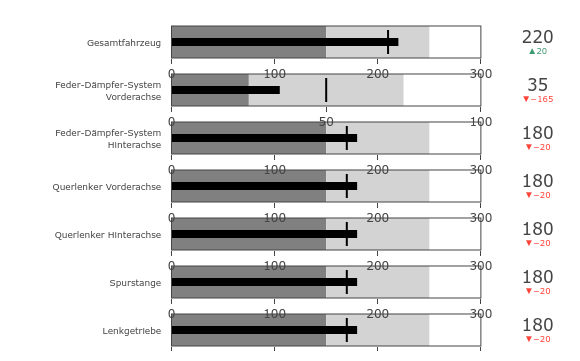
\includegraphics[width=.45\textwidth]{gfx/Bullet_Chart_Before.png} % Just stack two includegraphics!
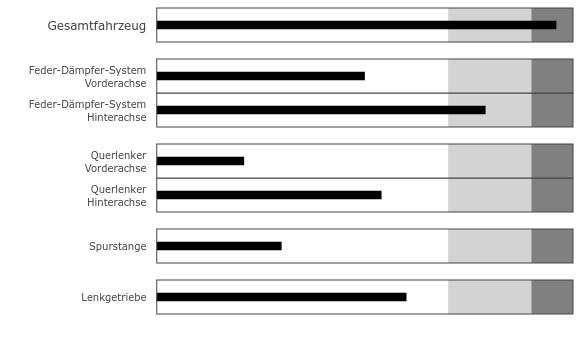
\includegraphics[width=.45\textwidth]{gfx/Bullet_Chart_After.png}
\caption{Bullet-Chart vor und nach dem Ordnungschaffen}
\label{fig:bullet_chart_after}
\end{figure}
4. Aufmerksamkeit bündeln:\\
Die Aufmerksamkeit des Benutzers soll bei dieser Darstellung auf die Bauteile gelenkt werden, die sich nah an den warnenden Zonen bei 70\,\% oder sogar an den kritischen Zonen der Schädigung der Bauteile bei 90\,\% befinden. Es bietet sich an, die bislang in verschiedenen Grautönen gehaltenen Steps je nach Status einzufärben. Als Farben wird für die kritischen Bereiche ein Pastellrot und für die Warnungsbereiche ein Pastellorange gewählt, für die nicht kritischen Bereiche ein Pastellgrün, um so bei dem Benutzer die Assoziation mit einer Ampel auszulösen. Da es sich bei den Benutzern um Ingenieure und Maschinenbauer handelt, ist davon auszugehen, dass diese Assoziation vom Gehirn schnell erzeugt werden kann. Bei den Farben wird darauf geachtet, dass diese auch auf einer Grauskala gut erkennbar sind. Auch der Wert des Gesamtfahrzeugs sollte herausstechen, dafür wird die Schriftgröße des Labels angepasst. Die Farbe des Values wird bei den anderen Gauges zu einem dunklen Grau angepasst.\\\\
5. Geschichte erzählen:\\
Als logischer Call to Action ergibt sich aus dem Graphen der Aufruf zur Wartung eines Fahrzeugs, falls Werte die pastellroten Bereiche des Graphen erreichen sollten, da nach der Schädigung im Ausmaß von 100\,\% nicht mehr davon ausgegangen werden kann, dass das Fahrzeugteil weiter einsatzfähig ist. Da sich der Graph im Layout der Seite eher im Hintergrund befindet, ist es empfehlenswert, diese wichtige Warnung an anderer Stelle einzublenden. Dafür eignet sich eine Position direkt unter der Karte, damit die Warnung in das Auge fällt. Die gewählte Aufteilung des Graphen ist zufälligerweise bereits in den vorherigen Graphen vorhanden. Das Gesamtfahrzeug sollte an erster Stelle stehen, da es sich bei dem Wert um die Summe aller anderen Werte handelt. Zudem wird ein dezenter Strich als Trennung des Gesamtfahrzeugs von den Werten der Fahrzeugkomponenten eingefügt, um zu verdeutlichen, dass das Fahrzeug der wichtigste Wert ist. Es gibt einen Titel, der angibt, was in welcher Einheit auf dem Graphen dargestellt wird.
\begin{figure}[h!]
\centering
\fbox{
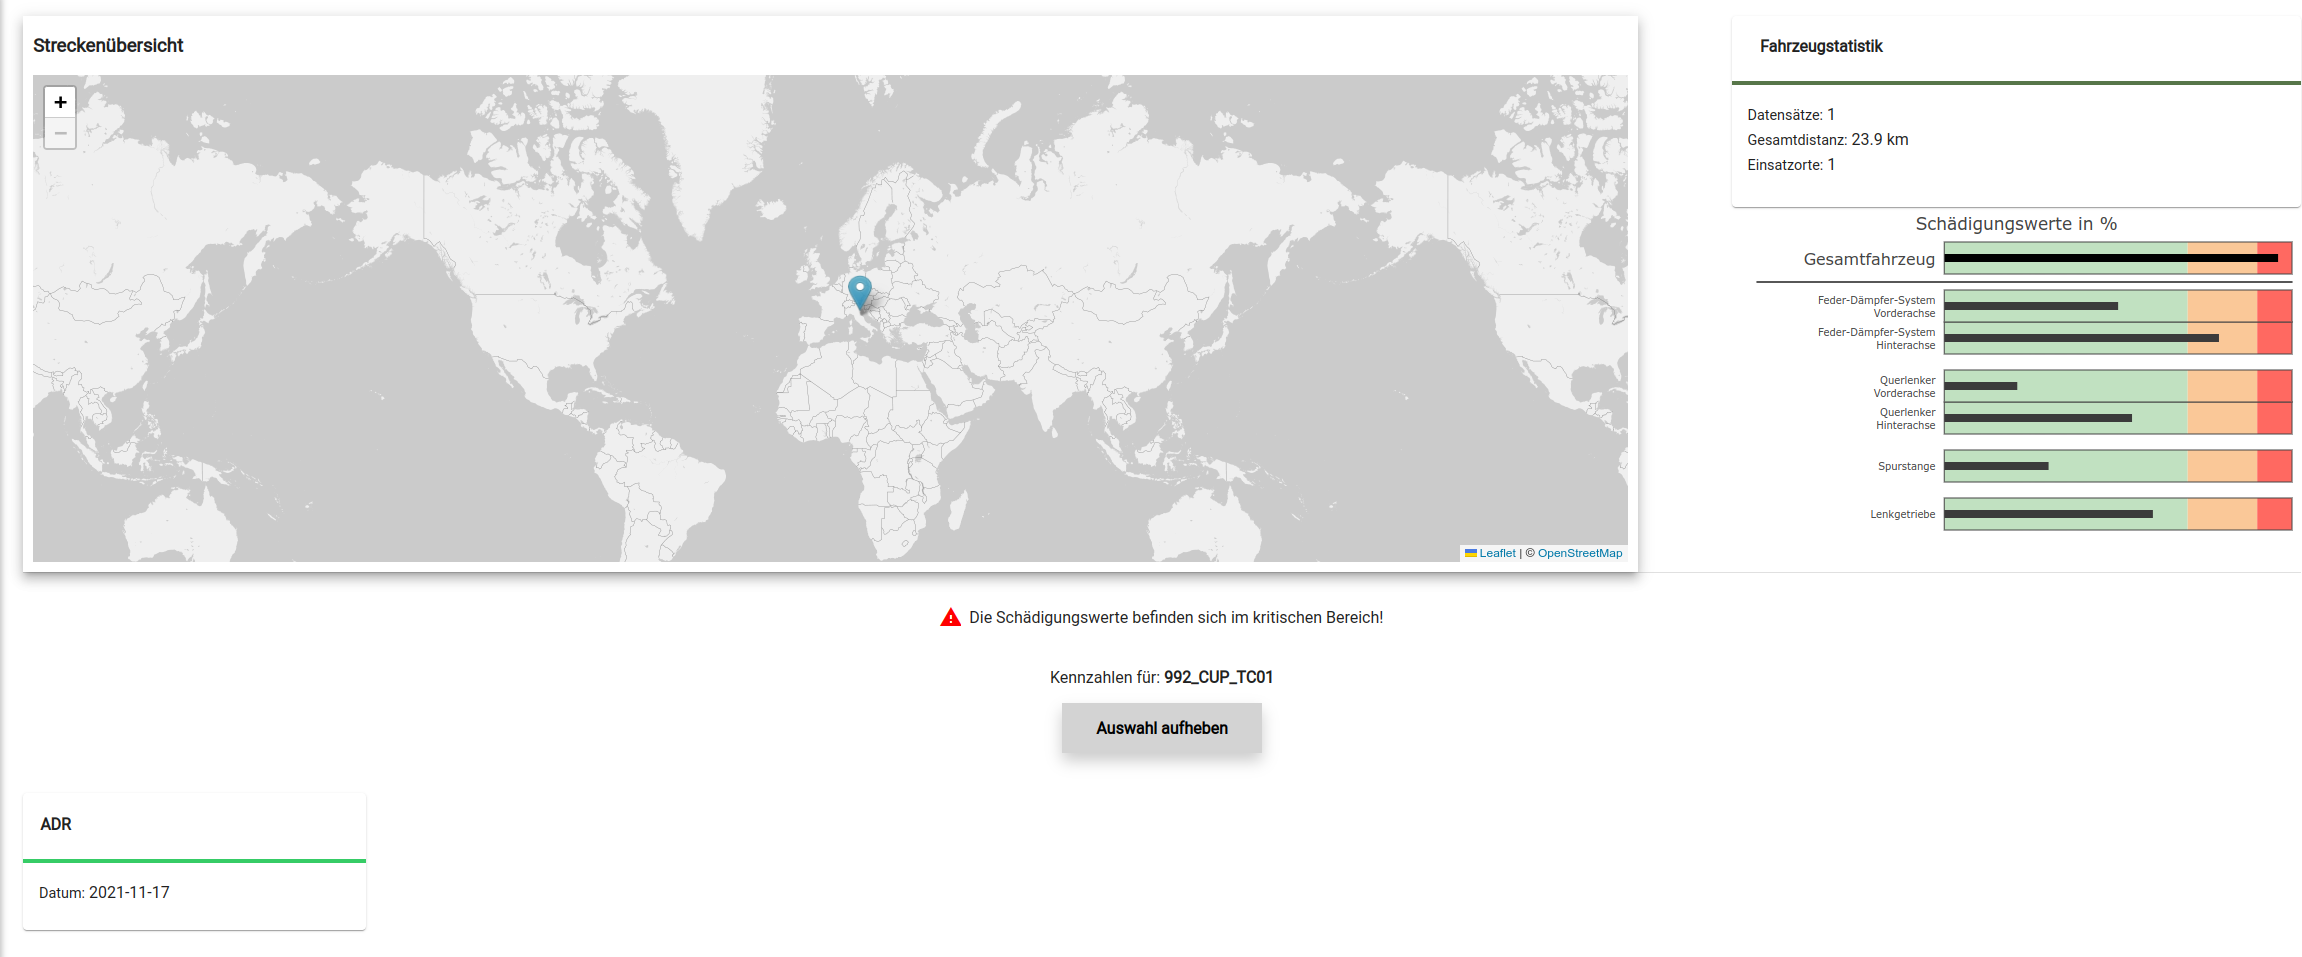
\includegraphics[width=0.8\textwidth]{gfx/Datenbasis_After.png}}
\caption{Datenbasis mit Bullet-Chart und Warnung}
\label{fig:datenbasis_after}
\end{figure}
\noindent
Nach Implementation des Graphen und der Warnung sieht die Datenbasis wie  in Abbildung \ref{fig:datenbasis_after} dargestellt aus.

\subsection{Fahrzeugvisualisierung mit Einfärbungen passend zur prozentualen Schädigung}
\label{sec:vehicle-images}
1. Kontext verstehen:\\
Um dem Benutzer zu ermöglichen, auch visuell zu erkennen, wo welche Schädigungen vorhanden sind, wird eine Fahrzeugvisualisierung eingebaut. Da es sich bei den zu überwachenden Fahrzeugen immer um das gleiche Modell handelt, ist die Implementation einfach gehalten. Es soll eine Möglichkeit gegeben werden, die einzelnen Konzeptzeichnungen der Fahrzeuge zu betrachten, wobei die Bauteile mit hoher Schädigung ähnlich wie in der Bullet-Chart in \ref{section:Prozentuale_Schädigung} eingefärbt werden sollen.\\\\
\begin{figure}[h!]
\centering
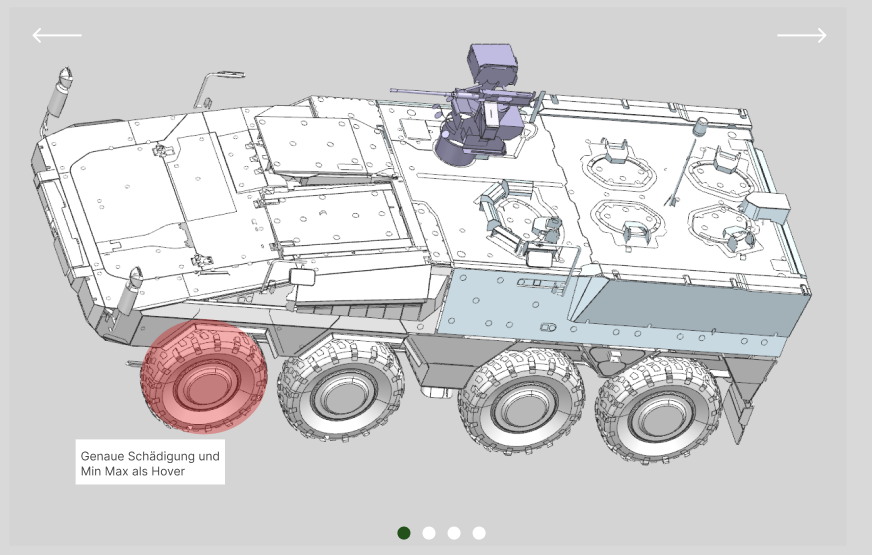
\includegraphics[width=0.8\textwidth]{gfx/vehicle_visualisation.png}
\caption{Prototyp der Fahrzeugvisualisierung}
\label{fig:vehicle_visualisation}
\end{figure}
\noindent
2. Darstellung wählen:\\
Als Darstellung eignet sich ein Karussell, in dem die Bilder angezeigt werden. Dann sollen die Bauteile eingefärbt werden und die Schädigung soll mit einem Hovereffekt mithilfe einer Image-Map ersichtlich werden. Bei dieser Darstellung handelt es sich zwar um keinen Graphen, Data-Storytelling kann aber trotzdem angewendet werden. Es wird in Figma \cite{FigmaGmbH.2024} ein Prototyp der Visualisierung erstellt (siehe Abbildung \ref{fig:vehicle_visualisation}).\\\\
3. Ordnung schaffen:\\
Um Ordnung zu schaffen, wird der Prototyp aus Figma \cite{FigmaGmbH.2024} dezenter implementiert. Dabei werden insbesondere als Pfeile zum Wechseln der Bilder solche gewählt, die weniger lang sind. Diese Pfeile werden in runde Buttons integriert. Bei der Darstellung, auf welchem Bild man sich im Karussell befindet, werden die Größe und die Farbe angepasst.\\\\
4. Aufmerksamkeit bündeln:\\
Die Aufmerksamkeit wird durch die farbigen Boxen auf der Image-Map gebündelt. Dabei wird anhand der Schädigung eine Farbe gewählt. Die Farben sind die gleichen wie in \ref{section:Prozentuale_Schädigung}, da auch in dieser Darstellung die Schädigung dargestellt wird. Es ist sinnvoll, die Farben über die gesamten Visualisierungen konstant zu halten, da der Benutzer in seinem Gehirn die Verbindung zwischen den Farben und dem Zustand der Schädigung herstellen wird. Mit dem Hovereffekt werden der Name der jeweiligen Komponente sowie die Schädigung angezeigt.\\\\
5. Geschichte erzählen:\\
Die Farben, die im Punkt 4. gewählt wurden, sowie die weiteren Graphen auf der Webseite dienen dazu, die Geschichte dieser Visualisierung zu erzählen. Analog ist der Call to Action bei \glqq roten\grqq{} Komponenten, diese zu warten oder zu erneuern. Die vollständige Visualisierung ist in Abbildung \ref{fig:vehicle_visualization_after} zu sehen. 
\begin{figure}[h!]
\centering
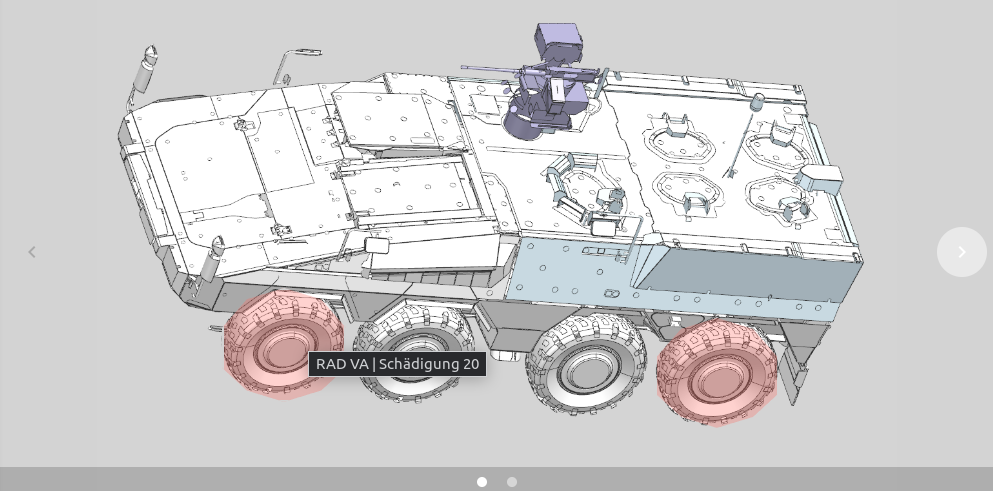
\includegraphics[width=0.8\textwidth]{gfx/vehicle_visualisation_after.png}
\caption{Fahrzeugvisualisierung der Baugruppen mit Hovereffekt}
\label{fig:vehicle_visualization_after}
\end{figure}
\noindent
Die Visualisierung ist in zwei verschiedene Arten von Bildern eingeteilt: zum einen die Bilder, die die Baugruppen des Fahrzeugs zeigen, und zum anderen die Bilder, die die einzelnen Komponenten in den jeweiligen Baugruppen darstellen. Es wird bei dieser Visualisierung also eine Art Drill-down genutzt, um die verschiedenen Komponenten darzustellen. Zunächst sind nur die Bilder der Baugruppen im Karussell zu sehen. Wird aber auf eine Baugruppe geklickt, wird ein weiteres Bild zum Karussell hinzugefügt und das Karussell zu der passenden Position navigiert. Dadurch lässt sich die Auswirkung der einzelnen Komponenten auf die Baugruppen wirkungsvoll darstellen. Da sich die Bilder bei Hinterachse und Vorderachse kaum unterscheiden, wurde zum einfacheren Verständnis ein Titel hinzugefügt. Die Komponentenbilder sind in Abbildung \ref{fig:vehicle_visualization_detail} dargestellt.
\begin{figure}[h!]
\centering
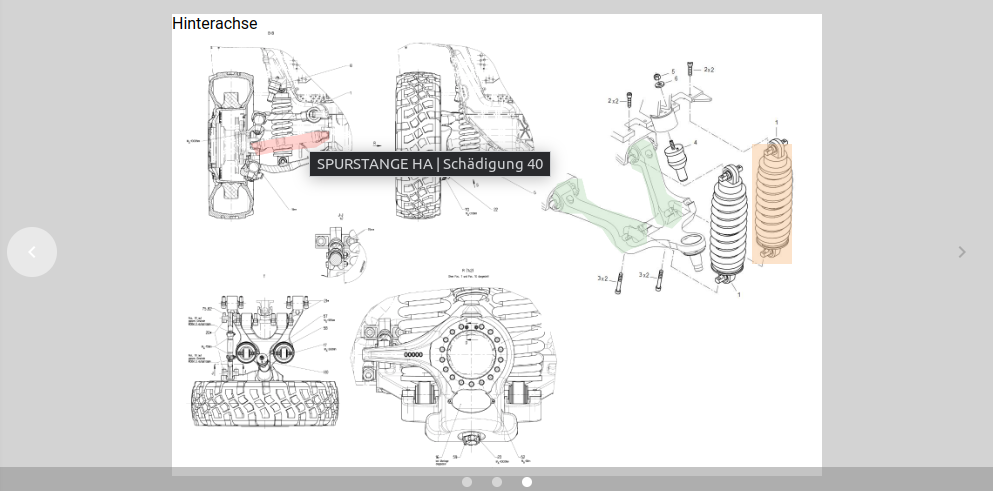
\includegraphics[width=.8\textwidth]{gfx/vehicle_visualisation_detail.png}
\caption{Fahrzeugvisualisierung der Komponenten mit Hovereffekt}
\label{fig:vehicle_visualization_detail}
\end{figure}
\subsection{Fingerprints}
1. Kontext verstehen:\\
Bei den von monalysis entwickelten Fingerprints \cite{MichaelStadele.2008} handelt es sich um eine Darstellung, die aus jeweils drei Teilen besteht. Dabei wird beschrieben, wie sich die Fahrbahn zum Bauteil verhält beziehungsweise wie belastend die Straßen sind. Außerdem können mit den Fingerprints Fahrmanöver erkannt werden \cite{MichaelStadele.2008}. Die drei Teile setzen sich zusammen aus aX, aY und aZ, die die verschiedenen Raumrichtungen beschreiben. Jede dieser Raumrichtungen hat wiederum Frequenzbänder, die dargestellt werden sollen. Insgesamt gibt es pro Raumrichtung neun Frequenzbänder in diesem Anwendungsfall. Die Frequenzbänder werden als aX1--aX9 bezeichnet, wobei gilt: Je niedriger die Zahl, desto niederfrequenter ist die Messung. Zusätzlich soll noch die gesamte Schädigung pro Raumrichtung dargestellt werden. Die Fingerprints wurden deswegen entwickelt, weil man alleine über die Schädigung keinen Überblick über die niederfrequenten Bereiche der Messung hat. Durch die Darstellung der Fingerprints wird die Intensität der Straße erkennbar.\\\\
2. Darstellung wählen:\\
Als Darstellung für die Fingerprints eignet sich eine Linechart. Die drei Raumrichtungen werden zwar separat betrachtet, aber es ist doch wichtig, die Verläufe vergleichen zu können. Für die Fingerprints ist bereits eine Implementation vorhanden, auf welcher der Graph basiert (\ref{fig:fingerprints_first}).
\begin{figure}[!h]
    \centering
    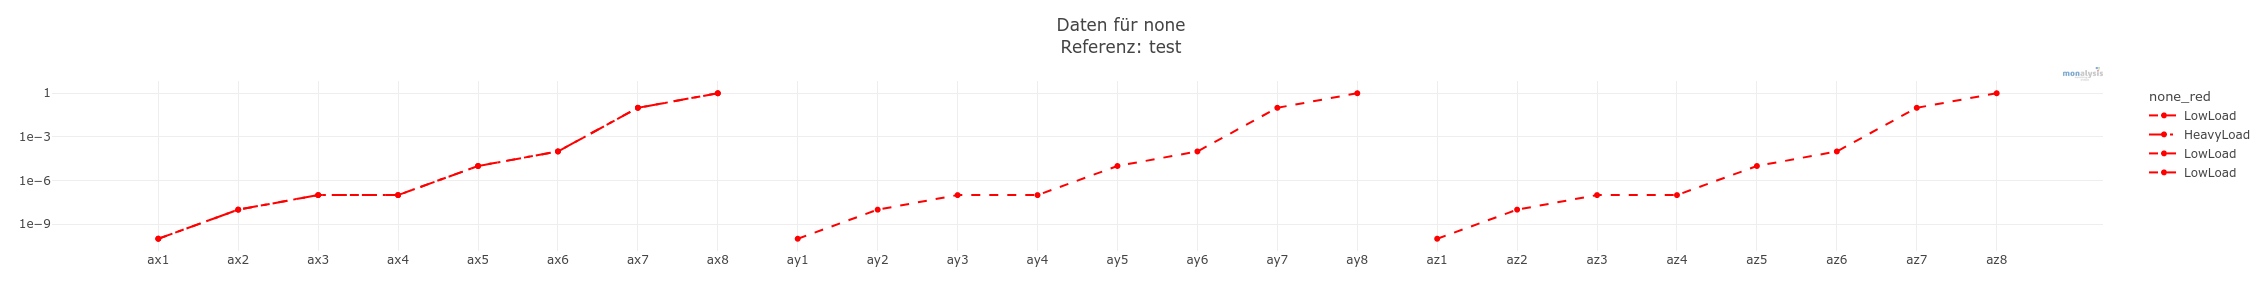
\includegraphics[width=1\linewidth]{gfx/fingerprints_first.png}
    \caption{Bereits vorhandene Implementation der Darstellung der Fingerprints}
    \label{fig:fingerprints_first}
\end{figure}
\\\\3. Ordnung schaffen:\\
Im Sinne des Data-Storytelling-Punkts „Ordnung schaffen“ ist die bereits vorhandene Implementierung gut gelungen. Bei den Gridlinien werden die vertikalen Linien für aX, aY und aZ entfernt. Ebenso wird der Titel des Graphen überarbeitet. Für diese Implementation ist weder eine Region noch eine Referenz vorgesehen, also kann der Titel entfernt werden. Die Implementation der Linien wird überarbeitet, sodass die Linien als einfache Linien dargestellt werden können, anstatt in verschiedene Richtungen unterbrochen. Das beruhigt den Graphen im Allgemeinen. Die Implementation wird weiterhin angepasst, sodass keine mehrfachen Einträge in der Legende sichtbar sind. Die Position des Logos ist in diesem Graphen gut gelungen, da weder die Daten noch das Logo überdeckt werden. Der Graph wird als zwei verschiedene Varianten implementiert: Es ist möglich, mehrere Fingerprints in einem Graphen darzustellen oder diese mit einem Toggle voneinander zu trennen und separate Graphen zu rendern. Zudem wird die Limitation festgelegt, dass nur fünf Fingerprints gleichzeitig dargestellt werden können.\\\\
4. Aufmerksamkeit bündeln:\\
Um die Aufmerksamkeit des Benutzers auf die einzelnen Raumrichtungen zu lenken, werden Annotations erstellt, die den im Punkt „Ordnung schaffen“ entfernten Titel ersetzen. In der Legende wird der erzeugte Name des Fingerprints dargestellt, der sich aus Fahrzeugname, Erprobungsbahn, gefahrener Geschwindigkeit und Laufleistung zusammensetzt. Dadurch sieht man auf einen Blick, welche Parameter für die Linie wichtig sind. Ansonsten sollen die Linien farbig gekennzeichnet werden. Da es sich um bis zu fünf Linien handeln kann und diese nur durch ihre Farben zu unterscheiden sind, werden die klassischen Farben Rot, Grün, Blau, Schwarz und Grau gewählt. Wird ein einzelner Fingerprint dargestellt, soll dieser im gleichen Grau gefärbt werden wie die Zeitreihen \ref{sec:timeseries}.\\\\
5. Geschichte erzählen:\\
Die Fingerprints sind ein Analysewerkzeug, bei dem es relevant ist, wie nah die gemessenen Daten an der Zahl Eins sind, also wie nah die ausgewählte Messstelle sich an 100\,\% Erprobung befindet. Dazu wird das Grid bei der Zahl Eins hervorgehoben. Dadurch kann der Benutzer direkt erkennen, wie nah sich die Messstelle der Erprobung nähert, und somit auch abschätzen, wann diese Messstelle potenziell ausgetauscht oder gewartet werden soll. Mit diesen Anpassungen wird die Fingerprintdarstellung in \ref{fig:fingerprints_finished} abgebildet.
\begin{figure}[!h]
    \centering
    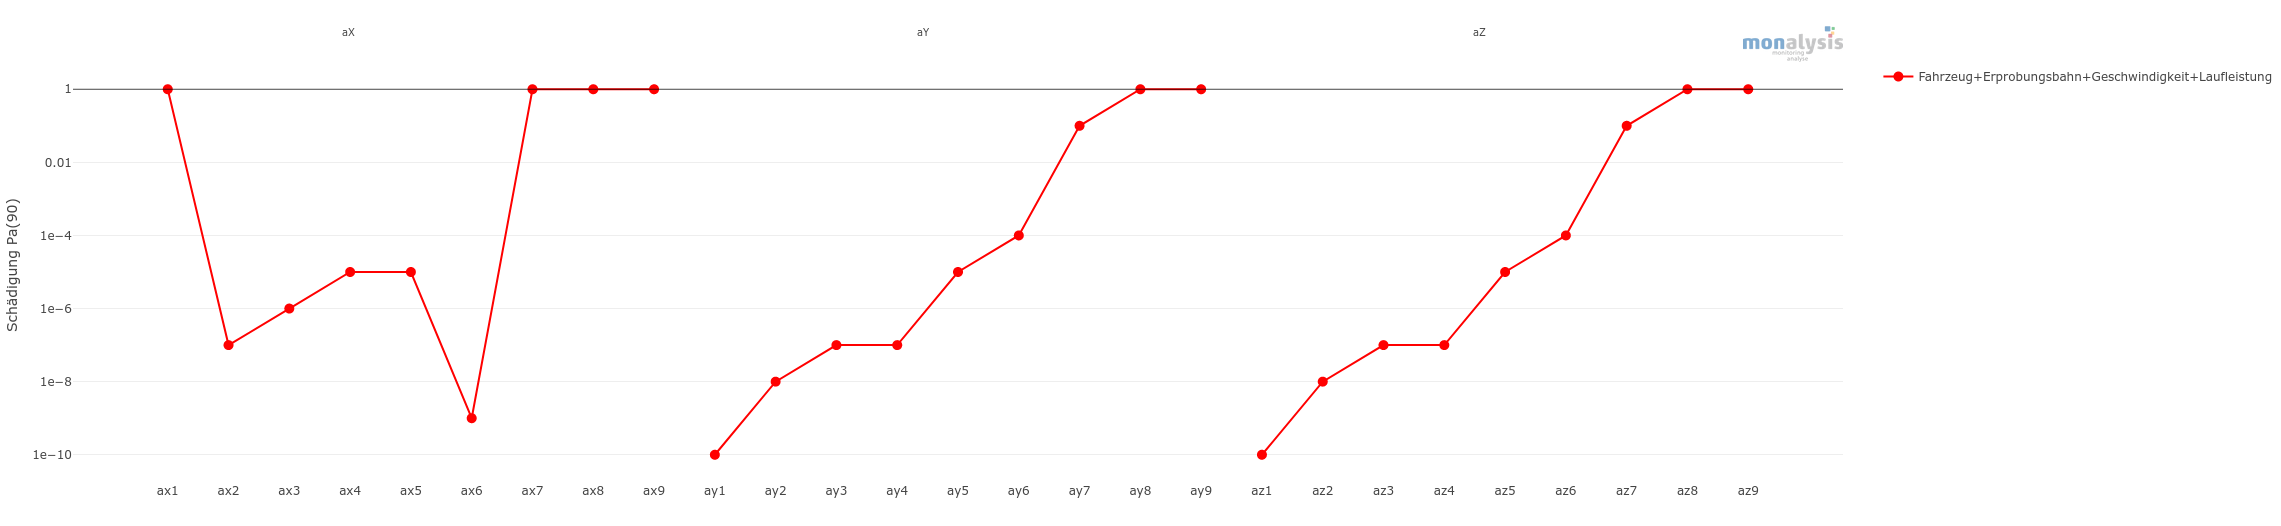
\includegraphics[width=1\linewidth]{gfx/fingerprints_finished.png}
    \caption{Vollständige Darstellung der Fingerprints}
    \label{fig:fingerprints_finished}
\end{figure}
\subsection{Dauerlauferprobung}
\label{section:dauerlauferprobung}
1. Kontext verstehen:\\
Die Dauerlauferprobung soll ein Graph sein, der die Schädigung über die Zeit (oder die bereits gefahrenen Kilometer) der Erprobung darstellt, zudem die Grenze, ab der die betrachtete Messstelle oder das Gesamtfahrzeug nicht mehr erprobt ist. Die Dauerlauferprobung ist also eine Ansammlung von Werten über einen Zeitraum und dazu eine spezifische Grenze. Es gibt für die Dauerlauferprobung zwei verschiedene Anzeigen: eine, die in einem Graphen die gesamte kumulierte Schädigung anzeigt, und eine, die sich auf die unterschiedlichen Raumrichtungen aX, aY und aZ beschränkt. Im Folgenden wird der Graph für die gesamte kumulierte Schädigung betrachtet. Es soll möglich sein, bei der x-Achse umzustellen, ob die Zeit betrachtet wird oder die gefahrenen Kilometer. Insgesamt sind in einer Dauerlauferprobung bei diesem Anwendungsfall immer 16\,000\,km zu fahren.\\\\
2. Darstellung wählen:\\
Es bietet sich an, den Graphen als einen Linegraphen zu implementieren, da es sich um eine Ansammlung von Werten über die Zeit handelt. Dadurch lässt sich auch die Grenze der Erprobung gut hervorheben.\\\\
 3. Ordnung schaffen:\\
Es wird bei der Erstellung des Graphen von dem plotly.js-Beispiel für einen Linegraphen ausgegangen \cite{Plotly.2024}. Da bei dieser Darstellung das Interesse bei dem Verlauf sowie dem aktuellen Stand der Dauerlauferprobung liegt, bietet es sich an, die Range des Graphen zu erhöhen, damit der aktuelle Zeitpunkt zentrierter im Graph ist und mehr hervorgehoben wird. Zusätzlich wird ein Titel hinzugefügt, damit der Benutzer direkt weiß, was dieser Graph darstellt. Da der Wert der Messung im Vordergrund steht, wird, um den Visual Clutter zu entfernen, das Grid für die x-Werte entfernt. Der Graph vor und nach dem Ordnungschaffen ist in Abbildung \ref{fig:dauerlauferprobung_before} dargestellt.
\begin{figure}[!h]
    \centering
    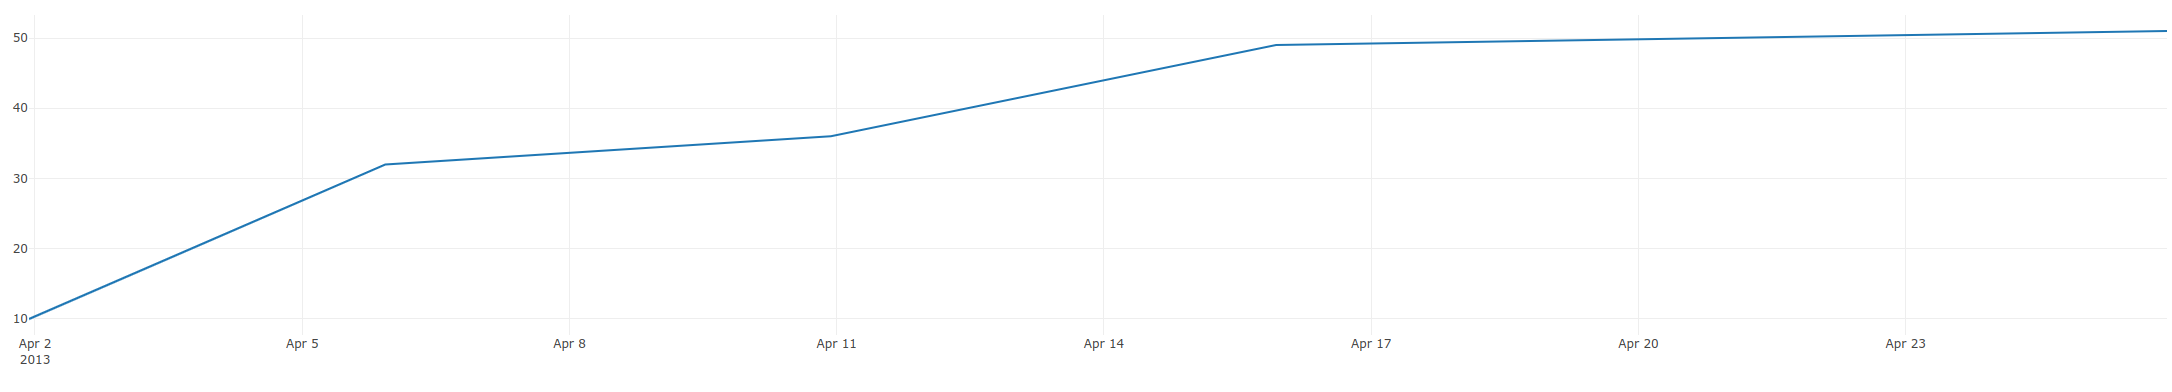
\includegraphics[width=\linewidth]{gfx/dauerlauferprobung_before.png}
        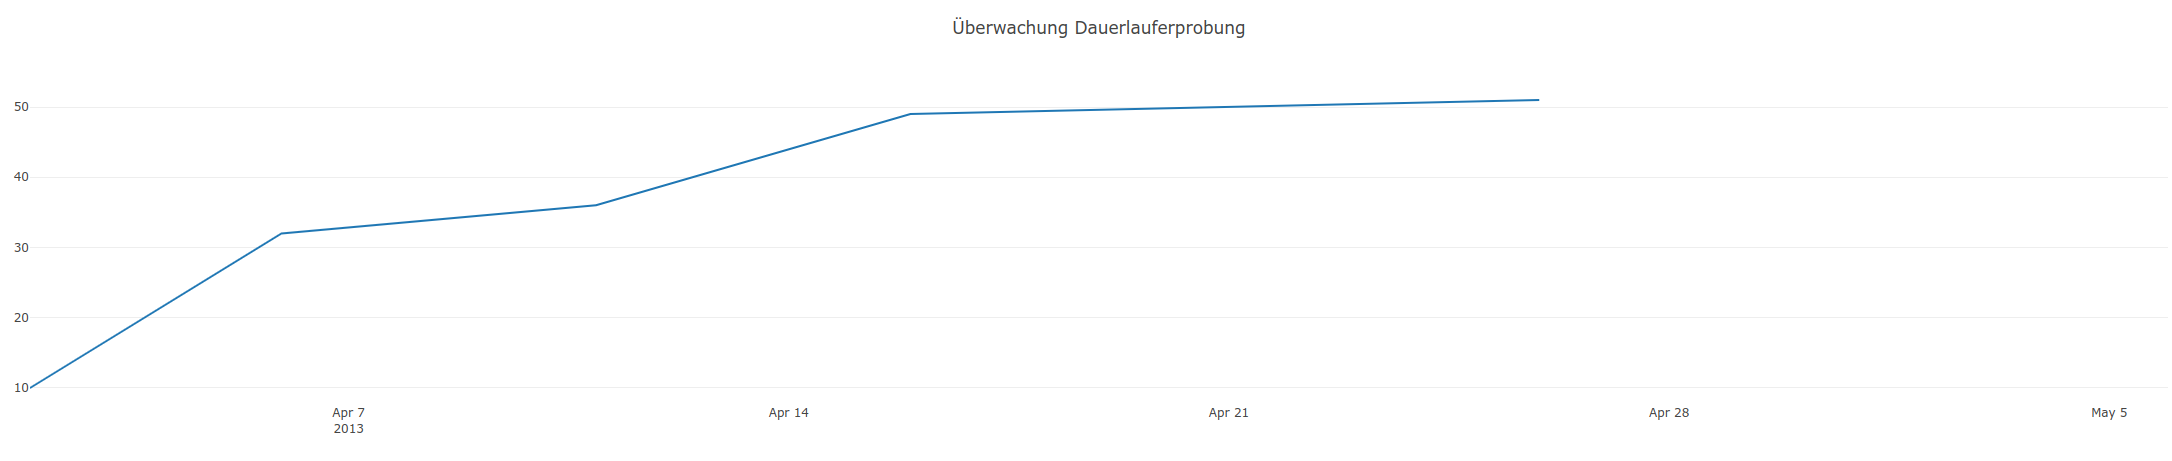
\includegraphics[width=1\linewidth]{gfx/dauerlauferprobung-after.png}
    \caption{Dauerlauferprobung vor und nach dem Ordnungschaffen}
    \label{fig:dauerlauferprobung_before}
\end{figure}
\\\\
 4. Aufmerksamkeit bündeln:\\
Sinnvoll ist es, den Wert der Grenze in dem Graphen darzustellen. Dadurch wird die Aufmerksamkeit des Benutzers nicht nur gebündelt, sondern der Benutzer kann direkt erkennen, wie weit das Bauteil schon erprobt ist. Durch den bereits vorhandenen Verlauf des tatsächlichen Schadens kann der Benutzer auch ungefähr abschätzen, wann die Grenze überschritten werden könnte. Die Messungen können zwar in unregelmäßigen Abständen durchgeführt werden, aber es kann davon ausgegangen werden, dass sich die Schädigung pro Prüfung ungefähr gleich verhält. Die Linie des Graphen wird zusätzlich passend zu den weiteren Graphen auf der Webseite eingefärbt. Das Ergebnis ist in Abbildung \ref{fig:dauerlauferprobung_aufmerksamkeit} abgebildet.
\begin{figure}[!h]
    \centering
    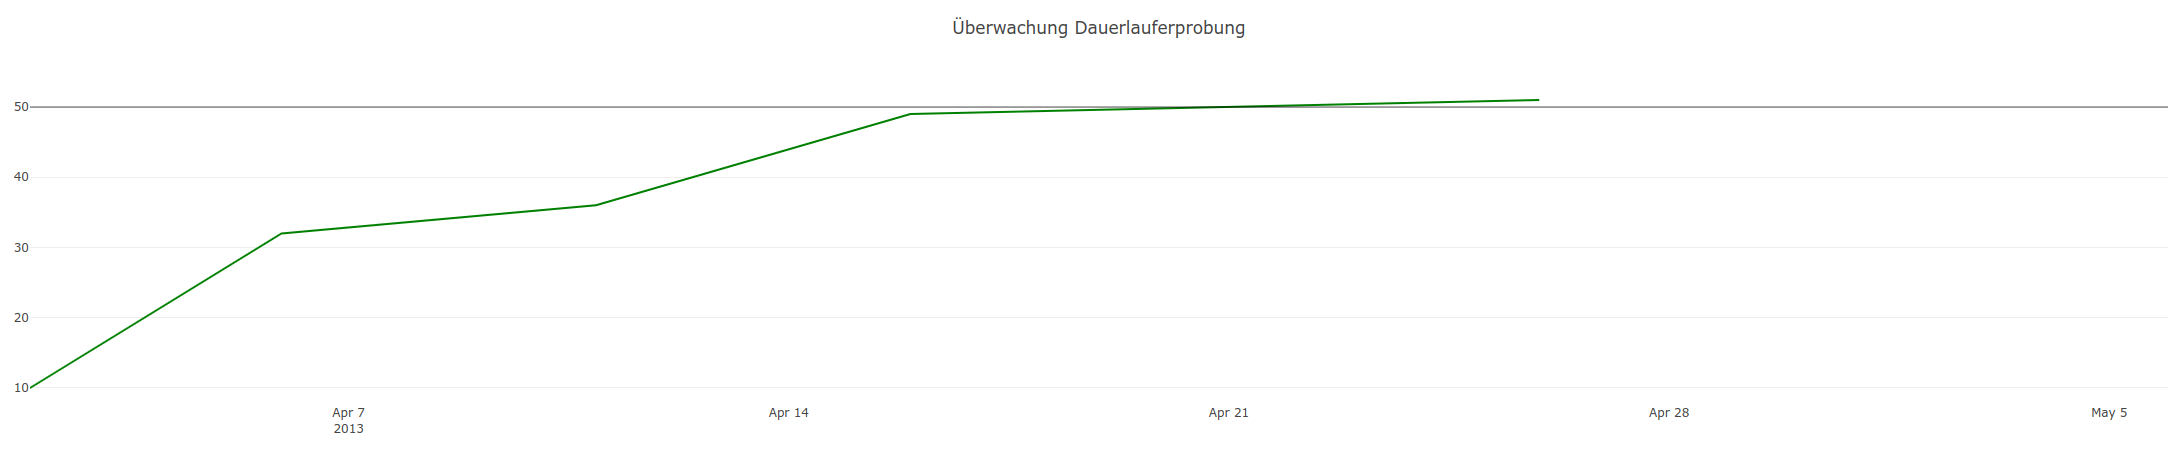
\includegraphics[width=1\linewidth]{gfx/dauerlauferprobung_aufmerksamkeit.png}
    \caption{Dauerlauferprobung mit eingezeichneter Grenze und passender Farbe}
    \label{fig:dauerlauferprobung_aufmerksamkeit}
\end{figure}
\\\\
 5. Geschichte erzählen:\\
Wichtig ist bei der Dauerlauferprobung zum einen, wann der tatsächliche Schaden die erprobte Grenze überschreitet. Zum anderen ist interessant, wann eine hohe Steigung in dem Verlauf der Erprobung erreicht wird. Wenn die erprobte Grenze überschritten wird, wird der Schnittpunkt der erprobten Linie und der Schäden gesucht. Deswegen ist es sinnvoll, diesen durch die Unterlegung von Farbe hervorzuheben. In plotly.js gibt es keine eingebaute Funktion, um den Schnittpunkt von zwei Linien herauszufinden. Aber da sich die Linie der Erprobung konstant auf einer Höhe befindet, kann man prüfen, wann diese Höhe überschritten wird, und den Punkt nach der Überschreitung und den Punkt vor der Überschreitung als Grenzen für die Einfärbung nutzen. Die Darstellung, wenn die Grenze überschritten wird, ist in Abbildung \ref{fig:dauerlauferprobung_story} zu sehen. Für das Erreichen einer gewissen Steigung kann die Trenderkennung genutzt werden. Die Werte der Dauerlauferprobung werden immer ansteigen, weil ein Fahrzeug keine negativen Kilometer zurücklegen kann. Also eignet sich die Funktion zum Erkennen der Aufstiege \texttt{detectRisesInData} aus \ref{subsection:risesAndFalls}, wobei eine Distanz von 0 zwischen dem Start- und Endpunkt angegeben wird. Auch der gleitende Durchschnitt ist für diesen Anwendungsfall nicht unbedingt nötig, da keine kleinen Abstiege ausgeglichen werden müssen. Als Eingabe für den gleitenden Durchschnitt bei der Funktion können auch einfach die richtigen Werte aus der Dauerlauferprobung weitergegeben werden.\\\\
\begin{figure}[!h]
    \centering
    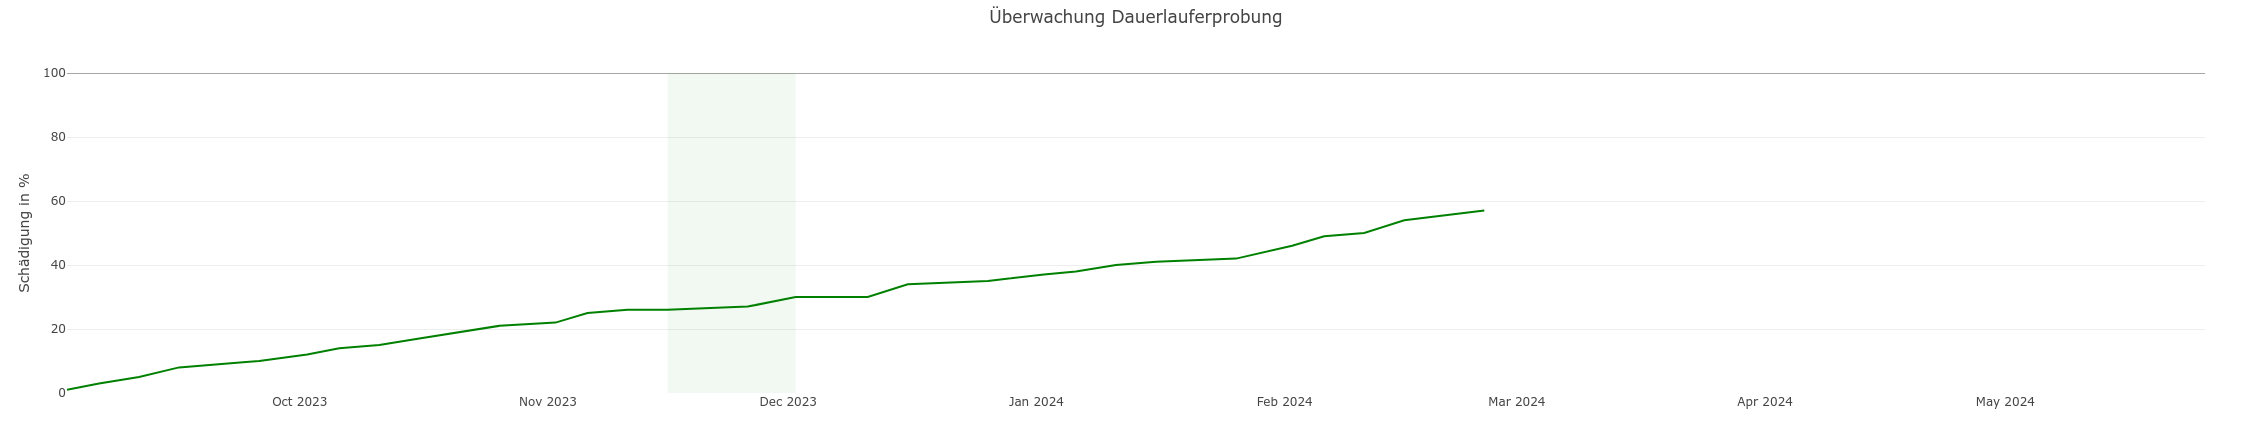
\includegraphics[width=1\linewidth]{gfx/dauerlauferprobung_story.png}
    \caption{Dauerlauferprobung mit den erkannten Aufstiegen}
    \label{fig:dauerlauferprobung_story}
\end{figure}

\subsection{Kumulierte Schädigung von allen gemessenen Durchfahrten}
\label{section:schaedigung}
1. Kontext verstehen:\\
Dieser Graph soll als Einstiegspunkt für die Analysen gelten. Es soll eine Übersicht über die verschiedenen gefahrenen Runden in den Daten geben. Dabei sollen pro gemessener Fahrt jeweils die Minimal-, Maximal- und Schädigungswerte der Messstellen dargestellt werden. Der Graph soll eine Bar-Chart sein, damit die verschiedenen Größen untereinander verglichen werden können. Die Balken sollen horizontal angeordnet sein. Ein Fahrzeug kann bis zu 50 Messstellen haben. Die Daten für diesen Graphen werden als Typ \texttt{ProfileData} aus \ref{appendix:graph_types} formatiert. 
\\\\
2. Darstellung wählen:\\
Ein Requirement für den Graphen ist, dass die Darstellung in einem Balkendiagramm erfolgen soll. Das Diagramm soll die Balken von links nach rechts anordnen. Dadurch kann bei der Betrachtung direkt verglichen werden, wie die einzelnen Messstellen zueinander stehen. Hierbei können sogleich zu hohe Werte erkannt werden.\\\\
3. Ordnung schaffen:\\
Dieser Graph basiert auf einer bereits vorhandenen Implementation der Darstellung. Diese Implementation ist in Abbildung \ref{fig:schaedigung_before} zu sehen.
\begin{figure}[!h]
    \centering
    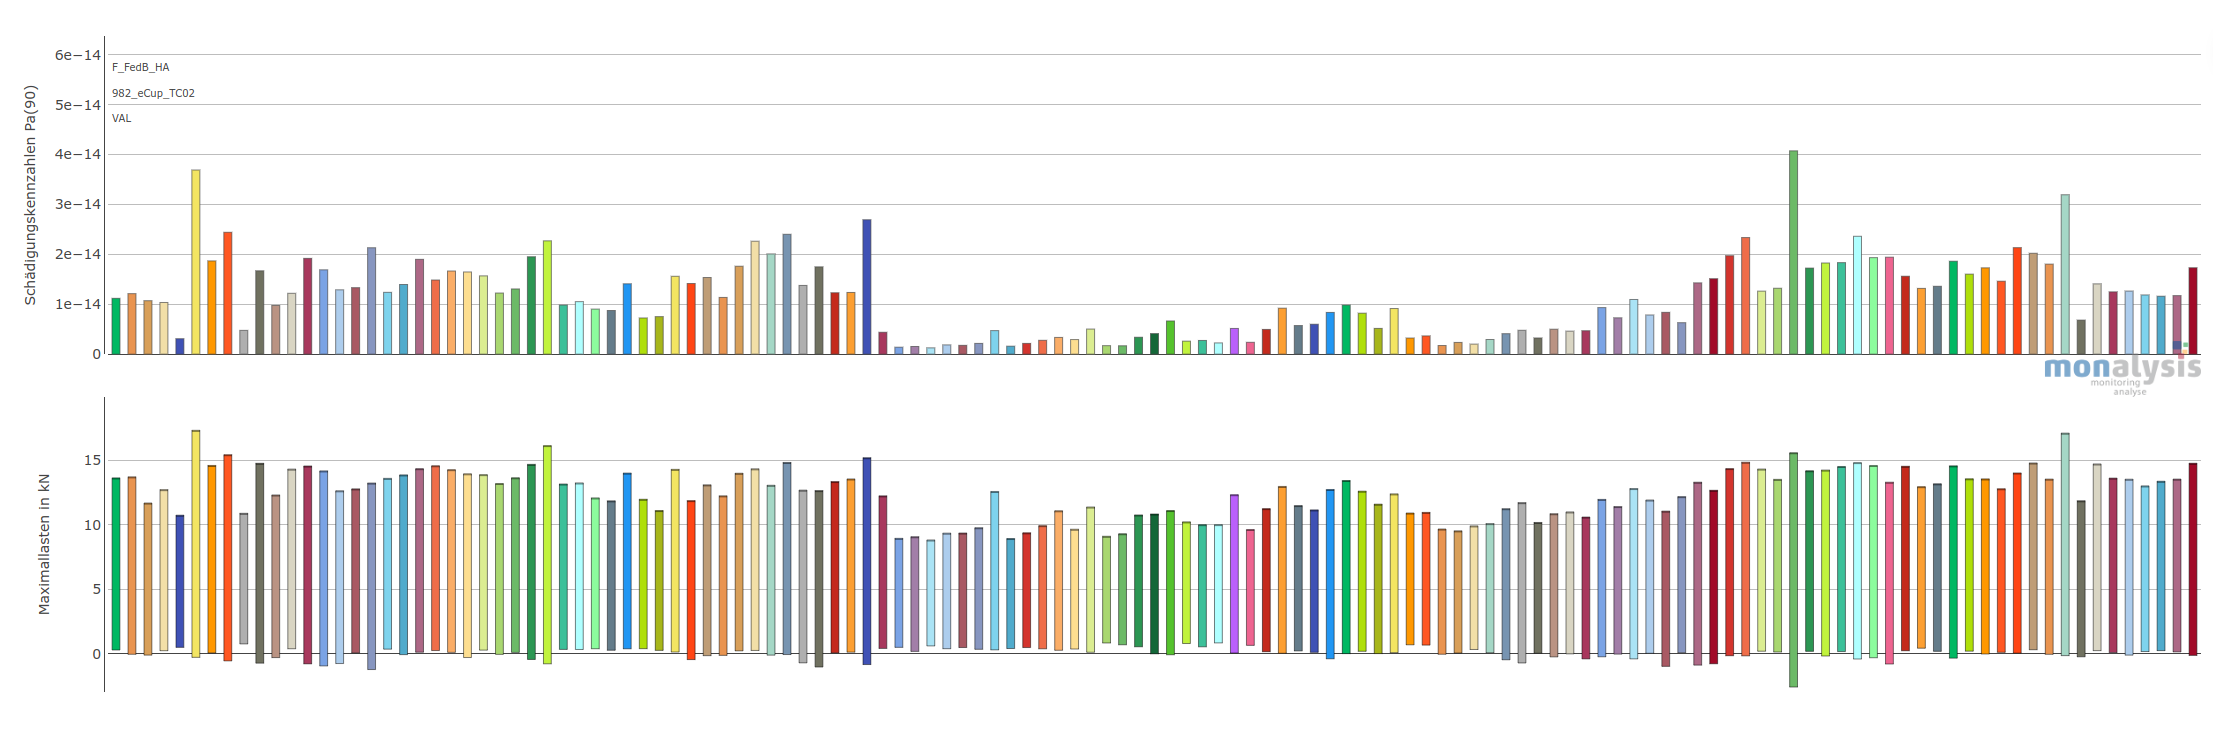
\includegraphics[width=1\linewidth]{gfx/schaedigung.png}
    \caption{Darstellung vor dem Data-Storytelling}
    \label{fig:schaedigung_before}
\end{figure}
Dadurch, dass in dem Graphen potenziell viele Messstellen dargestellt werden müssen, ist es umso wichtiger, die bisherige Darstellung zu vereinfachen. Zunächst werden die Farben aus den Balken entfernt, da laut \cite{BO.2019} Farben, je nachdem wie hell oder dunkel, ob es sich beispielsweise also um Grün oder Gelb handelt, unterschiedliche Effekte auf das Gehirn haben. So unterscheiden sich beispielsweise Grün oder Blau von den wärmeren Farben wie Rot oder Orange \cite{BO.2019}, da diese eher die Aufmerksamkeit des Benutzers auf sich ziehen. Da die Farben aber ursprünglich zufällig zugeordnet werden, kann nicht kontrolliert werden, welchen Balken warme und welchen kühle Farben zugewiesen werden. Deswegen werden in dieser Implementation die Balkenfarben entweder in einem einfachen Grau gehalten oder es können mithilfe eines zufälligen Grautongenerators verschiedene Grautöne generiert werden. In der Implementation ist ein Generator vorhanden, der auf \cite{Moob.2017} basiert, aber durch die Menge der darzustellenden Werte ist zunächst die Variante mit einem gleichen Farbton implementiert worden. Die Achsen haben bereits ein vereinfachtes Design; wenn zusätzlich die horizontalen Gridlinien entfernt werden, fällt das Vergleichen der Höhe der Balken schwerer. Das Logo der Firma sollte neu platziert werden, damit keine Balken überschnitten werden können. Auch die Platzierung der Achsentexte, \glqq Schädigungskennzahlen Pa(90)\grqq{} und \glqq Maximallasten in kN\grqq{}, werden durch die automatische Platzierung von plotly.js nicht genau untereinander gesetzt. Deswegen werden die Achsentexte durch Annotations ersetzt, die den gleichen Text darstellen, aber nicht abhängig von den Werten in der Achse platziert werden.\\\\
4. Aufmerksamkeit bündeln:\\
Aus den Experteninterviews konnte kombiniert werden, dass bei diesem Graphen hauptsächlich ein grober Überblick über die Daten und deren Beschaffenheit geschaffen werden soll. Zudem achten die Experten auf besonders hohe Balken, sowohl bei der Schädigung als auch bei den Minimal- und Maximalwerten. Es gibt dafür den internen Begriff „Topfilter“. Bisher wurde dieser Topfilter wie eine Auswahl gestaltet, bei der der Benutzer auswählen kann, wie viele Top-Werte dargestellt werden sollen. Dabei gibt es die Auswahlmöglichkeiten 1, 3, 5 und 10. Diese Top-Werte beziehen sich auf die Schädigungswerte. Sollten der  minimale und maximale Wert nicht unter den Top-Werten sein, werden diese zusätzlich hinzugefügt. Es werden also maximal 12 Werte als Top-Werte klassifiziert. Um die Aufmerksamkeit des Benutzers direkt auf die Top-Werte zu lenken, die laut den Experten der interessanteste Aspekt in der Darstellung sind, sollten die ersten Top-Werte gekennzeichnet werden, ohne dass der Benutzer eine Auswahl treffen müsste. Es bietet sich an, die Top-Werte einzufärben, da der Graph nun keine Farben mehr darstellt. Durch die Farbe fällt auf, welcher Wert für die Analyse interessant ist. Die Top-Werte lassen sich je nach Schädigung sortieren, und anhand dieser Sortierung wird der Farbton gewählt. Je heller die Farbe, desto höher die Schädigung, was in Kombination mit den grauen Balken der nicht als Top-Werte klassifizierten Werte zu einem Herausstechen der Top-Werte führt.
\begin{figure}[!h]
    \centering
    \includegraphics[width=1\linewidth]{gfx/schädigung_agter.png}
    \caption{Schädigungsdarstellung nach dem Ordnungschaffen und Aufmerksamkeitbündeln}
    \label{fig:schaedigung_after}
\end{figure}
\noindent
Dieser Effekt ist deutlich in Abbildung \ref{fig:schaedigung_after} zu betrachten. Es soll trotzdem noch die Möglichkeit gegeben sein, die Balken im Graphen auf die Top-Werte zu reduzieren. Durch diese Reduzierung kann der Benutzer die einzelnen interessanten Kanäle betrachten. Diese Reduzierung vom gleichen Datensatz ist in Abbildung \ref{fig:schädigung_reduziert} dargestellt. Da bei der Reduzierung nur maximal 12 Werte dargestellt werden, ist es möglich, bei der Darstellung einige Informationen hinzuzufügen. Die genauen Schädigungswerte werden auf den Balken eingeblendet, damit zu erkennen ist, welche Schädigungszahlen betrachtet werden. In plotly.js lässt sich für diesen Text nur eine Farbe angeben. Wenn die Balken aber beispielsweise dunkelgrün sind, ist schwarze Schrift nur schwer zu erkennen. Dafür wurde mithilfe von \cite{Alnitak.2012} eine Funktion entwickelt, die den Schädigungstext je nach Farbe des Balkens einfärbt. Wenn es weißer Text wird, wird bei diesem ein schwarzer Rand hinzugefügt.
\begin{figure}[!h]
    \centering
    \includegraphics[width=1\linewidth]{gfx/schädigung_reduziert.png}
    \caption{Reduzierung des gleichen Datensatzes wie in Abbildung \ref{fig:schaedigung_after}}
    \label{fig:schädigung_reduziert}
\end{figure}
\\\\5. Geschichte erzählen:\\
Der Graph erzählt die Geschichte, wie die verschiedenen Messungen auf den Messstellen ausgewertet wurden. Dabei ist das Erzählen einer Geschichte  schwierig, weil keine Messung als schlecht oder gut gelten kann, nur als interessant. Durch die farbliche Hervorhebung des Top-Wertes wird in gewisser Weise die Geschichte erzählt, da dieser Wert der interessanteste ist. Auch ein Call to Action ist so weit definierbar, dass die farbliche Hervorhebung dazu einlädt, die weiteren Funktionen zu nutzen. Damit kann analysiert werden, weshalb bei dieser Messung der höchste Wert aufgetreten ist. Dafür können über den Graphen durch einen Klick auf den Balken sowohl die Kollektive als auch die Zeitreihen angefordert werden. Die Kollektive eignen sich durch ihre unveränderliche Darstellung in der Betriebsfestigkeit \cite{Gotz.2020} und ihre Natur in der einfachen Darstellung von Ausschlägen in einem Messsignal \cite{PatrickPfeiffer.17.10.2022}  wenig zum Data-Storytelling, da es keinen Call to Action und auch keine Geschichte gibt, außer den Verlauf des Graphen. Die Zeitreihen hingegen eignen sich durch die Trenderkennung hervorragend für das Data-Storytelling.
% \subsection{Kollektive}
% 1. Kontext verstehen:\\
% Kollektive sind eine feste Größe in der Betriebsfestigkeit \cite{Gotz.2020}. Bei den Kollektiven werden laut \cite{PatrickPfeiffer.17.10.2022} lediglich die höchsten Ausschläge des Messsignals betrachtet. Dabei werden verschiedene Zählmethoden verwendet. In diesem Use Case gibt es die folgenden Darstellungen:
% \begin{description}
%   \item[Level Crossing (deut. Klassengrenzenüberschreitungszählung)] \hfill \\ 
%   Das Level Crossing Verfahren \glqq beschreibt die Häufigkeit, mit welcher die Last-Zeit-Funktion [(Zeitreihe oder Messung)] zuvor definierte Klassen überschreitet. [Deswegen] kann ein schneller Überblick über gemessene Minima und Maxima gewonnen werden\grqq{} \cite{PatrickPfeiffer.17.10.2022} \cite{TaylanKaplan.01.04.2015}.
%   \item[Range Pair (deut. Bereichspaarzählung)] \hfill \\ 
%   Bei der Range Pair Zählung werden \glqq von Minima aufwärts und von Maxima abwärts Spannen erfasst\grqq{} \cite{BenediktMundl.25.08.2010}. Bei dieser Darstellung werden die Amplituden und Häufigkeiten erfasst und dargestellt \cite{TaylanKaplan.01.04.2015}. 
%   \item[Time at Level (deut. Verweildauerzählung)] \hfill \\ 
%   Laut \cite{PatrickPfeiffer.17.10.2022} wird die Time at Level Zählung \glqq vorwiegend für die Analyse von Fahr- oder Maschinenzuständen angwandt\grqq{}. Dabei wird die Dauer, in der sich das Lastgeschehen in den jeweiligen Klassen aufhält gezählt \cite{PatrickPfeiffer.17.10.2022}.
% \end{description}
% \noindent
% 2. Darstellung wählen:\\
% Als Darstellung wird wie in der Betriebsfestigkeit \cite{Gotz.2020} üblich ein Linegraph genutzt. Die standardmäßige Darstellung der verschiedenen Zählmethoden ist in  \ref{fig:countingMethods} zu sehen. 
% Da es sich bei der Zielgruppe des Graphen ausschließlich um Ingenieure handelt, die sich mit dem Thema der Betriebsfestigkeit auskennen, wäre es für das Ziel des Data Storytellings, die Daten schnell an den Benutzer zu transportieren hinderlich, sich nicht auf diese bewährte Darstellungsart festzulegen.
% \begin{figure}[h!]
% \centering
% 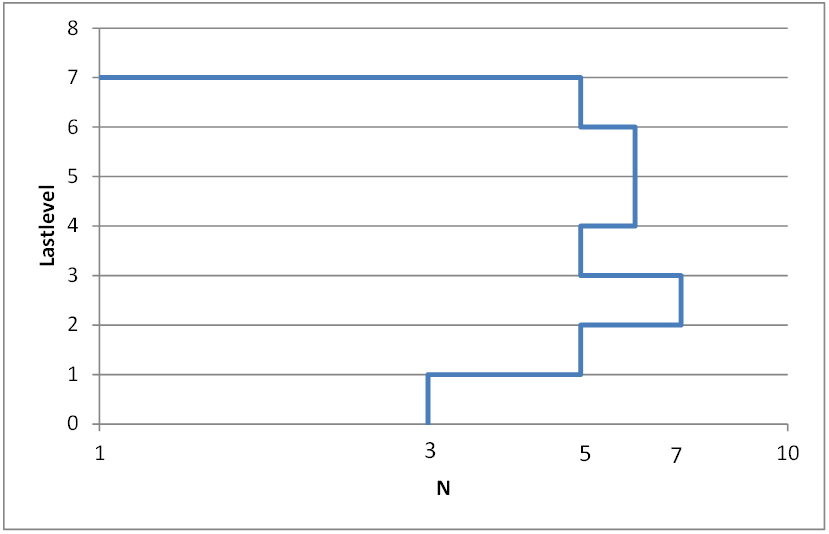
\includegraphics[width=0.3\textwidth]{gfx/level-crossing.png} 
% 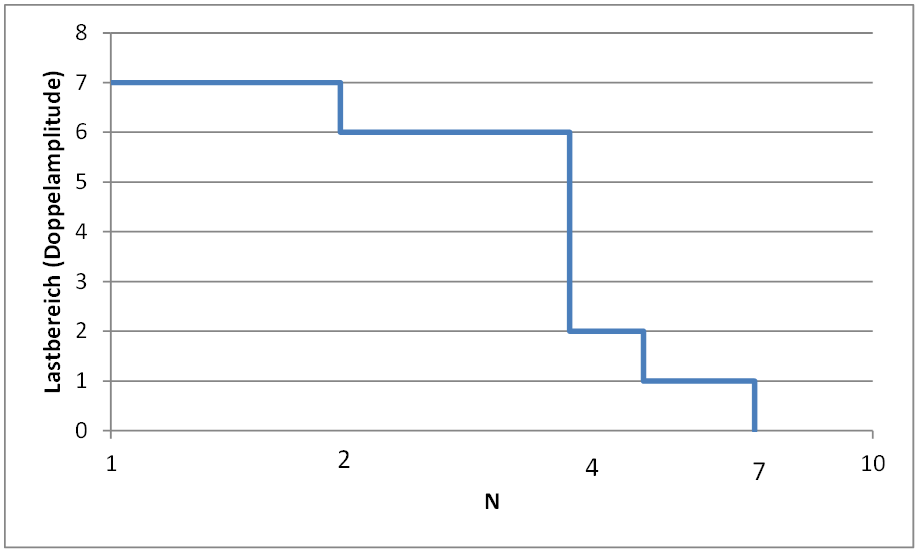
\includegraphics[width=0.3\textwidth]{gfx/range-pair.png}
% 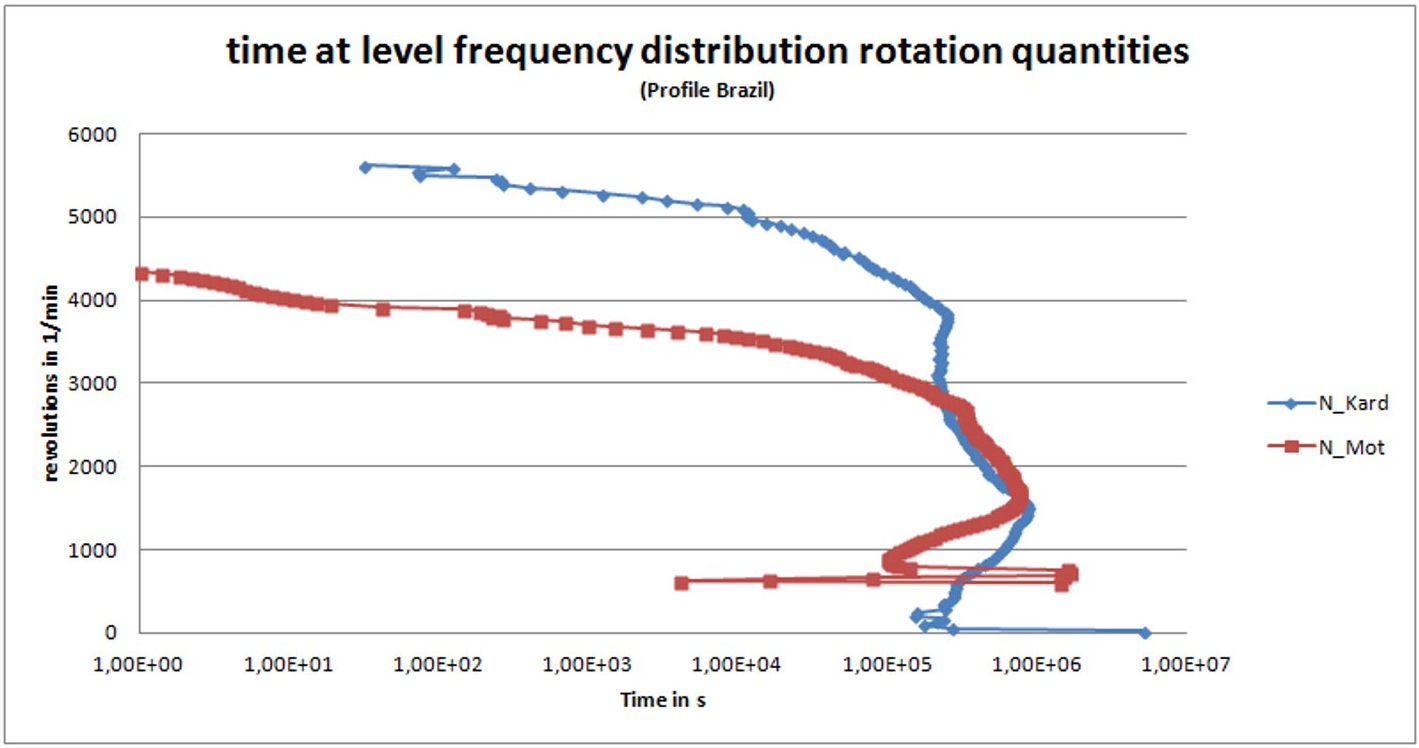
\includegraphics[width=0.3\textwidth]{gfx/time-at-level.png}
% \caption{Level Crossing, Range Pair und Time at Level vor Einsatz des Data Storytellings \cite{BenediktMundl.2023}}
% \label{fig:countingMethods}
% \end{figure}
% \noindent
% 3. Ordnung schaffen:\\
% 4. Aufmerksamkeit bündeln:\\
% 5. Geschichte erzählen:\\
\subsection{Zeitreihen}
\label{sec:timeseries}
1. Kontext verstehen: \\
Die Zeitreihen werden dazu genutzt, die Kräfte, die auf die Bauteile wirken, detailreich darzustellen. Die Kräfte werden meistens in einer Frequenz von 500\,Hz über einen festen Zeitraum gemessen. Eine Zeitreihe ist ein Werkzeug aus der Statistik, das allgemein dazu verwendet wird, Werte über den Verlauf eines Zeitraums darzustellen \cite{Billeter.1981}.
\\\\
2. Darstellung wählen:\\
Laut \cite{Gotz.2020} sind Zeitreihen ein fester Bestandteil des Bereiches der Betriebsfestigkeit. Deswegen ergibt es Sinn, nicht von der allgemeinen Darstellung abzuweichen. Zeitreihen werden ausschließlich als Linegraph dargestellt, da es sich klar um einen einzelnen Wert über eine bestimmte Zeit handelt. Es ist auf keinen Fall sinnvoll, von den bereits etablierten Graphen abzuweichen, da das den Cognitive Load für den Benutzer erhöhen würde.
\\\\
3. Ordnung schaffen:\\
\begin{figure}[h!]
\centering
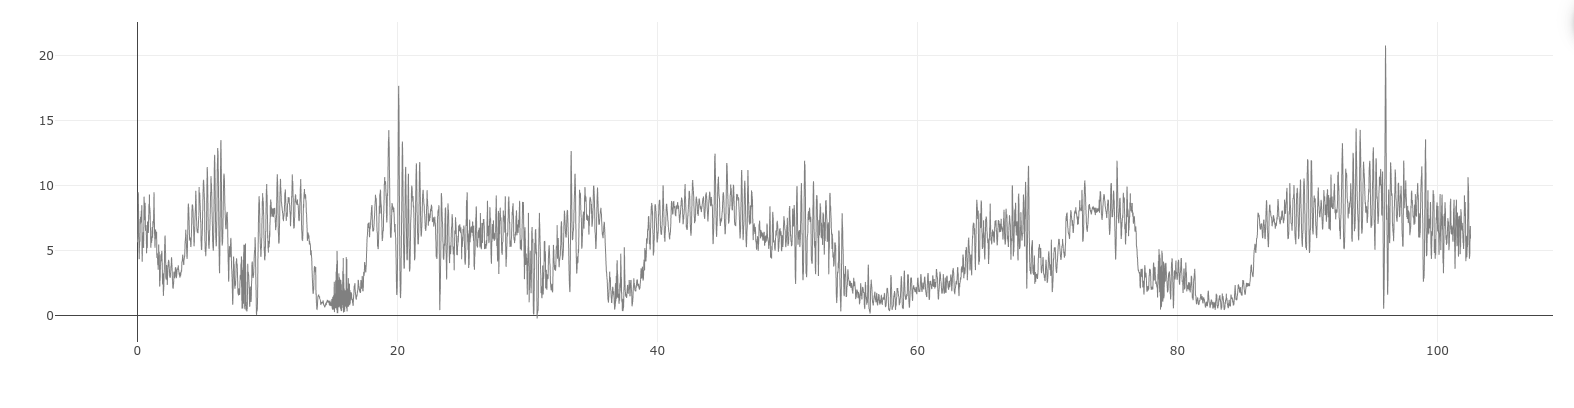
\includegraphics[width=\textwidth]{gfx/Zeitreihe_before.png} 
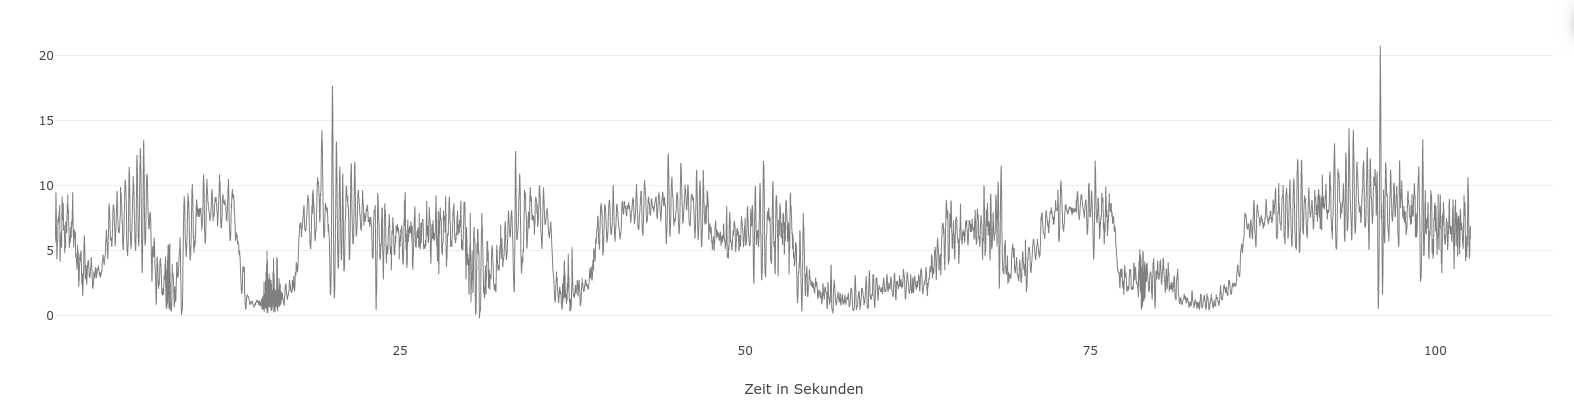
\includegraphics[width=\textwidth]{gfx/Zeitreihe_after.png}
\caption{Zeitreihe vor und nach dem Ordnungschaffen}
\label{fig:timeSeries_Before_After}
\end{figure}
\noindent
Der Defaultlinegraph von plotly.js ist in Abbildung \ref{fig:timeSeries_Before_After} zu sehen. Um Ordnung zu schaffen, wird die Nulllinie entfärbt sowie die x-Achse auf null fixiert. Es handelt sich um eine Zeitreihe, und es gibt keine negative Zeit in diesem Anwendungsfall, da die Messung immer bei null Sekunden startet. Bei der y-Achse wird die Null entfernt, da sich die beiden Nullen von der x- und y-Achse sonst überschneiden würden. Dazu werden die Ticks auf der x-Achse auf vier Stück pro Graph begrenzt, die sich automatisch berechnen. Auch die hellen Linien im Hintergrund der Ticks aus der x-Achse werden entfernt. Zudem wird bei der Hoverfunktion des Graphen für Ordnung gesorgt. Das Label hat eine dezentere Hintergrundfarbe und die Werte, die im Label dargestellt werden, werden gerundet. Diese Änderung ist in Abbildung \ref{fig:timeSeries_label_Before_After} zu sehen. 
Auch der Graph nach dem Ordnungschaffen ist in Abbildung \ref{fig:timeSeries_Before_After} zu betrachten.\\\\
\begin{figure}[h!]
\centering
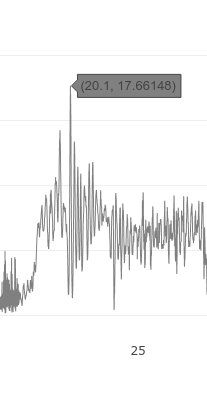
\includegraphics[width=0.15\textwidth]{gfx/Zeitreihe_label_before.png} 
\hspace*{+2cm}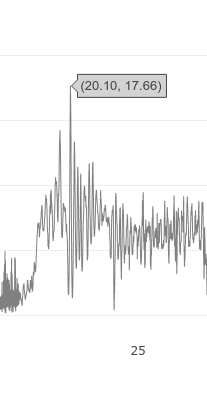
\includegraphics[width=0.15\textwidth]{gfx/Zeitreihe_label_after.png}
\caption{Hoverlabel der Zeitreihe vorher und nachher}
\label{fig:timeSeries_label_Before_After}
\end{figure}
\noindent
4. Aufmerksamkeit bündeln:\\
Bei den Zeitreihen gibt es, in Bezug auf den Punkt „Aufmerksamkeit bündeln“, einen Sonderfall, da die Trenderkennung von Anfang an genutzt werden kann. Die Minima und Maxima sind bei den Zeitreihen am interessantesten für die Benutzer, also bietet es sich an, diese direkt am Anfang anzuzeigen und die anderen Komponenten der Trenderkennung optional einbindbar zu gestalten. Durch das Markieren der Minima und Maxima wird die Aufmerksamkeit des Benutzers unmittelbar auf die wichtigen Punkte gelenkt. Zusätzlich lassen sich per Seitenmenü die anderen Trenderkennungsteile aktivieren und für den Nutzer dynamisch ändern. Bei den Minima und Maxima werden, wie bereits in der Trenderkennung, die Markerfarben und -größen geändert, damit sie herausstechen. Allerdings reicht es, für beide jeweils die gleiche Farbe zu nutzen, da durch die Ausrichtung der markierten Punkte klar wird, was ein Minimum und was ein Maximum ist. Auch bietet es sich an, die Drifterkennung direkt erkennbar zu machen, ohne dass der Benutzer diese händisch aktivieren müsste. \\\\
5. Geschichte erzählen:\\
Die Geschichte dieses Graphen wird mit der Trenderkennung erzählt. Wo sind Minima und Maxima, wo tritt ein Drift oder Offset auf, welche Werte springen über den Wertebereich -- all diese Fragen werden mit der Trenderkennung geklärt und für den Benutzer dargestellt. Wichtig ist dabei, dass die Trenderkennung dynamisch bleibt, da je nach Zeitreihe und je nach Bauteil unterschiedliche Maxima und Minima auftreten können. Dazu wird ein Seitenmenü erstellt, das die verschiedenen Teile der Trenderkennung aktivierbar sowie dynamisch einstellbar macht. Beispielhaft wird das Seitenmenü mit dynamischer Anpassung in Abbildung  \ref{fig:zeitreihe_mit_trenderkennung} dargestellt.
\begin{figure}[h!]
    \centering
    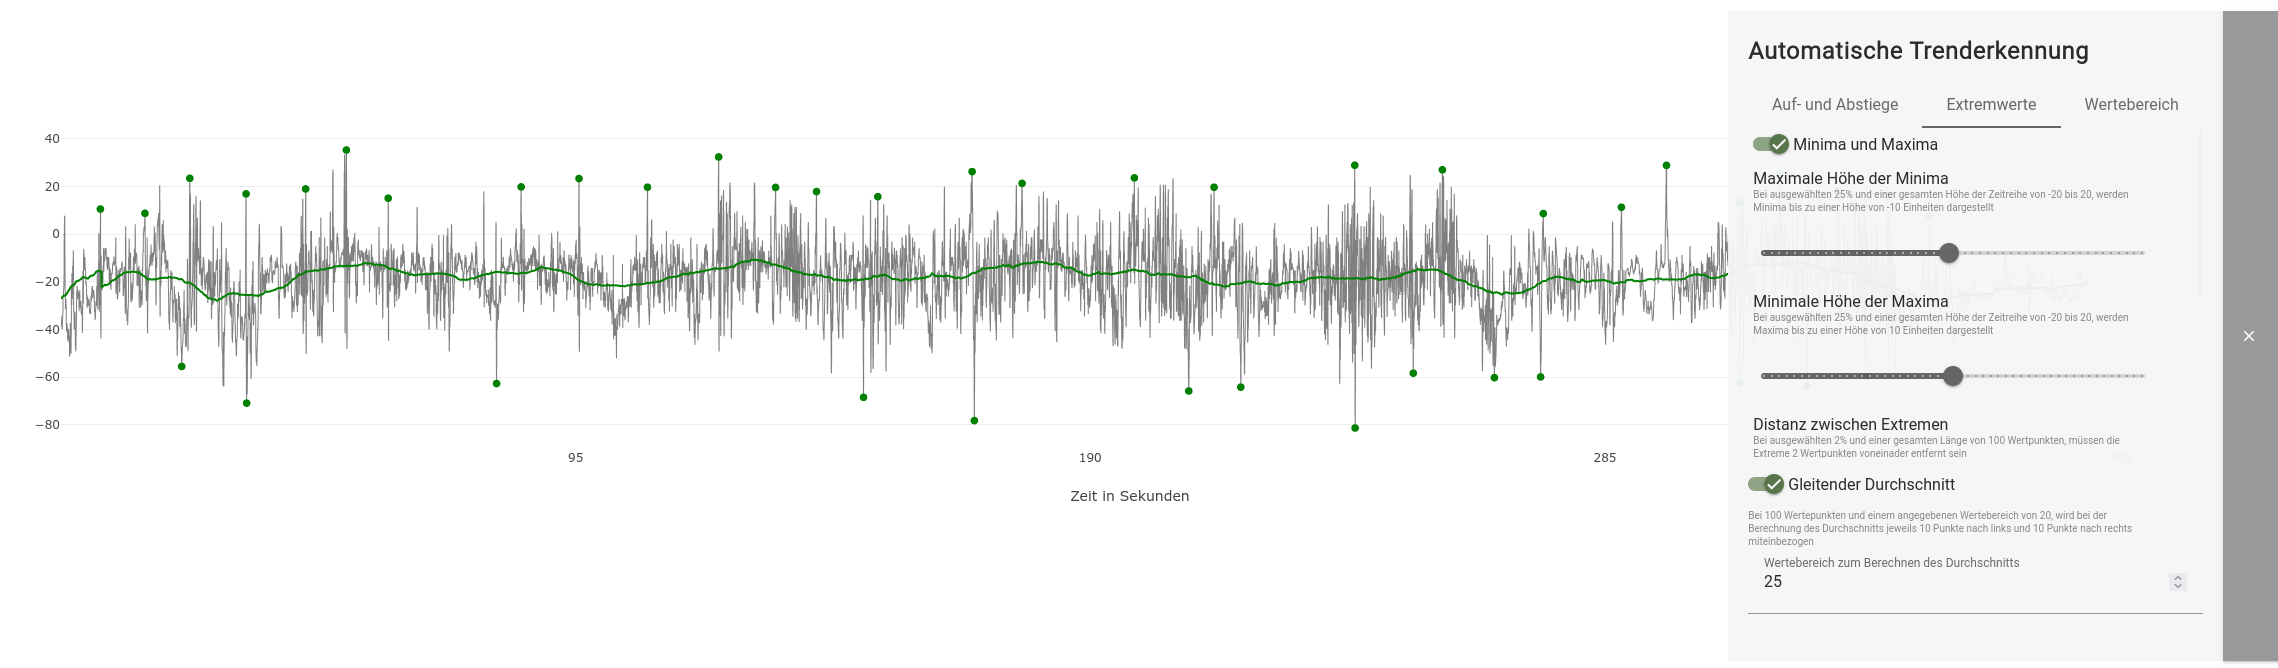
\includegraphics[width=\linewidth]{gfx/zeitreihe_mit_trenderkennung.png}
    \caption{Zeitreihe mit Trenderkennungsmenü sowie dynamisch eingestelltem gleitendem Durchschnitt}
    \label{fig:zeitreihe_mit_trenderkennung}
\end{figure}
\chapter{Implementation der Webseite}
Webseiten sind einfach zu erreichen, da für die Verwendung nur ein Browser benötigt wird. Daher fiel bei diesem Projekt die Wahl auf eine Implementation mittels Webseite. Die Webseite wird mit Angular entwickelt. Wie bereits erwähnt, gibt es bereits ein Monorepository, das auf Angular Material aufbaut. Für die Implementation von dem Monorepository wurde Nx verwendet \cite{Nx.}.  Angular Material ist eine Komponenten-Bibliothek, die verschiedene visuelle Komponenten bereitstellt, wie Buttons, Form-Fields mit verschiedenen Eingabemöglichkeiten und Slider. Da die Bibliothek von den Angular-Entwicklern selbst implementiert wurde, sind alle Komponenten bereits getestet und lassen sich ohne Probleme integrieren und erweitern \cite{Angular.2024}. Angular  basiert auf einem Komponentensystem. Das bedeutet, Angular wird aus verschiedenen Komponenten zusammengesetzt, die alle eigenes HTML, TypeScript und eigenen CSS-Code haben. Also können Komponenten beliebig oft verwendet werden und sind in ihrer Funktionalität trotzdem geschlossen. In dem bestehenden Monorepository gibt es verschiedene geteilte Komponenten, beispielsweise einen App-Core, der für alle Apps die Navigation und das Routing implementiert, Fehlerbehandlung, Authentifizierung und verschiedene visuelle Komponenten, die auch in dieser Webseite verwendet werden. Zu den visuellen Komponenten zählen:
\begin{multicols}{3}
    \begin{itemize}
        \item Buttons
        \item Cards
        \item Charts 
        \item Dynamic Dialog
        \item Loading Indicator
        \item Table
        \item Map
        \item Warning
        \item Error Stacker
    \end{itemize}
\end{multicols}
\noindent
Die geteilten Komponenten nutzen, genau wie die Angular-Material-Komponenten, Farbpaletten, die jeweils eine primäre, eine Akzent-, eine Warn- und eine Success-Farbe zugewiesen bekommen. Auf der Primärfarbe basieren die verschiedenen grünen Farbtöne, die in den Data-Storytelling-Graphen verwendet wurden. Dazu wurde das Tool coolors \cite{FabrizioBianchi.} genutzt, um jeweils hellere und dunklere Töne basierend auf der Farbe zu erzeugen.
\begin{figure}[h!]
\centering
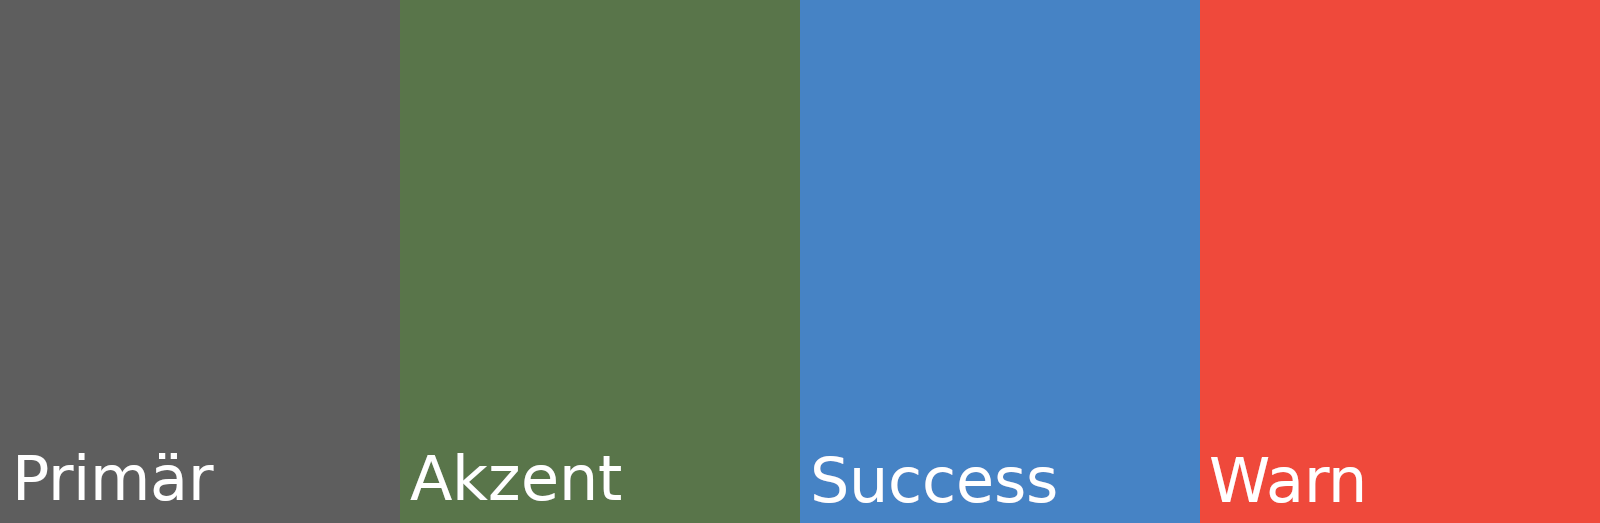
\includegraphics[scale=0.6]{gfx/palette.png}
\caption{Farbpalette für die Webseite}
\label{fig:palette}
\end{figure}
\\\\Die App-Core-Komponente, die die Webseite auch nutzt, generiert die Navigation für die App automatisch aus einer JSON-Datei und transformiert die Navigation, je nachdem welche Unterseite aufgerufen ist. Die Navigation, die in der JSON-Datei festgelegt wird, entspricht dem Datentyp \texttt{NavigationItem} aus \ref{appendix:dataset_types}. Über die Komponente wird auch das Ein- und Ausloggen durchgeführt. Für das User-Management wird Keycloak verwendet \cite{KeycloakAuthorsTheLinuxFoundation.2023}. Die Navigationskomponente übernimmt auch das Routing für die Unterseiten. Diese werden als einfache Bibliotheken mit eigenen Komponenten und Services angelegt. Zusätzlich gibt es einen automatischen Ladebalken, der jedes Mal, wenn eine Aktion mit dem Netzwerk ausgeführt wird, eingeblendet wird. Der Ladebalken kann anhand von einem Tutorial implementiert werden \cite{KeithStrickland.2020} und die Navigation ist ähnlich einem vorhandenen Beispiel \cite{sahilshah.2023}.
\\\\ 
Allgemein gibt es für Angular gute Tutorials, bei der Entwicklung der Webseite wurde unter anderem auf die Anleitungen von \cite{Angular.2022} für die allgemeine Implementation, \cite{DavidAkim.2022} für die Benutzung von plotly.js mit Angular und \cite{JonathanCardoso.2021} für die Verwendung von generics in Typescript zurückgegriffen.
\section{Implementation API und State}
Die Implementation der API wurde durch die bereits existierende Monorepository-Struktur und durch die Verwendung von @NgRx/data \cite{NgRx.io.2024} deutlich vereinfacht. Ohne diese Erweiterung muss für jede Schnittstelle ein Service angelegt werden, der die Anfragen steuert. Mit @NgRx/data und einem generischen Services wird diese Arbeit zumindest für die CRUD-Anfragen (Create, Read, Update und Delete) abgenommen. Die Erstellung eines generischen Datenservice zum Abwickeln der CRUD-Anfragen wird in folgendem Tutorial beschrieben: \cite{A.Waris.2023}.
Dieser generische Datenservice vererbt mithilfe von dem Keyword \texttt{extends} an die einzelnen Entitätenservices, die von @NgRx/data erstellt wurden, und somit können die bereits vorhandenen CRUD-Funktionen in Sonderfällen pro Entität angepasst werden \cite{MicrosoftTypeScript.2024}.  
Zudem wurde bei der Erstellung des Monorepositorys darauf geachtet, die Datentypen möglichst wiederzuverwenden, deshalb können viele Services genutzt werden, die bereits existieren.\\
Eine Besonderheit von NgRx ist die Bereitstellung einer Funktionalität mit Namen Store, dabei wird lokales State-Management für Angular-Apps bereitgestellt \cite{NgRx.io.2024b}. Es wird nicht nur für jede Unterseite ein eigener State erstellt, der Informationen Unterseiten übergreifend bereitstellen kann, sondern auch der Zugriff auf die Daten erleichtert, die von den API-Anfragen zurückgegeben werden. Dadurch kann es Usern ermöglicht werden, auch nach dem Navigieren auf der Seite wieder zu ihren ausgewählten Analysen zurückzukommen. NgRx benutzt verschiedene Komponenten, um das State-Management zu ermöglichen. In der folgenden Abbildung \ref{fig:NgRx} von \cite{NgRx.io.2024b} werden die verschiedenen Komponenten sowie ihr Zusammenspiel dargestellt.
\begin{figure}[!h]
    \centering
    \includegraphics[width=0.75\linewidth]{gfx/NgRx.png}
    \caption{NgRx-Flow und -Komponenten \cite{NgRx.io.2024b}}
    \label{fig:NgRx}
\end{figure}
Die Komponenten sind:
\begin{description}
    \item[selector]\hfill \\
    Die Selektoren sind dazu da, die Daten im Store für die Benutzung in den Angular-Komponenten bereitzustellen. Dabei können die Daten umgeformt oder gefiltert werden.
    \item[component]\hfill \\
    Die Angular-Komponente, die für die Darstellung der gelieferten Daten zuständig ist. Durch Benutzereingaben können Actions getriggert werden.
    \item[action]\hfill \\
    Actions sind dazu da, entweder Daten von den Benutzereingaben in den Store zu schreiben oder Effekte zu triggern. 
    \item[effects]\hfill \\
    Effekte sind für die Kommunikation mit den von @NgRx/data erstellten Services vorgesehen. Sie starten die API-Anfragen und können die Ergebnisse verwalten. Außerdem können die Effekte erneut Actions abschicken, um beispielsweise Fehlermeldungen oder Anfragen, die von anderen Anfragen abhängen, zu starten.
    \item[service]\hfill \\
    Die Services werden mit @NgRx/data erstellt und können beliebig für weitere Anfragen außerhalb von CRUD erweitert werden.
    \item[reducer]\hfill \\
    Reducer ermöglichen den Zugriff auf den Store, sowohl um die Variablen zu ändern als auch um diese zu lesen. 
    \item[store]\hfill \\
    Die bereits angefragten Daten werden hier zwischengespeichert und für jeden Selector in der App abrufbar gemacht.
\end{description}
In dem genutzten Monorepository wurde ein generischer State erstellt, der mithilfe von allgemeinen Reducern und Actions einiges an Schreibarbeit erspart. Es müssen pro Unterseite Selektoren und Effects angelegt werden. Die allgemeinen Actions basieren auf einem \texttt{ACTION\_TYPE} enum, der beispielsweise für die Selektion der zu analysierenden Daten zuständig ist. Dabei werden der \texttt{ACTION\_TYPE} für die passende Auswahl sowie die ausgewählten IDs an den State weitergegeben. Einige Beispiele, wie der \texttt{ACTION\_TYPE} enum formuliert werden kann, befinden sich in \ref{appendix:dataset_types}. 
\section{Implementation Seiten}
Im Laufe der Entwicklung wurden zusätzlich zu den bereits bekannten Seiten aus den Interviews noch weitere Seiten festgelegt. Somit werden für die Webseite die folgenden Unterseiten erstellt:
\begin{itemize}
    \item Datenbasis
    \item Alternativer Kilometerzähler
    \item Fingerprints
    \item Überwachung Dauerlauferprobung
    \item Vergleich von Einsatzdaten
\end{itemize}
Die Datenbasis wird mithilfe eines Generic Service implementiert, der übergreifend über das Monorepository alle Datenbasen erstellt. Allerdings wird in diesem Anwendungsfall das Diagramm aus \ref{section:Prozentuale_Schädigung} hinzugefügt. Dabei werden der State oder auch die API-Aufrufe von einem Base-Service geregelt. Dadurch müssen nur die geteilten Komponenten für die Datenbasis im HTML eingebunden werden. Dazu  zählen eine Komponente für die Karte, die die Einsatzorte darstellt, das hervorgehobene Rechteck neben der Karte, das die zusätzlichen Informationen zu den ausgewählten Daten zeigt, und die einzelnen Karten pro Fahrzeug. Über dieses Template wird der Graph hinzugefügt, der für jedes Fahrzeug die passenden Daten darstellt. Dazu hat die Datenbasis das Attribut „selected Vehicle“, um die passenden Daten sowohl für die zusätzlichen Informationen als auch für den Graphen zu filtern.\\\\ Der alternative Kilometerzähler wurde aufgrund der Entwicklung des Diagrammes aus \ref{section:Prozentuale_Schädigung} hinzugefügt, da es praktisch ist, alle Fahrzeuge und deren aktuelle Schädigungen auf einen Blick zu sehen. Durch einen generischen Datenservice, der die API-Aufrufe für alle Fahrzeuge regelt, lassen sich die vorhandenen Fahrzeuge über den State abfragen und in eine eigene Komponente geben, die die Darstellung pro Fahrzeug regelt. Hierfür wird der gleiche Service verwendet, der auch in der Datenbasis die Graphen bereitstellt.\\\\ Die Fingerprints sind zur alleinigen Darstellung des Diagramms für die Fingerprints da. Da es sich bei den Fingerprints um eines der wichtigsten Werkzeuge für diesen Anwendungsfall handelt, wurde die Unterseite hinzugefügt. Der State wird vom generisch implementierten State geregelt. Dabei müssen nur die Selektoren und Effekte hinzugefügt werden, die Actions und der Reducer sind für jede Seite gleich, die mit dem generischen State erstellt wurde. Da für die Seite nur die Fingerprints in der aktuellen Auswahl relevant sind und die Auswahl vom generischen State geregelt wird, wird lediglich ein Effekt mit der Anfrage an das Backend bezüglich der ausgewählten Fingerprints benötigt.\\\\
Die Dauerlauferprobung setzt sich aus den Diagrammen der Dauerlauferprobung (\ref{section:dauerlauferprobung}), des Fahrzeugbildes mit den eingefärbten Teilen (\ref{sec:vehicle-images)} und einer Tabelle mit weiteren Informationen zur Erprobung zusammen. Danach kann der Benutzer über den Graphen der Erprobung einen Punkt in der Erprobung auswählen. Über diese Auswahl wird der Graph mit der kumulierten Schädigung (\ref{section:schaedigung}) befüllt. Über diesen Graphen kann wiederum eine einzelne Messung ausgewählt werden, die dann als Zeitreihe \ref{sec:timeseries} angezeigt werden kann. Dadurch können alle relevanten Daten für die Dauerlauferprobung angezeigt werden. Alternativ kann je nach den Bedürfnissen auch nur ein grober Überblick über die vorhandenen Messungen erfasst werden. Auch der State auf dieser Seite wird vom generischen State geregelt. Durch die vielen verschiedenen Daten, die angefragt oder angezeigt werden können, werden mehrere \texttt{ACTION\_TYPES} für jede einzelne Benutzerinteraktion benötigt.\\\\
Die Seite zum Vergleich der Einsatzdaten stellt mehrere Daten gleichzeitig dar. Zunächst werden der Graph mit den Fahrzeugbildern und die gleiche Tabelle wie in der Dauerlauferprobung dargestellt. Um einen Vergleich über die Daten zu gewährleisten, wird der Graph mit der kumulierten Schädigung (\ref{section:schaedigung}) genutzt. Über die Auswahl des Benutzers können die einzelnen Messungen als Zeitreihen (\ref{sec:timeseries}) dargestellt werden. Zudem gibt es eine Darstellung, die die einzelnen Kollektive zeigt. Sie wurde in dieser Arbeit nicht mit Data-Storytelling überarbeitet, da Kollektive eine feste Größe im Feld der Betriebsfestigkeit \cite{Gotz.2020} sind. Bei den Kollektiven werden laut \cite{PatrickPfeiffer.17.10.2022} lediglich die höchsten Ausschläge des Messsignals betrachtet. Da es bei der Darstellung der Kollektive nicht möglich ist, einen Handlungsaufruf zu starten oder sonstige Points of Interest hervorzuheben, eignet sich diese Darstellungsart nicht für das Data-Storytelling. Der State der Vergleich von Einsatzdatenseite wird vom generischen State abgewickelt. Die API für die Fingerprints und die Dauerlauferprobung sind vor Fertigstellung dieser Masterarbeit noch nicht fertig implementiert, weswegen auf der Webseite aktuell für beide ein Beispieldatensatz im passenden Format bereitgestellt wird.\\\\
Alle Unterseiten sind gleich aufgebaut. Zuerst wird eine Containerkomponente implementiert, die die Verteilung der Daten an die Unterkomponenten regelt. Im HTML dieser Komponente wird der Seitenaufbau erstellt und es werden die Unterkomponenten angesprochen. Die einzelnen Unterkomponenten sprechen die passenden Services an, um die Visualisierungen zu erstellen. Die Daten, die in den Services weiterverarbeitet werden, werden an verschiedene Komponenten weitergeleitet, um die Daten darzustellen, beispielsweise die Shared-Chart- oder die Shared-Tabellen-Komponenten. Da sich auf den Seiten einige Diagramme und Visualisierungen wiederholen, bietet es sich an, diese in eigene Komponenten auszulagern, beispielsweise die Fingerprints oder die Fahrzeugvisualisierung mit den Bildern und Image-Maps. Dadurch lässt sich vermeiden, dass sich Codestücke wiederholen. Auch die Komponente zur Auswahl der Fahrzeuge wird einmal implementiert und dann mithilfe des Komponentensystems auf mehreren Seiten genutzt. Die Auswahl hat einen Toggle, über den entschieden werden kann, ob die Auswahl für Einzelfahrzeuge oder für Fahrzeugtypen gelten soll. Anhand dieser Auswahl wird eine JSON-Konfiguration erstellt und die Auswahl dynamisch erzeugt. Die JSON-Konfiguration wird mittels des Datentyps \texttt{DynamicDataSelectData} in \ref{appendix:dataset_types} erstellt. Dadurch können beliebig viele Auswahlfelder, eine Warnung oder ein Button konfiguriert werden. Jedes Auswahlfeld wird mit dem Typ \texttt{DynamicDataSelectControls} erstellt. Dabei ist insbesondere das Feld \texttt{influences} interessant, da dadurch Beziehungen zwischen den Feldern ausgewiesen werden können. Für zusätzliche Validierungen können die Typen \texttt{DynamicFormValidatorConfig} oder \texttt{DynamicFormAdditionalConfig} genutzt werden, beispielsweise kann hier auch die Optionalität der Felder konfiguriert werden.
\section{Implementation Graphen}
Die Graphen werden mit plotly.js für Angular implementiert. Grundsätzlich setzen sich die Charts aus Layout und Traces zusammen, in \ref{appendix:graph_types} ist das passende Interface \texttt{Chart} zu sehen. Das Layout ist für die visuelle Darstellung des gesamten Graphen verantwortlich, während die Traces die einzelnen Wertedarstellungen bilden. Generell gibt es bei plotly.js mehrere Wege, um Informationen zusätzlich zu den x- und y-Werten anzuzeigen. Laut der plotly.js-Dokumentation \cite{Plotly.2024b} gibt es sowohl Annotations als auch Shapes, um die Graphen zu erweitern.\\\\ Bei der Erstellung der Graphen wird pro Graph ein Service erstellt, der die Daten auswertet und wenn nötig transformiert sowie das Layout bildet und an die Chart-Komponente weitergibt. Um beispielsweise den Zeitreihen-Graphen darzustellen, wird ein Layout mit den folgenden Parametern erstellt:
\begin{lstlisting}[language=Typescript]
    {
      showlegend: false,
      annotations: this.createAnnotations(testData.values, trends),
      shapes: this.createShapesForRisesAndFalls(time, trends),
      hoverlabel: { bgcolor: 'lightgray' },
      xaxis: {
        zeroline: false,
        rangemode: 'tozero',
        autorange: true,
        tickvals: tickvals.map((val) => val * tickSteps),
        ticktext: [''].concat(
          tickvals.slice(1).map((val) => (val * tickSteps).toString())
        ),
        title: { text: 'Zeit in Sekunden' },
        showgrid: false,
        hoverformat: '.2f',
      },
      yaxis: {
        zeroline: false,
        autorange: true,
        hoverformat: '.2f',
      },
    };
\end{lstlisting}
Die Annotations und Shapes werden von einer separaten Funktion mit den nötigen Werten für die Trenderkennung gefüllt. Der Parameter \texttt{showlegend} konfiguriert, ob die Legende dargestellt werden soll, in der die verschiedenen Traces angezeigt werden. Durch den Parameter \texttt{hoverlabel} kann das Hoverlabel mit verschiedenen Variablen angepasst werden, wie in diesem Beispiel der Hintergrundfarbe. Andere Anpassungsmöglichkeiten sind die Farbe, Schriftart, ob noch zusätzliche Informationen im Hoverlabel angezeigt werden sollen und verschiedene Formatierungsmöglichkeiten für diese Informationen. Es lassen sich sowohl die x- als auch die y-Achse genau anpassen. Bei dem Layout für die Zeitreihen ist besonders interessant, dass durch die Überschneidung des Nullpunktes auf beiden Achsen zweimal die Null angezeigt wurde. Aufgrund der Reduzierung des Visual Clutters beim Data-Storytelling wird durch die Funktion, die im Layout in der x-Achse die \texttt{tickvals} und den \texttt{ticktext} berechnet, die Null auf der x-Achse durch einen leeren String ersetzt. Das reduziert die Darstellung um eine Null für den Punkt an den sich die beiden Achsen schneiden, anstatt zwei Nullen nebeneinander darzustellen. Die \texttt{tickvals} legen fest, wo auf der Achse ein Tick gesetzt werden soll. Dieser Wert wird durch eine einfache Berechnung ermittelt, die die Dauer der Zeitreihe durch vier teilt und das Ergebnis dann rundet, um auf eine sinnvolle Zahl zu kommen. Dadurch werden immer vier Ticks dargestellt. Die Parameter \texttt{zeroline} und \texttt{showgrid} sind beide für die Darstellung des Grids zuständig, wobei \texttt{zeroline} die Nulllinie hervorhebt und \texttt{showgrid} das Grid vollständig ausblendet. Das Attribut \texttt{rangemode} gibt an, welcher Art die Beschränkungen des Grids sind: Bei \texttt{tozero} ist die Nulllinie die untere Grenze des Grids, bei \texttt{auto} wird das Grid passend zu den Graphen skaliert. Das \texttt{hoverformat} schränkt die Formatierung im Hoverlabel auf zwei Stellen hinter dem Komma ein.\\ Für die Erstellung der Wertedarstellungen wird ebenfalls ein Objekt definiert. Dieses ist im Folgenden am Beispiel der Zeitreihen abgebildet:
\begin{lstlisting}[language=Typescript]
    {
        x: this.calculateTimeForFrequency(
          testData.frequency,
          testData.values.length
        ),
        y: testData.values,
        hoverinfo: 'name +x+y',
        type: 'scattergl',
        mode: 'lines+markers',
        marker: {
          color: this.getColorForMarkers(
            trends?.maximaAndMinima,
            testData.values
          ),
          size: 8,
        },
        line: {
          color: 'gray',
          width: 1,
        },
        name: 'Zeitreihe',
    },
\end{lstlisting}
Es werden zunächst zwei Arrays mit den jeweiligen x- und y-Werten festgelegt. Anschließend folgt die Zusammensetzung der Daten, die im Hoverlabel dargestellt werden. Als \texttt{type} wird der Typ der Wertedarstellung definiert, der Default-Wert ist meist \texttt{scatter}. Weil aber besonders bei der Trenderkennung die Implementation der Darstellungen und Rechnungen aufwendiger war, was zu Performanceeinbußen führte, wenn der Graph als klassisches SVG implementiert wurde, wurde der Typ \texttt{scattergl} gewählt. Dadurch hat plotly.js die Möglichkeit, die Graphen auch mit WebGL rendern zu lassen. WebGL ist laut \cite{MDNcontributors.2024b} eine JavaScript-API, die mithilfe von OpenGL in der Lage ist, die Hardware des Computers durch den Browser anzusteuern, und dadurch die Zeit für das Rendern des Graphen deutlich minimieren kann \cite{Plotly.2024b}. Durch den \texttt{mode} lässt sich die Darstellung der Werte als Linien, Marker oder beides anwenden. Zuletzt können die Marker und die Linien jeweils mit Farben und Größen visuell angepasst werden. Mit dem Parameter \texttt{name} wird der Name festgelegt, der beispielsweise in der Legende verwendet wird. 
Durch diese Vorgehensweise können mit plotly.js alle in dieser Arbeit erstellten Graphen implementiert werden.

\chapter{Evaluation}
% die MinMax und Schädigungswerte sind doch nicht kumuliert ?
\section{Vergleich zwischen alter und neuer Webseite}
Insgesamt haben sich die Graphen der alten Webseite durch den Einsatz von Data-Storytelling deutlich verändert. Bereits im Laufe der Arbeit wurden einige Beispiele der alten Graphen ohne Data-Storytelling gezeigt. Dabei hat sich besonders der Graph zur Darstellung der kumulierten Schädigung aller gemessenen Durchfahrten verändert. Die Schwierigkeit bei diesem Graphen ist die Menge an Daten, die dargestellt werden soll. Dadurch ist es besonders auf der alten Webseite schwierig, auf einen Blick zu erkennen, welche Daten  relevant sind. Durch den Einsatz des Data-Storytellings konnten die Reize, die auf den Benutzer wirken, reduziert und die wichtigen Punkte des Graphen hervorgehoben werden. In der folgenden direkten Gegenüberstellung in Abbildung \ref{fig:schädigung_vergleich} ist die Verbesserung, trotz verschiedener Daten, gut zu erkennen.\\
\begin{figure}[!h]
    \centering
    \includegraphics[width=1\linewidth]{gfx/schädigung_davor.png}
    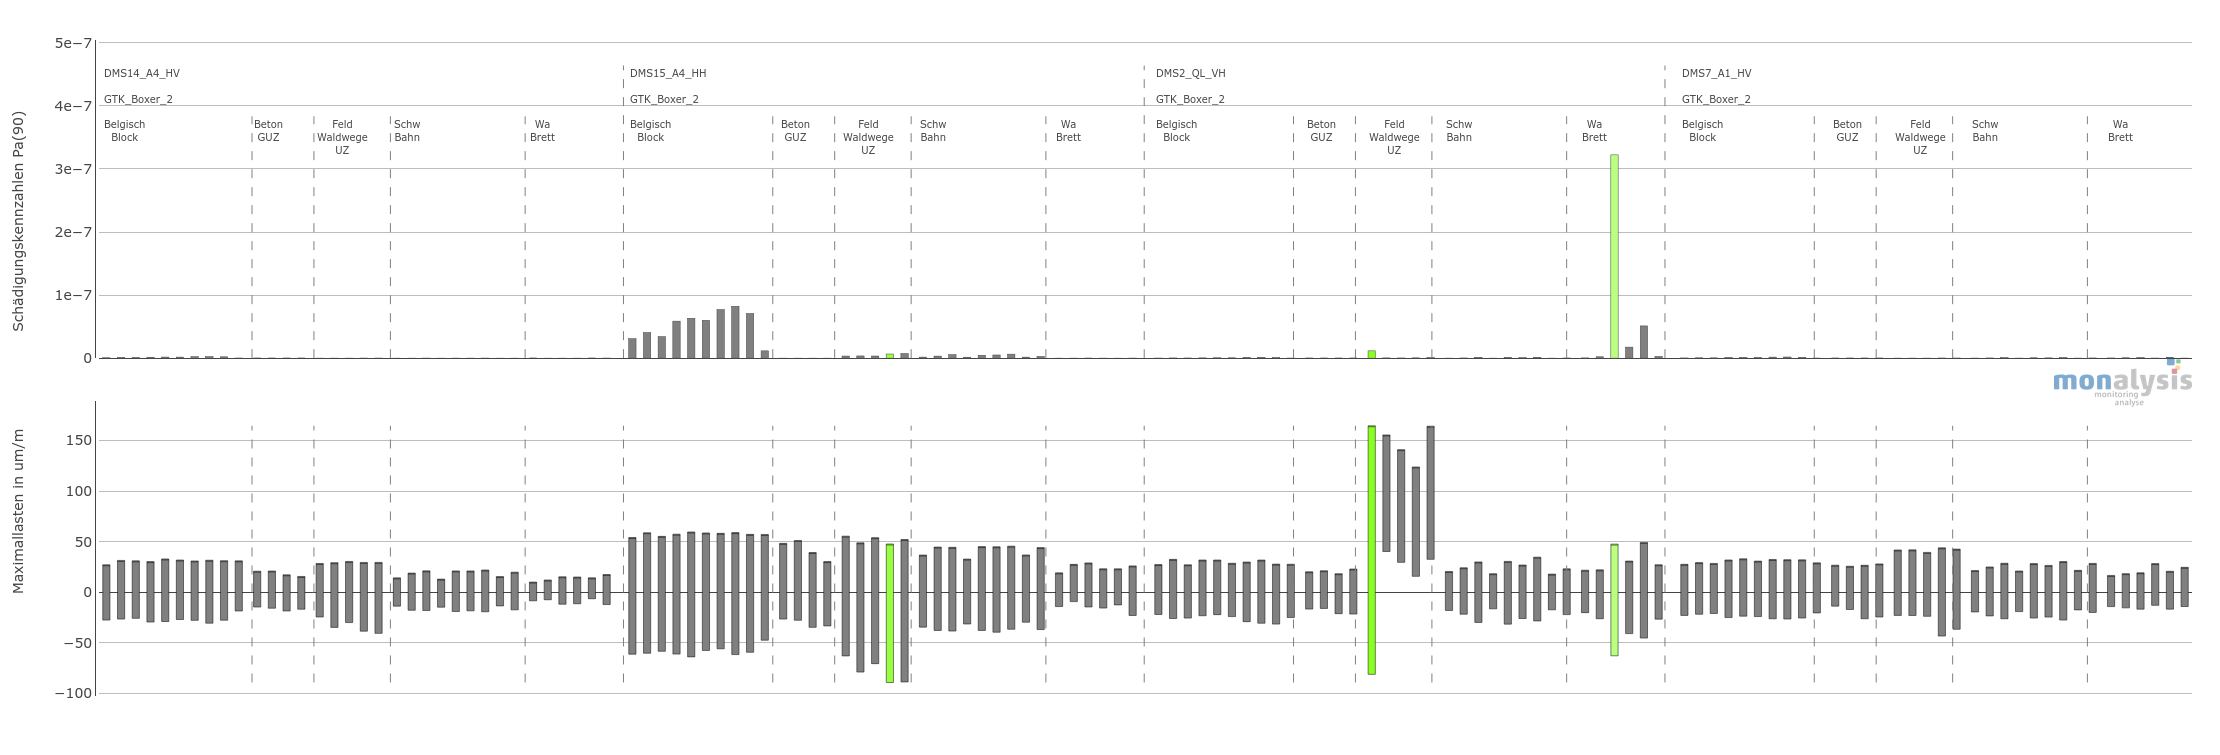
\includegraphics[width=1\linewidth]{gfx/new_schaedigung.png}
    \caption{Graph mit der kumulierten Schädigung im Vergleich}
    \label{fig:schädigung_vergleich}
\end{figure}
\noindent
Insbesondere bei Aktivierung des Top-Filters kann durch das Data-Storytelling schneller erkannt werden, welche Daten wie beschaffen sind \ref{fig:top_filter_vergleich}. 
\begin{figure}
    \centering
    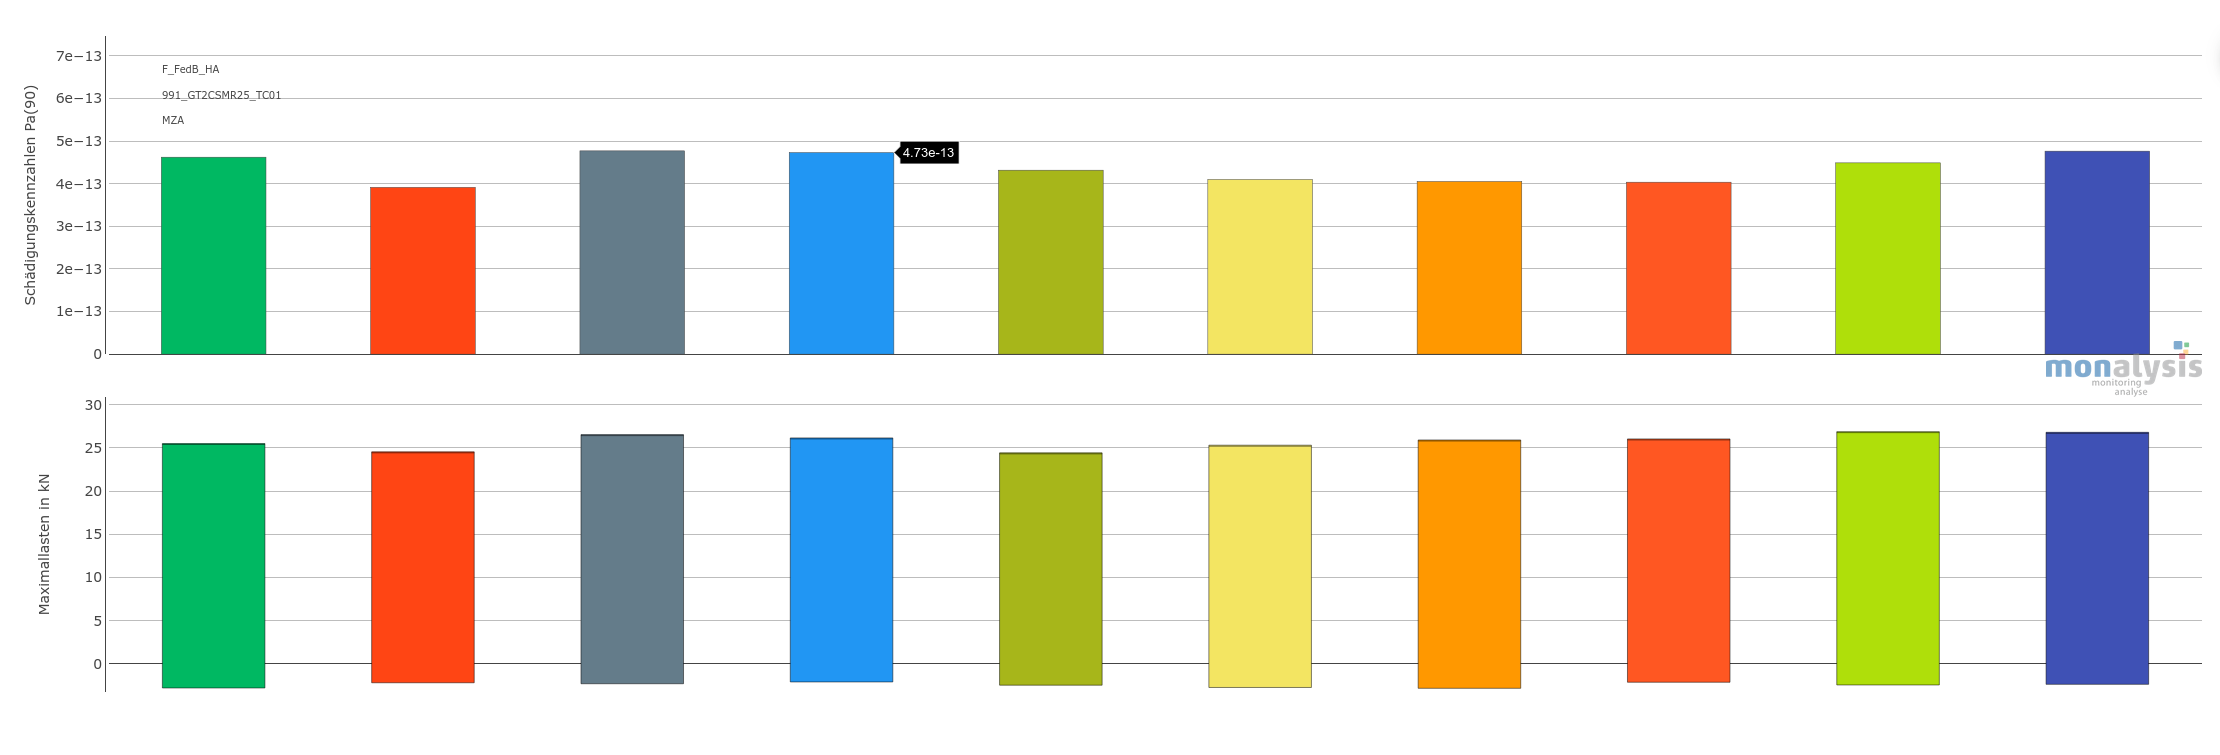
\includegraphics[width=1\linewidth]{gfx/top_vergleich_alt.png}
    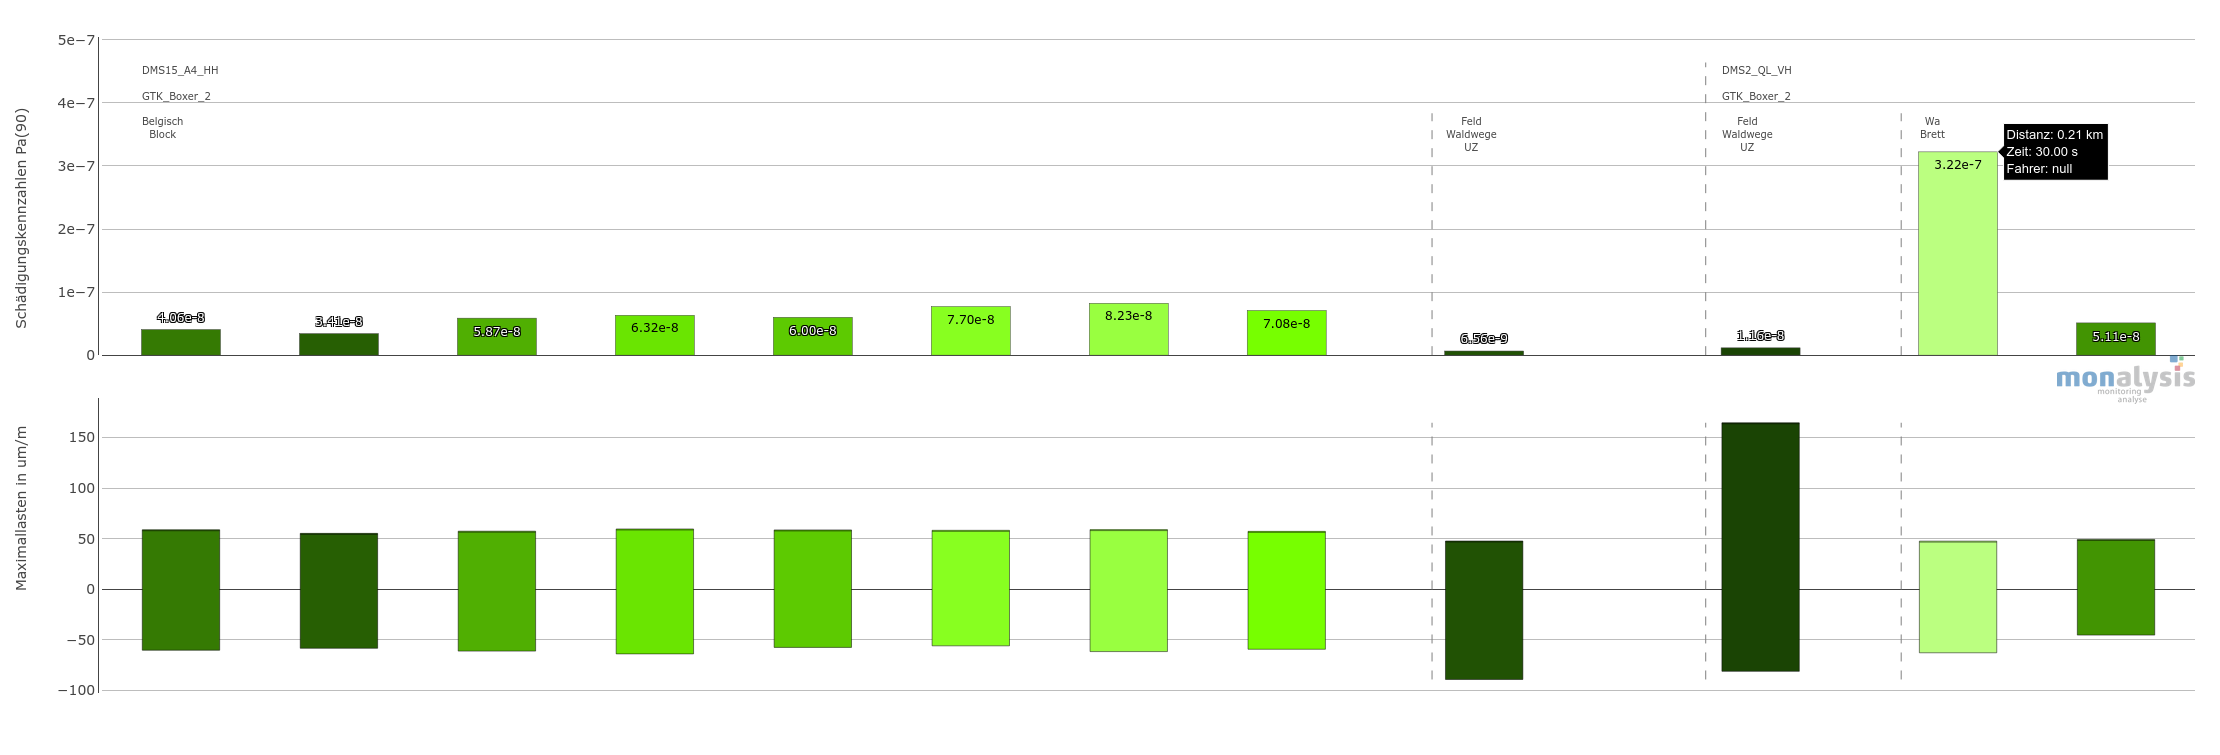
\includegraphics[width=1\linewidth]{gfx/top_vergleich_neu.png}
    \caption{Graph mit der kumulierten Schädigung im Vergleich mit Top-Filter}
    \label{fig:top_filter_vergleich}
\end{figure}
\noindent
Ein weiterer Graph, der ebenfalls bereits ohne Data-Storytelling existiert, sind die Zeitreihen. Diese werden in der alten Webseite nur als Linegraph dargestellt und wurden in dieser Arbeit durch die Trenderkennung erweitert. Dadurch können bei der Benutzung der Trenderkennung viele Erkenntnisse schnell und visuell ansprechend gewonnen werden. Werden die Graphen als Bilder exportiert, wird die Trenderkennung ebenfalls auf den exportierten Bildern dargestellt. In Abbildung \ref{fig:timeseries_compare} sind die beiden Zeitreihen-Darstellungen im direkten Vergleich zu sehen.\\
% der vergleich ist hier eigentlich nur sinnvoll, wenn du 2x die gleiche zeitreihe nimmst +  kleinerer ausschnitt, sonst sieht man am bildschirm die eingezeichneten grenzen, extremwerte etc kaum
\begin{figure}[!h]
    \centering
    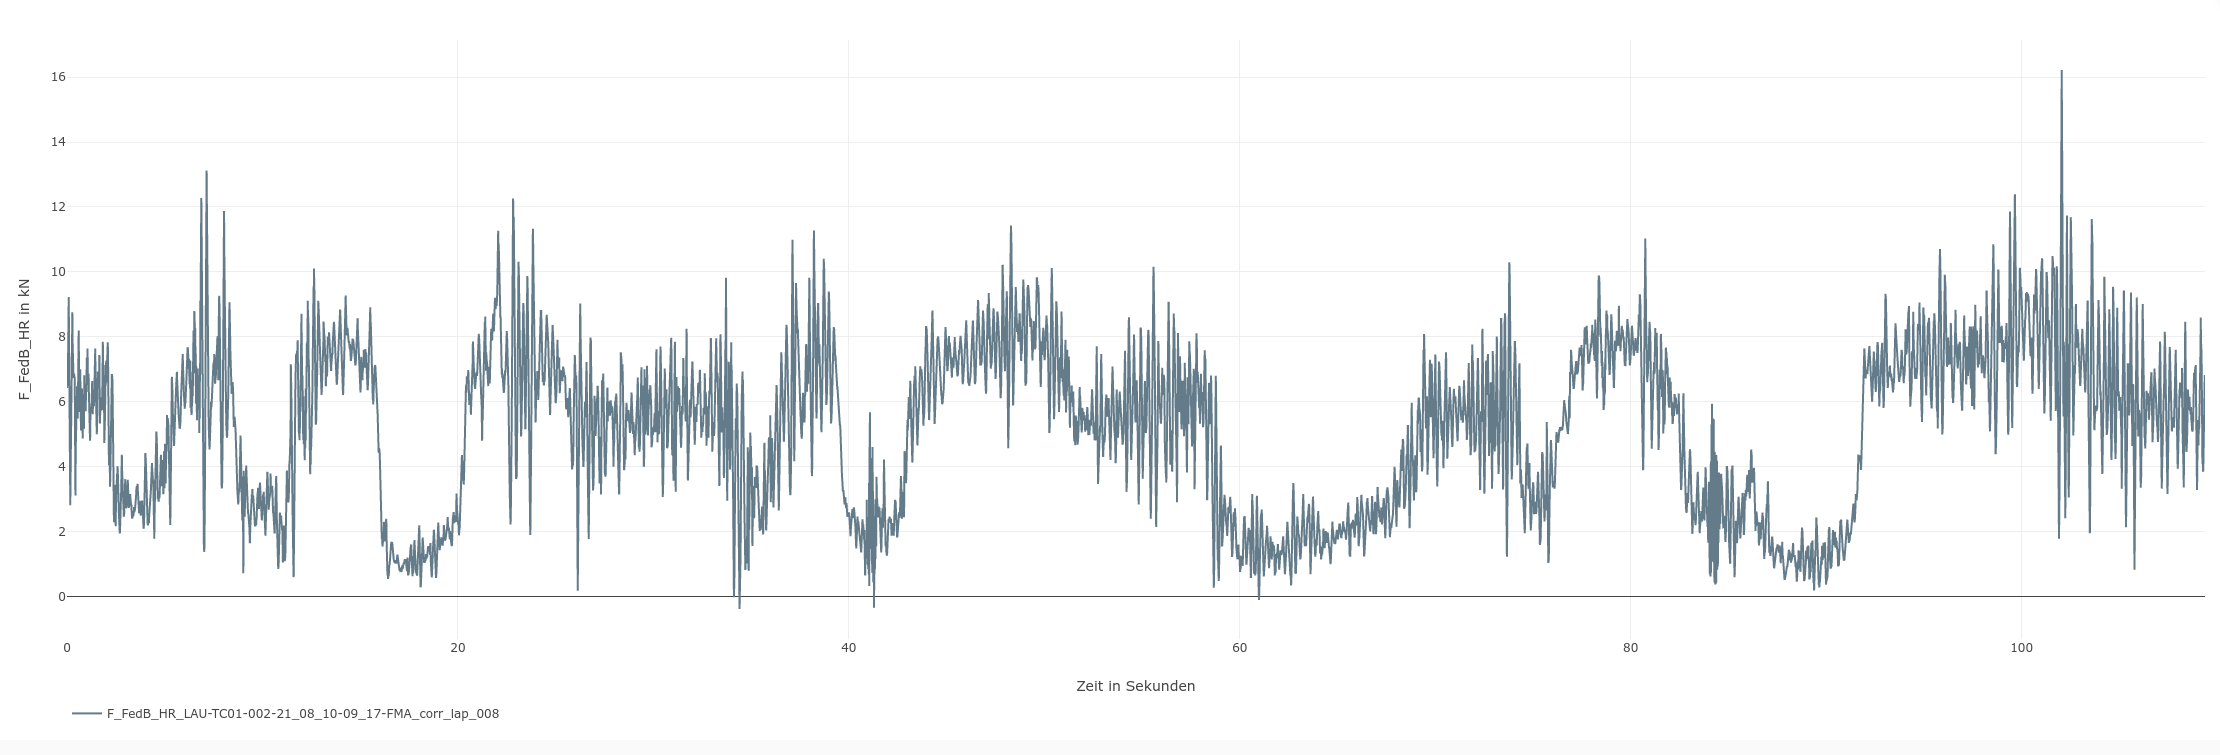
\includegraphics[width=1\linewidth]{gfx/timeseries_old.png}
    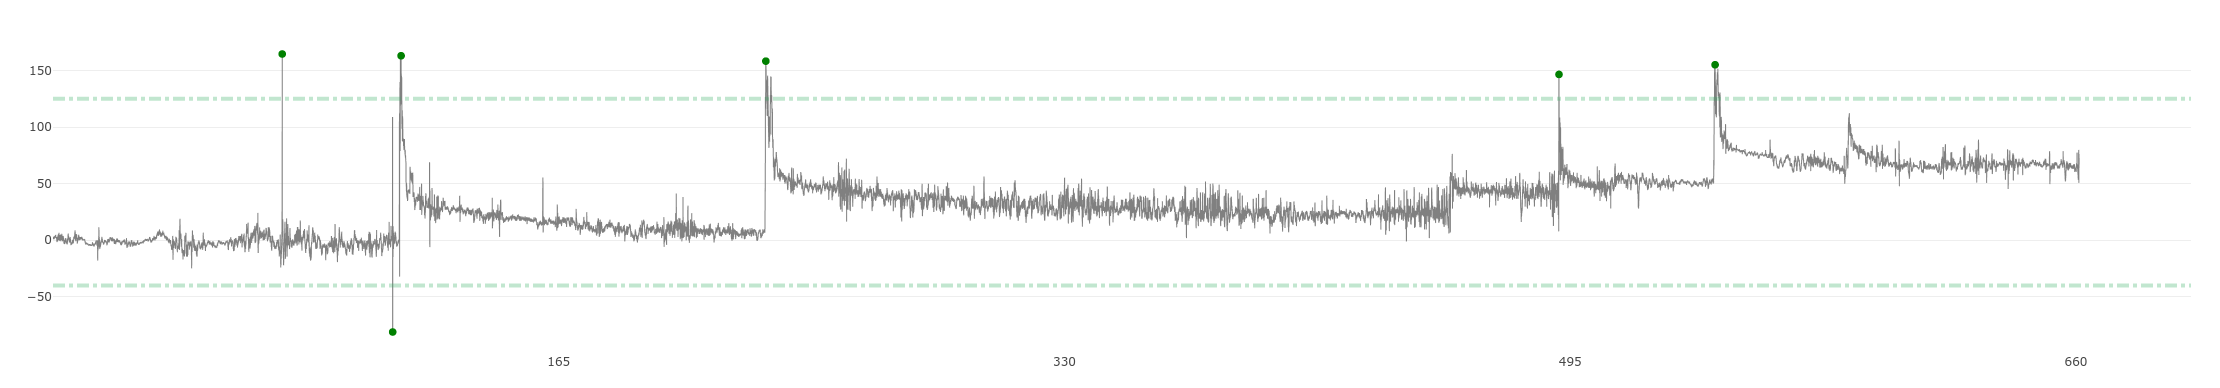
\includegraphics[width=1\linewidth]{gfx/timeseries_new.png}
    \caption{Zeitreihen im Vergleich}
    \label{fig:timeseries_compare}
\end{figure}
Der letzte Graph, der bereits in einer Webseite existiert, sind die Fingerprints. Durch die Reduzierung der verschiedenen Elemente des Graphen konnte gleichzeitig ein deutlich geordneterer und informativerer Graph erstellt werden. In dem Graphen, der in dieser Arbeit erzeugt wurde, können anstatt einer alle drei Raumrichtungen dargestellt werden. Ebenso wird durch das Data-Storytelling direkt sichtbar, welcher Punkt im Graphen die Zahl Eins erreicht hat. Dadurch kann schneller erkannt werden, bei welcher Messung die kritische Leistung erreicht wurde. In Abbildung \ref{fig:fingerprints_compare} ist der Vergleich zu betrachten.\\\\ 
\begin{figure}[!h]
    \centering
    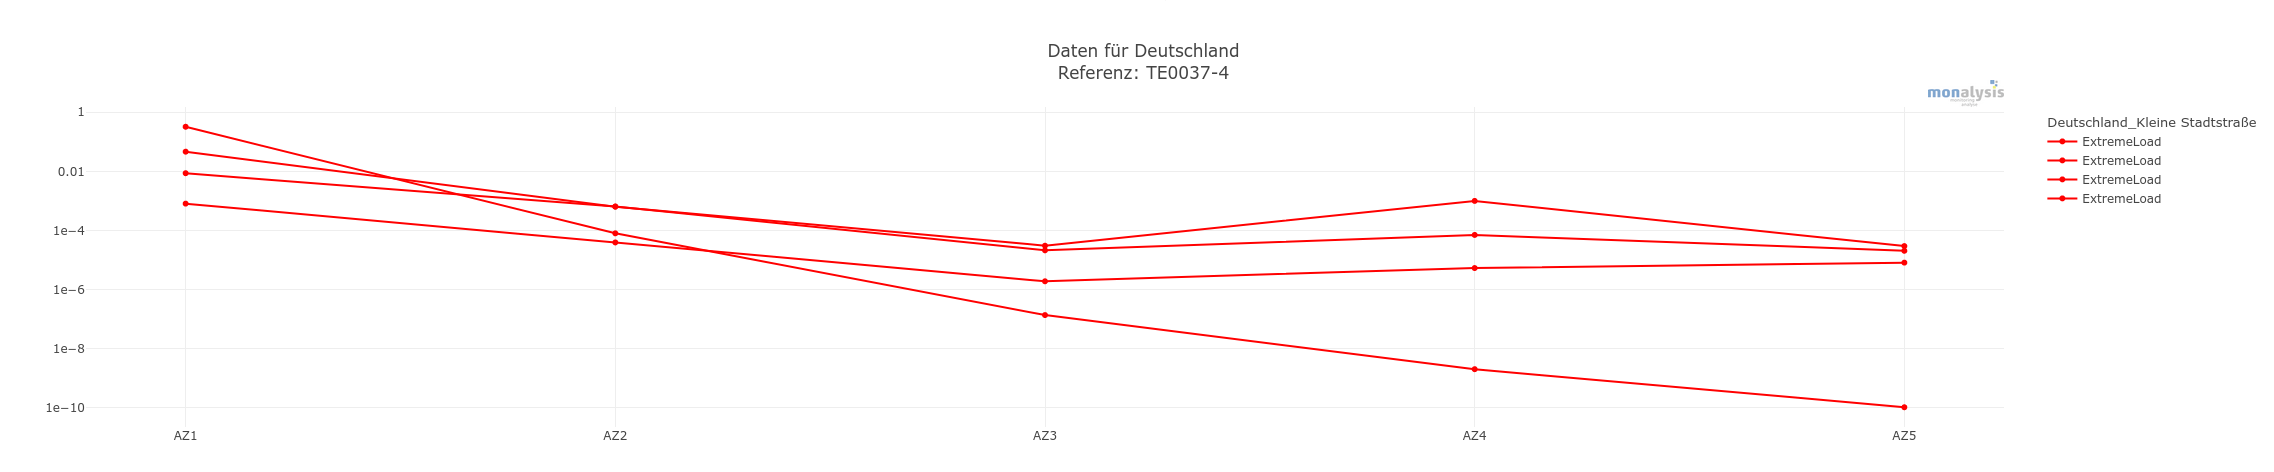
\includegraphics[width=1\linewidth]{gfx/fingerprints_old.png}
        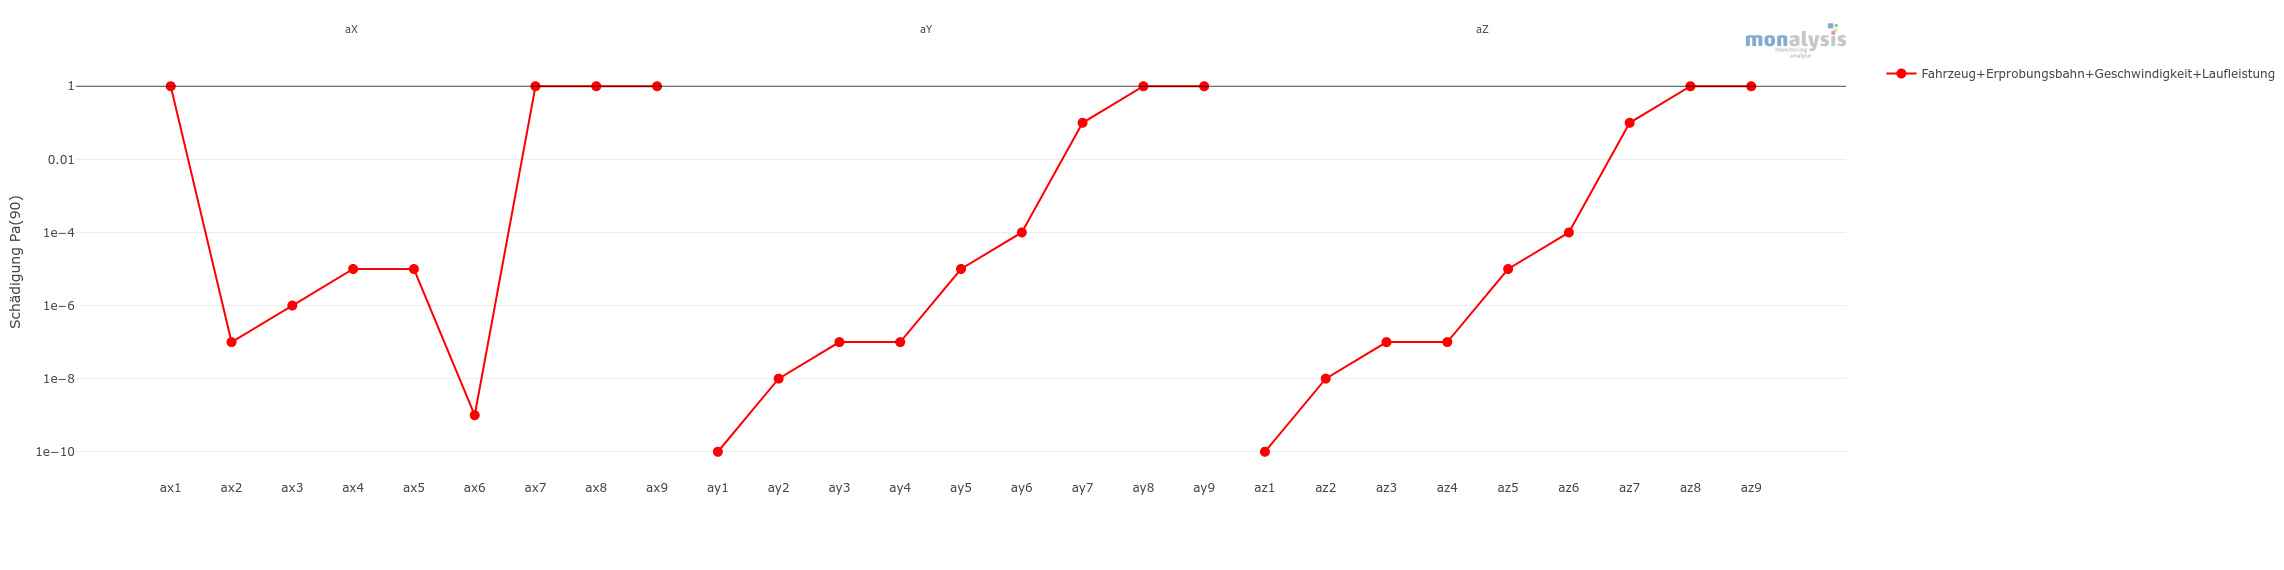
\includegraphics[width=1\linewidth]{gfx/fingerprints_new.png}
    \caption{Fingerprints im Vergleich}
    \label{fig:fingerprints_compare}
\end{figure}
\noindent
Durch diese Gegenüberstellungen lässt sich gut erkennen, dass das Data-Storytelling ein wertvolles Werkzeug ist, um Graphen informativ und Daten für den Benutzer verständlich darzustellen. Für Benutzer, die im Thema Betriebsfestigkeit und Fahrzeuge keine Experten sind, ist das Data-Storytelling wichtig, da sich durch den Einsatz des Storytellings lenken lässt, was der Benutzer als Erstes wahrnimmt.  
\section{Umfrage zu den Data-Storytelling-Graphen}
Zur Beurteilung des Data-Storytellings wurden die Experten aus dem Interview am Anfang der Arbeit zur Erkennung der Trends erneut interviewt. Dabei ist das Interview mit Jeele Böggemann in Anhang \ref{appendix:interview_ende_boeggemann}, das Interview mit Benedikt Mundl in Anhang \ref{appendix:interview_ende_mundl}, das Interview mit Michael Städele in Anhang \ref{appendix:interview_ende_staedele} und das Interview mit Florian Zenzinger in Anhang \ref{appendix:interview_ende_zenzinger} zu finden. Ihnen wurden die Graphen aus der entwickelten Webseite gezeigt sowie Fragen aus dem Interviewleitfaden in Anhang \ref{appendix:interview_ende} gestellt. Zur Auswertung der Interviews wurde erneut nach den Methoden von \cite{Mayring.2022}, \cite{Kuckartz.2022} und \cite{AndreMorgensternEinenkel.2023} eine inhaltlich strukturierende qualitative Inhaltsanalyse erstellt. Insgesamt sind sich die Experten einig, dass das Data-Storytelling eine deutliche Verbesserung der Graphen sowohl visuell, im Sinne des einfacheren Verstehens, als auch in der Geschwindigkeit, mit der die Graphen analysiert werden können, erreicht hat. Zu der Geschwindigkeit der Analyse mit Data-Storytelling äußern sich Jeele Böggemann in den Zeilen \lref{appendix:interview_ende_boeggemann:schneller}--770 und \lref{appendix:interview_ende_boeggemann:schneller_2}--786, Benedikt Mundl in den Zeilen \lref{appendix:interview_ende_mundl:geschwindigkeit}--839, Michael Städele in den Zeilen \lref{appendix:interview_ende_staedele:schneller}--926 und \lref{appendix:interview_ende_staedele:schneller_2}--941 sowie Florian Zenzinger in den Zeilen \lref{appendix:interview_ende_zenzinger:schneller}--992 und \lref{appendix:interview_ende_zenzinger:schneller_2}--1002. Alle vier Experten sind sich einig, dass die Analysen schneller durchgeführt werden können. Zu der Vereinfachung der Analyse der Graphen erklären Benedikt Mundl (Zeilen \lref{appendix:interview_ende_mundl:leichter}--862) und Michael Städele (Zeilen \lref{appendix:interview_ende_staedele:leichter}--933), dass es besonders bei Benutzern, die noch wenig versiert mit den Daten umgehen können, eine große Hilfe ist, Data-Storytelling zu benutzen. Dieser Aussage stimmt auch Florian Zenzinger in der Zeile \lref{appendix:interview_ende_zenzinger:leichter} zu, wobei er anmerkt, dass die Graphen „deutlich übersichtlicher“ seien.\\ Zudem stimmen alle Experten überein, dass das Data-Storytelling auch in Zukunft auf weitere fahrzeugbasierte Daten angewandt werden soll beziehungsweise in bereits vorhandenen Projekten nachträglich implementiert werden soll (Jeele Böggemann: Zeile \lref{appendix:interview_ende_boeggemann:neue}, Michael Städele: Zeilen \lref{appendix:interview_ende_staedele:neue}--920, Benedikt Mundl: Zeilen \lref{appendix:interview_ende_mundl:neue}--833, Florian Zenzinger: Zeile \lref{appendix:interview_ende_zenzinger:neue}). Als Nachteil wird von dem Experten Benedikt Mundl (Zeilen \lref{appendix:interview_ende_mundl:nachteil}--876) die Schwierigkeit beim Finden von verständlichen Umschreibungen für manche Funktionen der Trenderkennung erwähnt. Dieser Nachteil wird mit der Einführung von Beispielen in dem Trenderkennungsmenü ausgeglichen. Von Michael Städele (Zeilen \lref{appendix:interview_ende_staedele:nachteile}--954) wird als Nachteil genannt, dass bei der Erkennung von Trends ein gewisser Konfigurationsaufwand entsteht, besonders bei den Einstellungen der Trenderkennung. Die Vorteile des Data-Storytellings werden von Michael Städele (Zeilen \lref{appendix:interview_ende_staedele:story}--910 und \lref{appendix:interview_ende_staedele:story_2}--941) zusammengefasst als „schnellere Möglichkeit, damit zu arbeiten“ und als „Fokussierung auf die wichtigen Werte“. Diese Vorteile werden auch von Benedikt Mundl (Zeilen \lref{appendix:interview_ende_mundl:story}--862) genannt. Insgesamt sind alle Experten der Meinung, dass das Data-Storytelling in dieser Arbeit erfolgreich war.
\section{Fazit}
Das Ziel dieser Arbeit war festzustellen, ob das Data-Storytelling einen Mehrwert für komplexe fahrzeugbasierte Daten bieten kann.
Zunächst wurde der Prozess des Data-Storytellings genauer analysiert, und im Anschluss wurden mehrere Experteninterviews durchgeführt, um die passenden Informationen zu identifizieren. Da es sich bei dem letzten Punkt des Data-Storytellings um das Erzählen einer Geschichte handelt, ist es wichtig zu verstehen, weshalb welche Informationen in den Daten von Bedeutung sind. Anhand der Ergebnisse des Experteninterviews wurde eine Trenderkennung implementiert, die dazu genutzt werden kann, verschiedene interessante Punkte in den Daten, wie minimale oder maximale Punkte, sowie verschiedene über längere Zeit anhaltende Verhalten zu charakterisieren. Anhand der Ergebnisse der Trenderkennung können mit dem Data-Storytelling Geschichten entwickelt werden. Zudem wurde in dieser Arbeit der Prozess des Data-Storytellings an mehreren Graphen angewendet und je nach Ziel des Graphen angepasst. Diese Graphen konnten mit bereits existierenden Graphen, die einem ähnlichen Zweck dienen, verglichen werden. Hierdurch ist klar zu erkennen, dass die Graphen, die durch den Data-Storytelling-Prozess aufbereitet wurden, leichter zu verstehen sind und schneller entscheidende Inhalte der Visualisierung zu erkennen sind. Diese These wurde von den bereits am Anfang interviewten Experten bestätigt. Von den Experten wurde auch klar formuliert, dass sich das Data-Storytelling gut für fahrzeugbasierte Daten eignet und weiterhin auf diese Daten angewendet werden soll. Obwohl das Data-Storytelling für einige Graphen eine große Bereicherung ist, kann es für einige Anwendungsfälle schwierig sein, die passende Geschichte oder den passenden Call-To-Action zu definieren. Dabei ist hauptsächlich zu beachten, ob der Graph zu reinen Beobachtung von Daten genutzt werden soll, oder ob tatsächlich eine Aussage aus den Daten hervorgeht. Trotzdem kann man mit den ersten drei Schritten des Prozesses des Data-Storytelling nahezu jeden Graphen verbessern. Auch ist aus dieser Arbeit hervorgegangen, dass die Art der Daten, die beim Data-Storytelling dargestellt werden, eine sehr große Rolle spielen. Die Erstellung der Graphen ist sehr individuell, was besonders beim Erzählen der Geschichte aufgefallen ist. Deswegen wäre es interessant, das Data-Storytelling in Zukunft auch auf andere Daten angewendet zu sehen, besonders da jeder Anwendungsfall einzigartig ist. 

%*************************************************************************
% Backmatter
%*************************************************************************
\appendix
\cleardoublepage
\part{Appendix}
\chapter{Experteninterview zu Trends in den Daten}
\section{Interviewleitfaden}
\label{appendix:interview_trends}
\begin{description}
\item[Forschungsfrage]\hfill \\\\
Welche Trends sind in Bezug auf die Daten für den Kunden von Interesse?\\
\item[Einstieg]\hfill \\\\
Die Interviews dienen dazu, mithilfe der Experten zu erforschen, welche Trends in den Daten durch das Data Storytelling dargestellt werden sollen.
Kurzer Einstieg in das Thema der Masterarbeit und Erklärung der Forschungsfrage und dem Zweck des Interviews.\\
\item[Hauptteil]\hfill \\\\
Welche Daten werden von den Sensoren geliefert?\\
Worauf achten Sie, wenn Sie die Daten analysieren?\\
Im Bezug auf die bereits geplanten Unterseiten\\
\begin{itemize}
    \item Datenbasis\hfill \\Ein Dashboard, das einen Überblick über die vorhandenen Fahrzeuge und Flotten geben soll
    \item Überwachung Dauerlauferprobung\hfill \\Eine Seite zur Analyse von einer einzelnen Fahrt während der Dauerlauferprobung, also eine Fahrt auf einer abgeschlossenen Strecke, wobei die Strecke, sowie der Untergrund immer gleich bleiben
    \item Vergleich von Einsatzdaten\hfill \\Eine Seite, die zur Auswahl von zwei verschiedenen Eingaben genutzt werden kann, um diese zu vergleichen\\
\end{itemize}
sind welche Visualisierungen oder Informationen in den Daten interessant?\\
\item[Rückblick und Zusammenfassung]\hfill \\\\
Insgesamt stimmen die Interviews, sowie die Workflows und Points of Interest aller interviewten Personen zum größten Teil überein. Daraus lässt sich zusammenfassen, dass für die Trends Aufstiege, Abstiege, Extremwerte, Offsets, Schwingungen und allgemeine Abweichungen hervorgehoben werden können. Ebenso können Defekte und Messfehler oder Fehler des Fahrers gekennzeichnet werden.

\end{description}
\section{Transkription Interview Benedikt Mundl}
\label{appendix:interview_trends_mundl}
Interviewpartner: Diplomingenieur (FH) Benedikt Mundl, seit 15 Jahren in der Messdatenanalyse mit Fahrzeugen und Flugzeugen\\
Datum: 6. November 2023, um 9 Uhr\\
Dauer des Interviews: 24 Minuten\\

\begin{linenumbers}
\noindent
I: Hallo Herr Mundl, vielen Dank, dass du dir für das Interview Zeit nimmst.\\\\
BM: Gar kein Problem, ich beantworte deine Fragen gerne.\\\\
I: Wie du schon weißt, besteht meine Masterarbeit aus dem Frontend der Webseite mit Verwendung von Data Storytelling und zusätzlich noch dem Definieren von mathematischen Regeln, mit denen ich Trends in unseren Daten erkennen kann, um die besser darzustellen.\\
Das heißt für mich ist es sehr interessant zu wissen, worauf ihr genau achtet, wenn ihr die Daten auswertet, wenn ihr euch die anschaut, ob es da irgendwelche Auf- und Abstiege gibt oder im Allgemeinen wie die Daten dargestellt werden sollen.\\\\
BM:\llabel{appendix:interview_trends_mundl:defekte_1} Ja, das heißt, es geht auch um so Dinge wie Messfehler oder ähnliches?\\\\
I: Zum Beispiel, ja.\\\\
BM: Okay, das ist eine sehr umfangreiche Frage.\\\\
I: Es ist ja auch eine Masterarbeit.\\\\
BM:\llabel{appendix:interview_trends_mundl:extremwerte_1} Also gut, wenn ich Daten zum ersten Mal sehe, dann schaue ich als Erstes auf den Wertebereich, heißt, entspricht, das, was da [von den Sensoren] ankommt, ungefähr dem, was zu vermuten ist. Was zu vermuten ist, das weiß man aus Erfahrung. Da kann man sich nicht genau auf eine Zahl festlegen, man muss halt wissen, okay, das sollte in so und so einem Bereich liegen.\llabel{appendix:interview_trends_mundl:defekte_2} Wenn jetzt bei einer Beschleunigung auf einmal fünf Pausen herauskommen, dann weiß ich schon, das ist Quatsch.\llabel{appendix:interview_trends_mundl:plausibilisierung_1} So, wenn die Schädigung dann irgendwo 5 g anzeigt, dann ist das für den ersten Eindruck in Ordnung, kann natürlich auch zu groß oder zu klein sein, aber für den ersten Moment ist die Zahl plausibel.\\ \llabel{appendix:interview_trends_mundl:peaks_1}Als Nächstes schaue ich mir an, ob ich auf den ersten Blick bereits einige Peaks sehe, irgendwelche Ausreißer, die deutlich über diesem gewünschten, oder anvisiertem Wertebereich liegt. Das sind dann immer mal Einzelwerte, die auf einmal irgendwo hinspringen, die sind dann durch beispielsweise defekte Sensoren bei der Datenerfassung selber aufgetreten. Das kann aus verschiedenen Gründen vorkommen, aber die Gründe sind ja erstmal egal, wir wollen diese Werte ja einfach nicht haben, in der Auswertung.\\ Und da fallen diese Werte dann relativ schnell auf, wenn man sich grafische Zeitschriebe ansieht, wenn man die Daten nur als reine Zahlen ansieht, sind diese Werte ziemlich schwer zu finden.\llabel{appendix:interview_trends_mundl:offset_1} Als Nächstes beschäftige ich mich mit Drifts. Drifts bedeutet bei uns, ein Kanal fängt bei einem Ausgangswert an, idealerweise 0, und verändert sich ganz langsam und stetig über das komplette Zeitsignal nach oben oder nach unten und endet dann bei einem neuen Offsetwert. Das passiert relativ häufig bei beispielsweise Temperaturwerten. Und dann schaue ich auf so Defaultwerte wie beispielsweise eine Samplingrate mit einem Hertzwert, sind die Einheiten korrekt, sind die Namen in Ordnung, diese Werte kann man auch als Metawerte bezeichnen. Ist das ungefähr die Antwort auf die Frage?\\\\
I: Ja, das hilft mir sehr weiter. Das war eine sehr ausführliche Antwort. Ich muss erstmal euren Prozess verstehen, um später die Darstellung im Data Storytelling so gutzumachen, dass euch dadurch Arbeit abgenommen werden kann.\\\\
BM: Ich habe mir mal ein Heft mit den verschiedenen Fällen, die bei der Analyse vorkommen können, angefertigt, das kann ich dir gerne zukommen lassen.\\\\
I: Ja, sehr gerne, das wäre sehr hilfreich!\\\\
BM: Kein Problem.\\\\
I: Wir haben ja bereits Unterseiten für unsere Webseite festgelegt. Worauf achtest du, wenn du die Daten in Bezug auf die einzelnen Unterseiten analysierst? Auf der ersten Seite, der Dashboard Seite, gibt es ja noch keine wirklichen Daten zu analysieren, keine Trends zu erkennen, oder?\\\\
BM:\llabel{appendix:interview_trends_mundl:dashboard_1}  Genau, da komme ich erstmal an und verschaffe mir einen Überblick. Damit ich weiß, wie viele Kilometer haben wir erfasst, mit welchen Autos, welche Autos sind überhaupt erstmal in der Analyse verfügbar. Einfach ein Gefühl, dafür kriegen, welche Datenbasis vorliegt. \\\\
I: Und bei der Überwachung Dauerlauferprobung?\\\\
BM:\llabel{appendix:interview_trends_mundl:dauerlauferprobung_1}\llabel{appendix:interview_trends_mundl:fahrer_1} Da wird es dann natürlich schon wichtig. Die Dauerlauferprobung soll eigentlich immer dasselbe sein. Also blöd gesagt, idealerweise würde man diese Dauerlauferprobung auf einem Prüfstand fahren, was aber realistisch nicht möglich ist, weil das technisch nicht funktioniert. Das wurde schon ausgetestet, aber man war nie erfolgreich. Also nicht mal nur monalysis, sondern wirklich große Firmen und Tariffunktionäre. Oder das sollte von Robotern auf dem Erprobungsgelände gefahren werden. Die tatsächlich immer gleich fahren. Beispielsweise die erste Strecke immer mit 25 km/h, die zweite Stecke immer mit 12,3 km/h. Geht theoretisch, ist aber natürlich schon eher teurer, bis mal so ein kompletter Roboterbetrieb auf einem Testgelände realisiert wurde. Besonders schwierig ist das Ganze, wenn der Roboterbetrieb mit verschiedenen Fahrzeugen betrieben werden soll. Von dem her wurde das von den Firmen noch nicht in der Gänze realisiert.\\ Also werden die Fahrzeuge von Fahrern gefahren. Das ist die aktuell günstigste Alternative.\llabel{appendix:interview_trends_mundl:fehler_1} Da ist allerdings das Problem, dass wenn ein Fahrer mehrere Wochen lang immer die gleiche Strecke fährt, einfach Inkonsistenzen dabei auftreten. Oder er kennt die Strecke bereits so gut, dass es genau weiß, wo beispielsweise Schlaglöcher sind und umfährt diese, um nicht durchgeschüttelt zu werden. Das ist problematisch, da die ganze Dauerlauferprobung dann inkonsistent wird. Das bedeutet, dass die gefahrene Dauerlauferprobung dann nicht mehr zu den Berechnungsgrundlagen passt, dass die Annahmen, wenn X km diese Erprobung gefahren wird, dann entspricht das dem Fahrzeug tatsächlich.\llabel{appendix:interview_trends_mundl:dauerlauferprobung_2} Das muss das Fahrzeug widerspiegeln, sonst gibt es keine Aussage, ob die Referenz, die gefahren wurde, überhaupt das widerspiegelt, was berechnet wurde. Deswegen ist es wichtig, die Dauerlauferprobung zu kennen, damit man kontrollieren kann, inwiefern die Strecke immer gleich gefahren wurde, und damit man direkt schon erkennen kann, ob Schäden aufkommen, weil wenn nachvollzogen werden kann, dass die Fahrer die Fahrzeuge immer gleich gefahren haben, aber der Verlauf der Dauerlaufüberwachung ändert sich plötzlich, dann ist das problematisch.\llabel{appendix:interview_trends_mundl:schädigungswerte_1}\llabel{appendix:interview_trends_mundl:dauerlauferprobung_3} Der Verlauf der Dauerlaufüberwachung wird widergespiegelt durch Schädigungswerte, das heißt für jede Strecke wird ein Schädigungswert ausgerechnet.\llabel{appendix:interview_trends_mundl:schädigungswerte_2} Beispielsweise, wenn der Belgisch Block korrekt befahren wird, dann ist Zahl X der standardmäßige Schädigungswert. Diese Werte kann man dann aufsummieren und anhand dessen kann man die Werte visualisieren.\llabel{appendix:interview_trends_mundl:aufstiege_1}\llabel{appendix:interview_trends_mundl:defekte_3} Wenn die Werte dann einen riesen Sprung darstellen, dann ist irgendwo ein Problem aufgetreten, das kann dann auch daran liegen, dass das Fahrzeug einen Defekt hat, weil man fährt diese Erprobung ja eigentlich nur, um zu wissen, ob das Fahrzeug das aushält. Also sind Schäden irgendwo vorprogrammiert. Es ist also keine Besonderheit, dass während der Erprobung mal ein Teil kaputtgeht. Es geht darum, an, die Grenze des Fahrzeugs zu kommen.\\ Und von dem her sind diese beiden Aspekte das Wichtige. Zum einen das Überwachen, wurde alles immer gleich gefahren. Und zum anderen können jetzt schon Schäden erkannt werden.\\\\ 
I: Vielen Dank, also so Hüpfer oder Anomalien ist ja das, wo Trends potenziell erkannt werden können.\\\\
BM:\llabel{appendix:interview_trends_mundl:defekte_4}\llabel{appendix:interview_trends_mundl:fehler_2}\llabel{appendix:interview_trends_mundl:fahrer_2} Ja, die können aber zwei Ursachen haben, schlechtes Fahren oder Defekte.\\\\
I: Die Ursachen sind erstmal gar nicht so wichtig, wichtig ist zu erkennen, da passiert etwas mit den Daten und das ist nicht ganz normal und das dementsprechend darzustellen.\\\\
BM:\llabel{appendix:interview_trends_mundl:abweichungen_1} Im Endeffekt, kann man schon bevor man losfährt, eine Prognose treffen, wie die Schädigung bei 10.000 km, 20.000 km und so weiter aussieht. Vom Gesamtschädigungswert. Und wenn das vom Soll abweicht, dann kommt es zu diesen Anomalien.\\\\
I: Okay, und dann noch zum Vergleich von Einsatzdaten, das ist die letzte Seite.\\\\
BM: Ja, das ist dann die eigentliche Analyse selber.\llabel{appendix:interview_trends_mundl:dauerlauferprobung_4} Weil da ist dann die Dauerlauferprobung geführt und das hat alles funktioniert. Und dann wissen wir, okay, das, was bei der Dauerlauferprobung gefahren wurde, das nennen wir Zyklus, es kann auch Erprobungsmaßstab genannt werden. Dieser Zyklus bedeutet, bis X Kilometern ist das Fahrzeug erprobt. Was danach passiert, das wissen wir nicht. Und dieser Zyklus wird dann auf 100 \% Belastung gesetzt. In der Betriebsfestigkeit ist das dann nicht 100 \%, sondern eine 1.\llabel{appendix:interview_trends_mundl:vergleich_1} Und deswegen werden dann die Schädigungswerte auf die 1 gelegt. Danach kann der Erprobungszyklus gespiegelt werden und für andere Strecken eingesetzt werden. Und diese Daten können dann gebündelt werden, um die neuen Einsätze im Vergleich zum Erprobungszyklus zu analysieren. Dadurch kann man die Schädigungen hoch multiplizieren, um eine Zahl zu berechnen, bei der die Schädigung des Erprobungszyklus erreicht ist. So kann entschieden werden, welche Einsätze relevant sind, und welche Komponenten werden, wann stark belastet, um beispielsweise Ersatzteile mit auf den Einsatz zu nehmen. So lässt sich auch eine ungefähre Aussage treffen, wann welche Komponenten versagen. Also soll in der Darstellung gezeigt werden, wie der gezeigte Einsatz im Vergleich zu der Auslegung, also der Dauerlauferprobung ist. Hierbei sollen aber auch andere Einsätze miteinander verglichen werden können. Die Frage ist, ob es dann auch möglich ist, zu sagen, wenn der Kunde auf diesen Einsatz aufbricht, sollte er dann bestimmte Ersatzteile mitnehmen, weil mit dem Ausfall von diesen gerechnet werden kann. Hier geht es dann richtig in das ingenieursmäßige Arbeiten rein, dass man lernen und verstehen muss, was man aus den Daten herausziehen kann. Das heißt, diese letzte Seite ist das Spannendste.\llabel{appendix:interview_trends_mundl:vergleich_2} Da können dann auch richtige Querverweise zu älteren Einsätzen getroffen werden. Dass zum Beispiel bei Neuentwicklungen bei dem Bauteil XY die Schädigung YZ vorgekommen ist, dann können auch beispielsweise ältere Daten bei ähnlichen Bauteilen verglichen werden, ob die Werte plausibel sind. Da kann es sogar sinnvoll sein, eine Einzelteilanalyse zu starten. \\\\
I: Sehr gut, sehr spannend. Was würdest du dir wünschen, wenn du dir eine Visualisierung anschaust?\\\\
BM:\llabel{appendix:interview_trends_mundl:extremwerte_2} Was ich unbedingt brauche, ist die minimal und maximale Schädigung, also die Extremwerte, ob als Linie oder als Balken, das ist mir egal. Aber auf jeden Fall als Diagramm, als Zahl ist das schwer einzuordnen, zu häufig zu viele Zahlen.\llabel{appendix:interview_trends_mundl:schädigungswerte_3} Was auch immer sehr, sehr hilfreich ist, sind Schädigungswerte, das hilft einfach enorm für das grobe Einschätzen von verschiedenen Messungen. Der sagt zwar nicht alles aus, so ein Schädigungswert, aber er ist sehr hilfreich, dass man für den Kontext der Messung einfach einen Überblick hast, ist das allgemein ein härterer oder weicherer Untergrund.\llabel{appendix:interview_trends_mundl:zaehlmethoden_1} Dann die Kollektive, Rangepair, Levelcrossing, die sind einfach in der Betriebsfestigkeit oder Auslegung das Mittel, mit denen können wir Ingenieure sehr gut arbeiten. Oder auch manchmal ein Time at Level, das ist so ein ähnliches Kollektiv. Also eine Verweil Aufzählung, wie lang ist der Zustand vorhanden. Also auf der y-Achse die Amplituden und auf der x-Achse die Zeit in Sekunden zum Beispiel. Gerade so Drehzahlen sind dafür gut geeignet.\llabel{appendix:interview_trends_mundl:zeitreihen_1} Und natürlich, wenn etwas heraussticht in den Graphen, dann sollte eine detaillierte Ansicht vorhanden sein. Und dafür werden eigentlich die Zeitreihen genutzt, weil anhand von den Zeitschrieb kann man sehr gut erkennen, was wann passiert ist.\llabel{appendix:interview_trends_mundl:wunsch_1} Und da wäre es sehr, sehr hilfreich, wenn man verschiedene Zeitschriebe vergleichen könnte. Das ist dann aber ziemlich aufwändig, weil man dafür auch die Geschwindigkeit im Betracht ziehen muss. Ansonsten werden ja bei jedem Rad beispielsweise getrennt die Werte erfasst, und wenn aber die Kanäle sehr unterschiedlich sind, dann sollte man diese vergleichen können, um zu sehen, ob die Unterschiede noch in einem realistischen Bereich sind. Also so Querverweise zwischen verwandten Messstellen. Dann vielleicht noch die Geschwindigkeit und GPS, falls vorhanden. Oder die Querbeschleunigung, um an einem Rundkurs herzuleiten, an welcher Stelle man sich befindet. So etwas in Richtung Location. Damit lässt sich das Ganze gut zusammenfassen.\\\\
I: Okay, dann vielen Dank für deine Zeit und noch einen schönen Tag.\\\\
BM: Danke gleichfalls.
\end{linenumbers}

\section{Transkription Interview Jeele Böggemann}
\label{appendix:interview_trends_boeggemann}
Interviewpartner: Bachelor of Engineering Jeele Böggemann, seit 6 Jahren in der Messdatenanalyse mit Fahrzeugen und Flugzeugen\\
Datum: 13. November 2023, um 13 Uhr\\
Dauer des Interviews: 15 Minuten\\

\begin{linenumbers}
\noindent
I: Hallo Jeele, danke dass du dir Zeit für das Interview nimmst. Erstmal möchte ich dir gerne das Thema meiner Masterarbeit erklären. Es geht darum das Frontend des neuen Kundenprojekts mit Data Storytelling zu bauen. Hast du Data Storytelling schon mal gehört?\\\\
JB: Nein, das sagt mir noch nichts.\\\\
I: Okay, das ist eine Art, wie man Graphen erstellt. Dass man quasi eine Geschichte im Graphen erzählt und mein Ziel ist, damit eigentlich die ganze Bedienung der Seite zu erleichtern. Also automatisch Auf- und Abstiege erkennt und die dann extra hervorhebt. Genau, deswegen wäre es für mich sehr spannend, worauf du achtest, wenn du die Daten über das Frontend anschaust.\\\\
JB: Ah, ich verstehe.\\\\
I: Gut, dann starten wir gleich mal. Bei den Daten, welche Daten werden da genau von den Sensoren geliefert?\\\\
JB: \llabel{appendix:interview_trends_boeggemann:daten_1}Okay, da haben wir \ac{DMS}, mehrere, an den Federbeinaufhängungen, da sind an der Vorderachse und an der Hinterachse jeweils vier, schräg gegenüber voneinander. Dann sind an der Spurstange, an dem Lenkgestänge sind noch welche appliziert. Generell, am Fahrwerk sind \ac{DMS}, am Fahrersitz wird noch die Beschleunigung aufgezeichnet. In alle drei Richtungen, plus die Ableitung dazu, also die Drehraten um die Achsen.\\\\
I: Okay, und wenn du dir das jetzt mal so vorstellst, wie das im Porsche Frontend aussieht. Worauf achtest du, wenn du dir die Daten anschaust?\\\\
JB:\llabel{appendix:interview_trends_boeggemann:abweichungen_1}\llabel{appendix:interview_trends_boeggemann:extremwerte_1} Ich schaue mir als allererstes Mal die Extremwerte an, um zu sehen, ob da Ausreißer drin sind.\llabel{appendix:interview_trends_boeggemann:abweichungen_2}\llabel{appendix:interview_trends_boeggemann:defekte_1} Wenn mir da ein Wert auffällt, weil er aus dem Rahmen fliegt, dann schaue ich mir die dazugehörige Zeitreihe an, um zu plausibilisieren, ob der Wert echt ist, oder ob das ein Messfehler ist.\llabel{appendix:interview_trends_boeggemann:abweichungen_3}\llabel{appendix:interview_trends_boeggemann:schädigungswerte_1} Sowas Ähnliches mache ich dann mit den Schädigungen auch, also ich prüfe, ob die alle in einem ähnlichen Bereich sind, also entweder aus Erfahrung oder aus ähnlichen Fahrzeugen. Weil mittlerweile gibt es auch eine recht große Basis an Altmessungen. Die auch immer zum Gegenchecken verwendet werden kann. Und wenn dann irgendwo etwas Auffälliges ist, heißt die Werte sind zu hoch oder zu niedrig, dann geht es in den vertiefteren Vergleich zu den alten Fahrzeugen oder es wird geschaut, wie wurden denn überhaupt auf der Strecke gefahren. Ab und zu schaue ich mir auch Videos an von der Rennstrecke, um einfach die Kurven zu sehen. Um abschätzen zu können, was in der Kurve passiert. Kann das alles sein? Und dann ist es je nachdem was für eine Auswertemethode benutzt wird. Wenn jetzt konventionell ausgewertet wird, also nur ein Outing genommen wird und dass das irgendwohin extrapoliert wird, dann bin ich eigentlich fertig mit der Auswertung und wenn Rennsportmethode ausgewertet werden soll, dann werden noch die Streuungen beobachtet. Da gibt es dann von dem Kunden eine Vorgabe, wie hoch die Streuung sein darf und wenn ich über den Wert komme, dann werden nochmal einzelne Runden vergleichen, um zu entscheiden, ob die Schädigung nach oben, also das wird dann etwas konservativer ausgewertet oder festlege, dass die hohen Streuungen eher Ausreißer sind und die Schädigung weiter nach unten schiebe. \\\\
I: Vielen Dank, und gibt es dann auch so Trends oder sowas auf die du achtest bei den Daten selber?\\\\
JB: Eigentlich weniger.\\\\
I: Also das sind dann wirklich diese Ausreißer, die dich interessieren? Sind die dann spannend oder eher unschön, weil man sie vermeiden möchte?\\\\
JB:\llabel{appendix:interview_trends_boeggemann:daten_2}\llabel{appendix:interview_trends_boeggemann:fahrer_1} Kommt ganz darauf an. Kommt immer darauf an, wie das Fahrzeug ausgelegt ist, auch wo mein Target liegt. Also quasi der Wert, mit dem das Fahrzeug abgeprüft worden ist. Wenn ich da irgendwo darunter liege, ist die Messung in Ordnung.\llabel{appendix:interview_trends_boeggemann:abweichungen_4} Wenn ich über dem Target darüber liege, muss man auch nochmal genauer in die Daten gehen.\llabel{appendix:interview_trends_boeggemann:fehler_1} Und dann wird irgendwo auch eine Entscheidung getroffen, ob die Messung repräsentativ ist, ob das Fahrzeug das abkönnen muss, was da in der Fahrt passiert. Oder geht das eher Richtung Missuse.\\\\
I: Und die Targets werden dann vom Kunden festgelegt, oder?\\\\
JB:\llabel{appendix:interview_trends_boeggemann:daten_3} Genau, also normalerweise sind die Targets schon fertig, bevor wir mit dem Testen anfangen. Das ist eher eine Ausnahme, dass man das im Nachhinein festlegt. \\\\
I: Also wir haben ja für das Frontend schon Unterseiten festgelegt für das Frontend. Da haben wir einmal die Datenbasis, also quasi ein Dashboard, dass man schonmal weiß, welche Fahrzeuge es gibt und wie viel die fahren. Da gibt es ja noch keine Visualisierung. Gebe es da irgendwas was du als Visualisierung spannend fändest als Benutzer?\\\\
JB: Was jetzt anders als bei Porsche ist?\\\\
I: Darf anders als bei Porsche sein. Es gibt dann auch noch die anderen Unterseiten, also die nächste ist die Überwachung Dauerlauferprobung.\\\\
JB:\llabel{appendix:interview_trends_boeggemann:dauerlauferprobung_1} Ja, okay, also bei dieser Auswerteseite, die ist ja mehr oder weniger so gewachsen, wie ich oder wir die gerne hätte. Daher fällt mir da so spontan nichts ein, was ich da gerne anders hätte. Weil die ja aus der Erfahrung raus, wie wir Auswerten entstanden ist. Es gibt halt dann den Schnellzugriff auf die Einzelrunden, um halt schnell einen Extremwert zu plausibilisieren. Was da noch interessant wäre, wenn man zwei Runden miteinander vergleichen könnte.\\\\
I: Ja gut, also bei dem Kunden ist es ja so, dass man die Dauerlauferprobung hat und dann als zweite Seite den Vergleich von Einsatzdaten. Also das ist dann schon als eigene Seite mitberücksichtigt. \\\\
JB:\llabel{appendix:interview_trends_boeggemann:zaehlmethoden_1}  Die Kollektive kann man auch direkt sehen. Nein, da fällt mir echt nichts ein, was da irgendwie noch gebraucht wird. Ich komme ja da eigentlich recht schnell an alle Informationen ran, die ich brauche.\\\\
I: Okay, an sich möchte ich ja mit der Masterarbeit die Graphen so weiterentwickeln, dass die euch schon Arbeit abnehmen, dass ich als die Daten bekomme und schon erkenne, okay, hier passiert etwas Komisches und dann kann ich das direkt farbig darstellen und die anderen Daten, bei denen nichts Gruseliges passiert, werden als Kontext dargestellt.\\\\
JB:\llabel{appendix:interview_trends_boeggemann:wunsch_1} Oh okay, also was da vielleicht hilfreich sein könnte, wäre, wenn man die Balkendiagramme noch sortieren könnte. Von groß nach klein.\\\\
I: Also einfach von den Werten dann?\\\\
JB: Genau.\\\\
I: Ich bin mir noch gar nicht sicher, ob das überhaupt Balkendiagramme bleiben, vielleicht wird das auch was ganz was Neues. Ich fange bei den Graphen von null an, also, falls du irgendwelche Ideen oder Wünsche hast, was als Benutzer cool wäre, was dir die Arbeit erleichtern würde, kannst du mir jederzeit Bescheid geben.\\\\
JB:\llabel{appendix:interview_trends_boeggemann:wunsch_2} Ja, vielleicht, was helfen könnte, da müsste ich aber auch nochmal mehr darüber nachdenken, wären mehr Hovereffekte.\\\\
I: Auf jeden Fall.\\\\
JB:\llabel{appendix:interview_trends_boeggemann:extremwerte_2}\llabel{appendix:interview_trends_boeggemann:wunsch_3} Das, wenn es quasi über eine Runde geht, man dann einen Extremwert hat, also das haben wir auch schon häufiger gemacht in anderen Auswertungen, wie oft kommt dieser Extremwert oder halt nahe diesem Extremwert das Ganze vor. Sodass man nicht erst ins Kollektiv schauen muss, sondern irgendwo mit der Maus darüber hovern, und dann sieht man, dass es da beispielsweise 20 Kilonewton sind und zwei Prozent weniger kam auch noch so oft in den Daten vor.\\\\
I: Ja zum Beispiel sowas. \\\\
JB:\llabel{appendix:interview_trends_boeggemann:abweichungen_5} Dann könnte man auch leichter entscheiden, ob das ein Ausreißer ist, oder ob der [Fahrer] die Runde halt einfach so gefahren ist.\\\\
I: Das ist genau so etwas, dass ich suche, so Trends um die Ausreißer zu erkennen.\\\\
JB:\llabel{appendix:interview_trends_boeggemann:offset_1} Dann gibt es ja noch mehrere so statistische Kennwerte, die man aus den Daten auslesen kann, wie zum Beispiel ein Median, das wäre vielleicht interessant, um zu erkennen, ob das ganz über die Zeit weg gedriftet ist, oder ob da ein Offset eingegeben ist. Das wäre dann Richtung plausibilisieren, und gar nicht mehr so Richtung analysieren. Aber ansonsten müsste ich da echt noch länger drüber nachdenken. \\\\
I: Alles gut, das hat mir schon sehr weitergeholfen. Du kannst dich ja auch gerne jederzeit melden, wenn dir in der Benutzung etwas auffällt. Dann danke ich dir auf jeden Fall sehr für deine Zeit und wünsche dir noch einen schönen Tag.\\\\
JB: Danke gleichfalls.
\end{linenumbers}
\section{Transkription Interview Michael Städele}
\label{appendix:interview_trends_staedele}
Interviewpartner: Diplomingenieur (FH) Michael Städele, seit 2008 in der Messdatenanalyse mit Fahrzeugen und Flugzeugen mit Betriebsfestigkeit\\
Datum: 16. November 2023, um 9 Uhr\\
Dauer des Interviews: 15 Minuten\\

\begin{linenumbers}
\noindent
I: Hallo, Herr Städele, vielen Dank, dass du dir für das Interview Zeit nimmst. Wie du ja schon weißt, geht es bei dem Thema meiner Masterarbeit um das Frontend des neuen Kundenprojekts. Und zwar, darum, dass man die Graphen mit Data Storytelling darstellt. \\\\
MS: Ja, kein Problem.\\\\
I: So, beim Data Storytelling ist es ja so, das ist eine Art, wie Daten dargestellt werden können. Dass aus den Daten eine Geschichte erzählt wird und euch, wenn ihr Daten auswertet, die Arbeit erleichtern wird. Soweit das möglich ist. Und meine Forschungsfrage ist in dem Sinne, welche Trends es in den Daten gibt, die man erkennen könnte, um die darzustellen, um euch zu helfen.\\\\
MS: Welche Trends?\\\\
I: Genau, also sowas wie hier ist die Schädigung hochgegangen oder heruntergegangen, und damit ich das gleich hervorheben kann, damit ihr gleich seht, was für euch spannend ist.\\\\
MS: Also rein auf Basis erstmal von der erfassten Daten?\\\\
I: Von den erfassten Daten, genau. Und rein darauf ausgelegt, was ihr interessant findet beim Auswerten.\\\\
MS:\llabel{appendix:interview_trends_staedele:aufstiege_1}\llabel{appendix:interview_trends_staedele:schädigungswerte_1} Also rein in den Daten, wenn man sich die anschaut, da ist ja immer, wenn eine hohe Amplitude ist, also wenn es hochgeht, dann ist die Schädigung immer relativ hoch.\llabel{appendix:interview_trends_staedele:abstiege_1} Wenn es niedrig ist, dann ist es immer im Verhältnis niedrig.\llabel{appendix:interview_trends_staedele:storytelling_1} Jetzt ist ja die Sache, die interessant ist, wie verhält sich der tatsächliche Einsatz, zu dem, was die Fahrzeughersteller oder eben auch der Kunde erprobt. Das heißt, einmal muss man irgendwie sehen, was macht der Kunde auf seinem Testgelände, Schädigungs-mäßig, und wie verhält sich das Ganze zu dem tatsächlichen Einsatz. Und wo im Einsatz ist es extrem hart, also zum Beispiel in welche Regionen, aber auch vielleicht welche Fahrweisen, welche besonderen Vorkommnisse könnten da einen Einfluss haben. Also ich sage jetzt einfach mal in dem Fall des Kundens, wenn die Gefahrenlage relativ gering ist, dann denke ich, wird da nicht so viel passieren, weil man dann sehr gemütlich fahren kann, wenn jetzt die Gefahrenlage sehr hoch ist, könnte es auch sein, dass auch auf Strecken, die vielleicht nicht so ganz schlimm sind, trotzdem hohe Belastungen auftreten können, weil der Fahrer übelst Gas geben muss. Was könnten die Daten noch so erzählen?\llabel{appendix:interview_trends_staedele:storytelling_2} Wie denn auch die Fahrbahn beschaffen ist, das heißt, wenn ich auf einem guten Asphalt fahre, dann wird da natürlich nicht so viel passieren, wie wenn ich auf einem Schotterweg fahre. Oder irgendeinem tiefen Gelände. Auch wenn da die Geschwindigkeiten relativ gering sind. Also kann man auch, je nach Region, irgendwo Rückschlüsse ziehen auf die Topologie von dem Land. Und dann ist auch noch eine Sache, die sehr interessant sein könnte, wie verhalten sich verschiedene Einsatzzwecke untereinander. Beispielsweise ganz normale Einsatzfahrzeuge und Fahrschulfahrzeuge. Ja, das sind so Sachen, die mir so auf die Schnelle einfallen, die solche Daten erzählen könnten.\\\\
I: Sehr gut, ich habe auch noch ein paar andere Fragen mitgebracht.\\\\
MS: Okay.\\\\
I: Welche Daten werden von den Sensoren genau geliefert?\\\\
MS:\llabel{appendix:interview_trends_staedele:daten_1} Also von den Sensoren im Fahrzeug werden geliefert, also die wir da zusätzlich erfassen, sind im Endeffekt Beschleunigungssignale im Fahrzeuginnenraum, in den drei Richtungen, also x, y, z und ich glaube, es sind auch noch die drei rotatorischen, also die Momente um x, y, z mit dabei. Und ansonsten haben wir wahrscheinlich noch Zugriff auf Fahrzeug-interne Sensorik, relativ einfache, ich kann aktuell noch nicht genau sagen, welche, ob dann da Lenkwinkel, oder eine Bremspedalstellung, oder ein Gang oder eine Geschwindigkeit, dabei sind. Und wünschenswert wäre noch GPS, aber das weiß ich noch nicht, ob das möglich ist. Das ist so das was geliefert wird und im Erprobungsprozess, also wenn die Fahrzeuge auf dem Testgelände fahren, werden meistens noch \ac{DMS} mit angeschlossen. Also wirklich, um dann die Kräfte an den einzelnen Komponenten zu messen. Und das ist dann der Zweck mit dem \ac{DT}, dass man das später nicht mehr messen muss, sondern nur noch an den anhand von den Beschleunigungen ableiten kann.\\\\
I: Alles klar, worauf achtest du, wenn du die Daten auswertest? Gibt es da einen Workflow, oder Points of Interest in den Graphen, die besonders spannend sind?\\\\
MS:\llabel{appendix:interview_trends_staedele:defekte_1} Also das allererste, was wichtig ist, ist überhaupt mal die Plausibilisierung von den Daten. Die ganze Messtechnik, die schon noch ganz schön fehleranfällig. Das ist nicht nur bei uns so, sondern generell, dass da einfach irgendwelche kurzen Sensorfehler oder irgendwelche Pikser drin sein können, das heißt es ist wichtig, dass die da eigentlich raus sind. Dass man die vorab erkennt, bevor man die wirkliche Auswertung macht.\llabel{appendix:interview_trends_staedele:aufstiege_2}\llabel{appendix:interview_trends_staedele:peaks_1} Und wenn ich jetzt einfach eine Zeitreihe anschaue, dann sind immer interessant, eigentlich hohe Ausschläge. Also gerade, wenn irgendwo recht hohe Belastungen auftreten, dann ist da ja irgendwo erstmal was Größeres passiert, als beim normalen Fahren.\llabel{appendix:interview_trends_staedele:schwingungen_1} Und was auch noch so ein Punkt ist, ist so ein bisschen so eine Trennung von dem Höher und Niederfrequenten Zeug, von so Fahrmanöver-Geschichten und auch von höherfrequenteren Sachen, die dann eher durch die Fahrbahnunebenheit hervorgerufen werden. Ja, und sonst, rein so optisch, wenn ich mir irgendwas anschaue, dann schaut man ja immer auf was, was markiert ist. Wenn ich mir eine Strecke anschaue, dann schaue ich ja auf Daten, die mit einer Signalfarbe 
hervorgehoben werden. \\\\
I: Genau, das versuche ich ja herauszufinden, was ich am besten hervorhebe. Beziehungsweise zu was für einer Konklusion ich auch kommen kann durch die Daten, die ich automatisch berechnen lassen kann, in dem ich mir so Trends überlege. \\\\
MS:\llabel{appendix:interview_trends_staedele:schädigungswerte_2} Was wir ja natürlich auch machen, sind den Zeitreihen ja die Schädigung abzuleiten. Dann gibt es ja zum Beispiel auch so Schädigungsevolutionen. Also einfach, wo dann über der Strecke oder der gefahrenen Zeit dann die Schädigung aufgetragen ist. Und da ist ja auch immer, wenn es irgendwo hochgeht, immer sehr interessant.\\\\
I: Also das wäre so ein Punkt, den du gerne hervorgehoben hättest?\\\\
MS:\llabel{appendix:interview_trends_staedele:peaks_2} Ja, ja, oder das ist die Frage wie man es dann zusammen bringt, mit einer Karte, oder? Das man sieht okay und hier ist es gerade besonders. Aber vom Prinzip her, wenn irgendwo was Höheres ist, dann ist es da interessant. \\\\
I: Also höher als jetzt der Durchschnitt?\\\\
MS: Als der Durchschnittswert zum Beispiel, genau. \\\\
I: Alles klar. Gut, und wir haben ja schon Unterseiten festgelegt, für die Webseite. Und da würde mich interessieren, was für Visualisierungen und/oder Informationen allgemein besonders spannend  wäre, für dich als auswertende Person. Und zwar haben wir ja die Datenbasis, da ist es ja an sich so, dass es noch gar keine Visualisierungen gibt, das ist ja nur so ein Überblick.\\\\
MS: Genau.\\\\
I: Das hatte ich auch so weiter geplant, dass es da noch keine Graphen gibt.\\\\
MS: Aber zum Beispiel in der Datenbasis, ich weiß nicht genau, was du unter Visualisierungen verstehst, aber die Fahrzeugbilder und sowas sind ja dann da auch drin, oder?\\\\
I: Ja, ich rede von Graphen.\\\\
MS: Ah, okay.\\\\
I: Dann die Überwachung Dauerlauferprobung, da wird es ja dann schon spannender.\\\\
MS: Was ich da gerne sehen würde? In der Überwachung Dauerlauferprobung.\\\\
I: Ja, genau.\\\\
MS:\llabel{appendix:interview_trends_staedele:dauerlauferprobung_1}  Also da würde ich mir zum Beispiel wünschen, dass man die verschiedenen Erprobungsstrecken nach Überfahrt miteinander vergleichen kann. Also wenn ich die gestern 10-mal gefahren bin und heute 7-mal, wie waren die Überfahrten? Waren die recht ähnlich, oder sind die sehr unterschiedlich. Dann würde mich interessieren, nicht nur von der Belastung her, sondern auch von der Fahrweise. Fahren die Fahrer mit den vorgegebenen Geschwindigkeiten, oder machen die da irgendwas? Zum Beispiel. \\\\
I: Also dann so ein klassischer Vergleich?\\\\
MS: Ja genau.\\\\
I: Aber wir haben ja noch die zweite Seite, die Vergleich von Einsatzdaten darstellt. Wäre das dann nicht so etwas Ähnliches?  Oder ist die Überwachung Dauerlauferprobung einfach immer die gleiche Strecke, die verglichen wird?\\\\
MS:\llabel{appendix:interview_trends_staedele:dauerlauferprobung_2} Also bei der Dauerlauferprobung ist es so, die fahren auf dem Testgelände und da haben sie verschiedene Strecken. Und dann gibt es eigentlich einen vorgegebenen Zyklus. Und diesen Zyklus sollen die während ihrer Erprobung fahren. Immer wieder. Und dann schaut man während der Erprobung, treten irgendwelche Schwachstellen auf, also geht irgendwo etwas kaputt? Und wenn was kaputtgeht, muss man das irgendwie in Verbindung bringen mit dem, was ich gefahren bin. Das heißt, deswegen wird dann da auch die Belastung mit Sensorik erfasst. Und da gibt es unterschiedliche Strecken, und die Strecken regen unterschiedliche Fahrzeugkomponenten an, einfach auf Basis ihrer Geometrie. Also der Sinus zum Beispiel in einer festen Frequenz oder der belgisch Block dann in allen Frequenzen. Und so ein Feldwaldweg oder so etwas, also so eher natürliche Strecken, die so auch wirklich vorkommen können. Und da vergleicht man ja, erst mal die Strecken untereinander, was bringt jede Strecke in das Fahrzeug ein? Und am Ende habe ich das erprobt, was ich erproben wollte? Also im Endeffekt mache ich ja am Anfang einmal meine Messungen und das ist dann meine Referenz und dann vergleiche ich über die paar tausend Kilometer, die die dann fahren, ist das auch eingebracht worden, was ich einbringen wollte?\llabel{appendix:interview_trends_staedele:vergleich_1} Das heißt, dann kann ich vergleichen und auch wirklich schauen, ob meine Erprobung korrekt war, und das eingebracht hat, was ich wollte. Oder auch nicht. Das ist bei der Erprobung. Und dann habe ich im Einsatz einen Vergleich davon, was tatsächlich passiert. Also was dann in tatsächlichen Ländern oder auf den tatsächlichen Strecken passiert im Vergleich, zu dem, was erprobt wurde. Und auch, wie sind die Regionen, die Strecken, die Länder untereinander? Ist das Streckengebiet viel härter als das andere oder da ist es deutlich weicher, weil die bessere Straßen haben. Und woanders ist es deutlich härter. Und in Kombination mit dem Wissen, was erprobt wurde und wann irgendwelche Komponentenausfälle waren, kann man abschätzen, wenn das Fahrzeug irgendwo fährt. Wie hoch ist die Wahrscheinlichkeit, dass irgendetwas ausfällt oder nicht. Genau.\\\\
I: Okay.\\\\
MS:\llabel{appendix:interview_trends_staedele:storytelling_3} Oder was fällt mir noch dazu ein? Oder wie nutzen denn die Fahrer tatsächlich das Fahrzeug? Wie lang ist das Fahrzeug in welchem Geschwindigkeitsbereich? Oder steht das nur herum?\\\\
I: Okay, sehr gut, dann haben wir es auch schon geschafft.\\\\
MS: Ach, cool.\\\\
I: Vielen Dank für deine Zeit und die ausführlichen Erklärungen.\\\\
MS: Kein Problem, jederzeit gerne wieder.
\end{linenumbers}
\section{Transkription Interview Florian Zenzinger}
\label{appendix:interview_trends_zenzinger}
Interviewpartner: Diplomingenieur (FH) Maschinenbau Florian Zenzinger, arbeitet seit April 2016 in der Messdatenanalyse\\
Datum: 16. November 2023, um 15 Uhr\\
Dauer des Interviews: 12 Minuten\\

\begin{linenumbers}
\noindent
I: Hallo Florian, erstmal vielen Dank, dass du dir Zeit für das Interview nimmst. Erstmal möchte ich dir das Thema meiner Masterarbeit erklären. Und zwar, geht es bei meiner Masterarbeit um das neue Kundenprojekt, bzw. das neue Frontend für das Projekt. Und ich möchte Graphen mit Data Storytelling darstellen. Hast du schon mal etwas von Data Storytelling gehört?\\\\
FZ: Ich überlege gerade, ich habe jetzt keine explizite Definition dazu im Kopf.\\\\
I: Okay, ja, also es ist einfach eine Art wie man Graphen darstellt, dass man so ein bisschen eine Geschichte aus den Daten herstellt und dann auch interessante Punkte in den Graphen highlightet. Also was, was jetzt für dich als Ingenieur, oder als jemand der sich das anschaut und tatsächlich weiß, was die Daten bedeuten, was der interessant findet. Und dafür habe ich die Forschungsfrage, welche Trends man in den Daten erkennen kann, um die in den Daten direkt darzustellen.\\\\
FZ: Im Sinne jetzt von sämtlichen Daten, die wir als Ingenieur anschauen oder auf spezielle Daten bezogen?\\\\
I: Im Allgemeinen alle Daten, die wir bekommen und die dann halt irgendwie dargestellt werden sollen.\\\\
FZ: Okay, da kann ich so ein bisschen allgemein erzählen, weil in dem Kundenprojekt bin ich selber nicht wirklich involviert.\\\\
I: Ja, genau, das hat mir Michael Städele schon erzählt, aber er hat auch gesagt, dass der Prozess immer gleich ist, und worauf man achtet auch.\\\\
FZ:\llabel{appendix:interview_trends_zenzinger:plausibilisierung_1} Genau, also wenn man die Kette mal so ein bisschen durchspielt, gibt es verschiedene Themen. Wenn man mal ganz zu Beginn sieht, ob die Daten überhaupt sinnvoll sind. Nennen wir das mal so.\llabel{appendix:interview_trends_zenzinger:peaks_1}  Wonach wir da dann erstmal suchen, ist, ob du irgendwelche Spikes zum Beispiel drinnen hast.\llabel{appendix:interview_trends_zenzinger:defekte_1} Also wirklich Fehleranalysen, dass du siehst, da ist vielleicht irgendwo ein Messwert hochgerutscht, so nach dem Motto Fehler von der Messtechnik. Dass der einen Wert anzeigt, der in der Realität einfach gar nicht möglich ist. Also wo dann vielleicht der Sensor einen Fehler hat. Nennen wir das mal so, wenn wir da mal von Anfang an anfangen. Oder, dass du Fehler drinnen hast, wie er zeichnet auch einfach nicht richtig auf.\llabel{appendix:interview_trends_zenzinger:abweichungen_1} Das da einfach leere Stücke in den Daten sind. Dementsprechend dann auch in der Darstellung siehst, da ist ein Loch. Da sollte kein Loch sein, aber da ist einfach ein Loch und dementsprechend fehlen da Daten. Das wäre dann mal, sodass wo man sagt, das kann nicht plausibel sein. Auch, ob die Werte selbst plausibel sind. Da gibt es zum Beispiel einen Längslenker und der sollte in der Realität normal 10 Kilonewton anzeigen, du siehst aber in den Messdaten, das sind 100 oder 1000 sogar, da muss also auch ein Fehler drinnen sein. Also das ist so, wenn man ganz vorne an der Kette anfängt, wo erstmal geprüft wird, ob die Daten so sein können. Und dann im Sinne von Analysen, ist die Frage, ob das spezifisch auf das Kundenprojekt ist oder generell auf Messdaten, was einen da so interessieren könnte. \\\\   
I: Ich glaube eher für das Projekt selber, weil wir da ja auch schon Unterseiten festgelegt haben und was die darstellen sollen. Also was in den Graphen dargestellt wird. Ich kann dir das ja einfach mal auflisten und du kannst mir deinen Input geben.\\\\
FZ: Ja, genau, da fehlt mir sonst ein bisschen der Kontext, was da gebraucht wird.\\\\
I: Ja, auch wenn du jetzt gar nicht damit arbeitest, bist du ja trotzdem vom Fach und weißt, was spannend wäre.\\\\
FZ: So ungefähr, aber das kannst du mir ja gerne mal darstellen.\\\\
I: Ja gerne, das erste ist eine Seite für die Datenbasis, die kannst du dir ähnlich vorstellen wie bei Porsche. Also wo man dann auch eine Übersicht über die Fahrzeuge hat und Karten, wo die Einsätze sind. Genau, da gibt es ja eigentlich noch nicht wirklich einen Graphen, der dargestellt wird. Dann gibt es als Nächstes eine Seite die Überwachung Dauerlauferprobung heißt, wo dann eine Dauerlauferprobung von den Fahrzeugen auf dem Testgelände analysiert wird. Die halt immer gleich ist, aber X Umfahrten zeigt.\\\\
FZ: Ja, genau, das ist so ein Standard. Ich weiß nicht, ob du so etwas schon mal gesehen hast.\\\\
I: So eine Teststrecke, nein, habe ich nicht.\\\\
FZ:\llabel{appendix:interview_trends_zenzinger:dauerlauferprobung_1} Das kannst du dir vorstellen wie so ein relativ grober Go-Kart-Kurs. So in der Art. Ein bisschen größer natürlich. Und da fahren die einfach den ganzen Tag die gleiche Strecke auf und ab.\\\\
I: Ah okay, und die letzte ist dann ein Vergleich von Einsatzdaten, wo man dann die, die auf der Dauerlauferprobung erfahren hat, mit realen Einsätzen vergleichen kann.\\\\
FZ: Okay, und jetzt in dem Sinne, was mich als Ingenieur da interessieren würde, in diesen Daten.\\\\
I: Genau.\\\\
FZ:\llabel{appendix:interview_trends_zenzinger:dashboard_1} Gut, was man da natürlich klassisch macht, ist, nachdem man sich die Datenbasis und die Einsatzorte angeschaut hat, ist nachzuschauen, wie viele Kilometer die wo im Einsatz sind. Zum Beispiel.\llabel{appendix:interview_trends_zenzinger:storytelling_1} Da gibt es ja auch im Data Storytelling alle möglichen Arten, das darzustellen, eben entweder so Hotspots bilden, wo man sieht, in München sind sehr viele Kilometer abgebildet, weil die Fahrzeuge halt viel in der Stadt sind. Und auf dem Land fahren sie eher weniger herum. Oder halt genau andersherum. Also damit man schon mal weiß welche Einsatzgebiete die zum Beispiel haben. Und wie die aufgebaut sind. So und so viel Prozent sind sie da unterwegs und so und so viel Prozent woanders. Was dann an den Daten selber interessant ist, ist auch ebenfalls ähnlich wie auch bei Porsche in der Lastdatenbank haben,\llabel{appendix:interview_trends_zenzinger:extremwerte_1} sind die Maximalwerte, also wie hoch sind unsere Maximalwerte, die da auftreten, und natürlich dann auch noch die Verknüpfung, wo findet das statt. Und wenn es dann weiter geht, da kommen wir dann aber schon wieder in so Berechnungsdarstellungen.\llabel{appendix:interview_trends_zenzinger:schädigungswerte_1} Wenn man aus den ganzen Daten dann die sogenannte Schädigung berechnet, die ja letzten Endes, angibt, wie schnell Bauteile ermüden. Oder ein Indikator dafür ist, wie lang die Lebensdauer von diesen Bauteilen ist. Dann kommen wir auch wieder in das gleiche Gebiet rein, wo mich interessiert, welche Strecken haben die höchsten Schädigungen, wo finden die statt, auch welches Fahrzeug ist es dann.\llabel{appendix:interview_trends_zenzinger:schwingungen_1} Genau, so das gleiche Spiel kann man auch noch mit Frequenzen machen.\llabel{appendix:interview_trends_zenzinger:zeitreihen_1} Also wenn du dir jetzt vorstellst, in so einem Zeitschrieb, da sieht man an gewissen Stellen, da ist sehr viel los.\llabel{appendix:interview_trends_zenzinger:schwingungen_2} Also viele Schwingungen. Dass du auch siehst, in welchem Frequenzbereich das ist. Also schwingt das eher in der Eigenfrequenz oder ist eine angeregte Frequenz. Das sind dann alles relevante Informationen für gewisse Erklärungen.\\\\
I: Sowas ist dann ja wahrscheinlich auch ein Trend, der interessant wäre, wenn die Frequenz einfach immer und immer schneller wird, oder?\\\\
FZ:\llabel{appendix:interview_trends_zenzinger:schwingungen_3}\llabel{appendix:interview_trends_zenzinger:zeitreihen_2} Ja genau, und auch generell, in welcher Frequenz, weil auch jedes Bauteil, hat eine gewisse Eigenfrequenz. Das kann man sich vorstellen wie, wenn man klassisch mit dem Lineal am Schreibtisch selber schwingen lässt. Also einmal antippen, dann schwingt das in einer Eigenfrequenz vor sich hin. Und wenn man jetzt aber eine Strecke hast, wo all diese Dinge in ihrer Eigenfrequenz schwingen sollten, Achse, Rahmen, usw. dann ist das ziemlich schlecht. Das sollte man immer möglichst vermeiden, weil sich das über das ganze Fahrzeug überträgt. Das heißt sowas eben, dass man also wirklich sieht welche Frequenzen und auch im Zeitschrieb solche Ballungen hast, wo man sieht, da sind sehr viele Schwingungen an einem Ort. Das ist immer das, wo man dann hinschaut, um zu sehen, was da überhaupt passiert. Warum passiert das?\llabel{appendix:interview_trends_zenzinger:schwingungen_4} Welche Frequenz ist das? Was sind die Maximalwerte? \\\\
I: Kann man jetzt, bei den Frequenzen einfach einen Durchschnittswert berechnen und dann anhand von dem Durchschnitt erkennen, wann es viel zu hoch ist oder ist das zu einfach?\\\\
FZ:\llabel{appendix:interview_trends_zenzinger:schwingungen_5} Nein, also so in der Art geht das schon, entweder man macht es so wie du sagst, man zoomt einfach rein und schaut in welcher Frequenz ist das. Die Berechnung geht dann durch das Frequenzfenster durch und da wo die maximalen Schwingungen sind, oder die maximalen Werte, das ist dann eher das, was dich interessiert.\llabel{appendix:interview_trends_zenzinger:daten_1} Und eine andere Darstellungsmethode, die es da noch gibt, ist das sogenannte \ac{PSD}. Und das gibt letzten Endes an, über die ganze Datei, in welchem Frequenzbereich der meiste Energieeintrag ist. Also das ist eine andere Darstellung, aber die besagt, dann Achtung bei der Strecke X ist bei 30 Hertz am meisten passiert. Da schwingt das Teil am meisten auf und ab. Aber so in der Art gibt es das. Und wenn du es jetzt genau bei so einem maximal Fenster siehst, da passiert sehr viel, dann kannst du theoretisch schon reinzoomen und das über den Mittelwert machen. Das geht meistens durch so ein kleines Frequenzfenster durch.\\\\
I: Ja, der Jeele hat auch so ein paar Sachen über Offsets und so erzählt.\\\\
FZ:\llabel{appendix:interview_trends_zenzinger:offset_1} Das, ja, stimmt, das ist auch interessant. Also Offsets ist ebenfalls so ein Thema, wenn man irgendwo sieht, dass im Zeitschrieb auf einmal das Signal auf irgendeiner Höhe hängenbleibt. Also, es geht nicht wieder auf den ursprünglichen Wert zurück. Also nicht mehr auf die Nulllinie, sondern es bleibt auf dem Wert 5 hängen. Das ist auch immer interessant, weil entweder heißt es, dass du irgendwo was plastisch verformt hast, also es hat sich einfach was verbogen. Oder vielleicht ist auch der Sensor kaputt, also das sind so die zwei üblichen Sachen, wenn es so einen Sprung nach oben gibt. Und die ganzen Werte sind dann entsprechend weiter nach oben gesetzt, oder nach unten gesetzt.\\\\
I: Okay, das wäre ja aber auch etwas, was ich mathematisch erkennen könnte, um es dann darzustellen. Dann irgendwie so eine Art Warnung, Achtung hier kann es sein, dass ein Offset vorhanden ist.\\\\
FZ:\llabel{appendix:interview_trends_zenzinger:offset_2} Genau, absolut, absolut. Also das ist so ein Klassiker, irgendwie einen Mittelwert über das Ganze, oder einzelne Sektoren, bilden und dann siehst, du in dem Mittelwert, von dem Sektor ist auf einmal so und so viel höher, dann kann man schon sagen, das ist ziemlich wahrscheinlich, dass da ein Offset vorgekommen ist. Gerade zum Beispiel bei Beschleunigungen oder eine lange Kurvenfahrt stattfindet, wo es alles in eine Richtung zieht.\\\\
I: Alles klar, dann hast du mir auch schon alle meine Fragen beantwortet, vielen Dank.\\\\
FZ: Ja gerne, falls du sonst noch Fragen hast, melde dich gerne wieder. 
\end{linenumbers}
\chapter{Verwendete Datentypen}
\label{appendix:types}
\section{Allgemeine Datentypen}
\label{appendix:general_types}
\begin{lstlisting}[language=Typescript]
interface Dataset {
    id: number,
    vehicle_id: number,
    track_id: number,
    creation_date: string,
    extrapolation_target: number,
    extrapolation_unit: string,
    import_status: string,
    messages: {type: string; content: string}[] | null,
    importer_version: string,
    importer_timestamp: string,
    load_database: string,
    additional?: {
        statistics: {
            test_types: string[],
            drivers: string[],
            median_lap_time_s: number,
            median_lap_distance_m: number,
            nr_laps: number,
        },
        profile_ids: number[],
        track_name: string,
        vehicle_name: string,
    }
}

interface Vehicle {
    id: number,
    name: string,
    vehicle_type: string,
    measured_weight: number,
    transmission: string,
    additional?: {
        database_info: {
            singlelabs: boolean,
            profiles: boolean,
            probablistic_net: boolean
        },
        statistics: {
            dataset_ids: number[],
            total_distance: number,
            nr_laps: number,
        },
        vehicle_series: string,
        vehicle_derivative: string,
        vehicle_build_state: string
    }
}

interface Track {
    id: number,
    name: string,
    full_name?: string,
    location: {latitude: number; longitude: number},
    additional?: {
        statistics: {
            dataset_ids: number[],
            total_distance: number,
            nr_laps: number,
        }
    }
}

interface Cycle {
    id: number,
    name: string,
    tracks: {
        id: number,
        cycle_id: number,
        track_id: number,
        crossings: number,
        target_speed_kmh: number
    }[]
}

interface ChannelType {
    id: number,
    name: string,
    normalized_name: string,
    unit: string,
    group_name: string,
    is_time_channel: boolean,
    _color?: string,
    dataset_ids?: number[]
}

interface Channel {
    id: number,
    lap_id: number,
    channel_type_id: number,
    evaluated: boolean,
    damage: number,
    min: number,
    max: number,
    additional?: {
        dataset_id: number,
        lap_name: string,
        channel_type_name: string,
        group_name: string,
        driver: string,
        test_type: string,
        distance_m: number,
        time_s: number,
        extrapolation_target: number,
        extrapolation_unit: string,
        damper_setup: string,
        position: string,
    }
}
\end{lstlisting}
\section{Datentypen für die Erstellung der Webseite}
\label{appendix:dataset_types}
\begin{lstlisting}[language=Typescript]
interface DynamicFormValidatorConfig {
  min?: number;
  max?: number;
  required?: boolean;
  requiredTrue?: boolean;
  email?: boolean;
  minLength?: number;
  maxLength?: number;
  pattern?: RegExp;
  nullValidator?: boolean;
}

interface DynamicFormAdditionalConfig {
  min?: string;
  max?: string;
  step?: string;
  icon?: string;
  fileTypes?: string[];
  fileSize?: number;
}

interface DynamicDataSelectControls {
  name: ACTION_TYPE;
  label: string;
  value: any | undefined;
  type:
    | 'select'
    | 'select-multiple'
    | 'select-search'
    | 'select-search-multiple';
  disabled?: boolean;
  hasOutput?: boolean;
  influences?: ACTION_TYPE[];
  valid?: boolean;
  options?: { label: string; value: number | number[] }[];
  config?: DynamicFormAdditionalConfig;
  validators: DynamicFormValidatorConfig;
}

interface DynamicDataSelectData {
  controls: DynamicDataSelectControls[];
  warning?: { icon: string; warningText: string; iconColor: string };
  button?: { label: string; disabled?: boolean; type: 'primary' | 'accent' };
}

interface NavigationItem {
  name: string,
  routerLink: string,
  isActive: boolean,
  afterDivider: boolean,
  userRoles: string[]
}

enum ACTION_TYPE {
  VEHICLES_SELECTED = 'VEHICLES_SELECTED',
  LOCATIONS_SELECTED = 'LOCATIONS_SELECTED',
  CHANNEL_TYPES_SELECTED = 'CHANNEL_TYPES_SELECTED',
  CHANNELS_SELECTED = 'CHANNELS_SELECTED',
  CHANNEL_WITH_COLOR_SELECTED = 'CHANNEL_WITH_COLOR_SELECTED',
  FILTER_VALUES_SELECTED = 'FILTER_VALUES_SELECTED',
  SORT_VALUES_SELECTED = 'SORT_VALUES_SELECTED',
  DATE_RANGE_SELECTED = 'DATE_RANGE_SELECTED',
  CHANNEL_FOR_TIME_SERIES_SELECTED = 'CHANNEL_FOR_TIME_SERIES_SELECTED',
  FETCH_MAIN_DATA_SELECTED = 'FETCH_MAIN_DATA_SELECTED',
  FETCH_TIME_SERIES_DATA_SELECTED = 'FETCH_TIME_SERIES_DATA_SELECTED',
}
\end{lstlisting}
\section{Datentypen für die Erstellung von Graphen}
\label{appendix:graph_types}
\begin{lstlisting}[language=Typescript]
interface Chart {
    id: number,
    chart: any[],
    layout: any
}

interface FrequencyDistribution {
    id: number,
    channel_id: number,
    levelcrossing_x: number[],
    levelcrossing_y: number[],
    rangepair_y: number[],
    rangepair_damages: number[],
    rangepair_frequency: number[],
    color: string
}

interface ProfileData {
    profile_id: number,
    channel_type_id: number,
    min: number,
    max: number,
    damage: number,
    additional?: {
        profile_name: string,
        channel_type_name: string,
        channel_group_name: string,
    }
}

interface TimeSeries {
    id: number,
    channel_id: number,
    damage_evo: number[],
    evo_time: number[],
    frequency: number,
    values: number[],
    x?: number[],
    y?: number[],
    unit: string,
    lap_name: string,
    channel_type_name: string
}
\end{lstlisting}
\chapter{Trenderkennung Code}
\label{appendix:trend-detection-code}
\begin{lstlisting}[language=Typescript]
  readonly movingAverageWindow = 50;
  /**
   * Get average of array
   * @param {number[]} values - original signal
   * @returns {number} average
   */
  private average(values: number[]): number {
    return values.reduce((a, b) => a + b) / values.length;
  }

  /**
   * Get value of percentage of height
   * e.g. 20% of height with markers spanning from height 1 to 100 returns 20
   * @param {number[]} values - original signal
   * @param {number} percentage - percentage
   * @returns {number} percentage value
   */
  private getPercentageOfHeight(values: number[], percentage: number): number {
    const maxValue = Math.max(...values);
    const minValue = Math.min(...values);
    return (maxValue - minValue) * (percentage / 100);
  }

  /**
   * Get value of percentage of distance between markers
   * e.g. 20% of distance with 100 markers returns 20
   * @param {number[]} values - original signal
   * @param {number} percentage - percentage
   * @returns {number} percentage value
   */
  private getPercentageOfDistanceBetweenMarkers(
    values: number[],
    percentage: number
  ): number {
    return (percentage * values.length) / 100;
  }

  /**
   * Calculates moving average of timeseries signal
   * @param {number[]} values - originial signal
   * @param {number} window window of values to be included in the average
   * @returns {number[]} moving average
   */
  caculateMovingAverage(values: number[], window: number): number[] {
    const fixedWindow = +window.toFixed();
    const halfWindow = +(fixedWindow / 2).toFixed();
    const result: any[] = [];
    //account for half window before
    for (let i = 0; i < halfWindow; i++) {
      let sum = 0;
      for (let j = 0; j <= halfWindow; j++) {
        sum += values[i + j];
      }
      result.push(sum / halfWindow + 1);
    }
    const steps = values.length - halfWindow;
    for (let i = halfWindow; i < steps; i++) {
      let sum = 0;
      for (let j = -halfWindow; j <= halfWindow; j++) {
        sum += values[i + j];
      }
      result.push(sum / (fixedWindow + 1));
    }
    //account for half window after
    for (let i = values.length - 1; i > steps - 1; i--) {
      let sum = 0;
      for (let j = -halfWindow; j <= 0; j++) {
        sum += values[i + j];
      }
      result.push(sum / halfWindow + 1);
    }
    return result;
  }

 /**
   * Get indices of all local extreme in a sequence.
   * @param {number[]} values - original signal
   * @param {boolean} findMaxima - either filter for maxima or minima
   * @returns {number[]} indices of local extreme
   */
  private findLocalExtreme(values: number[], findMaxima: boolean) {
    const extreme = [];
    // iterate through all points and compare direct neighbors
    for (let i = 0; i < values.length; i++) {
      if (
        findMaxima === true &&
        values[i] > values[i - 1] &&
        values[i] > values[i + 1]
      ) {
        extreme.push(i);
      } else if (
        findMaxima === false &&
        values[i] < values[i - 1] &&
        values[i] < values[i + 1]
      ) {
        extreme.push(i);
      }
    }
    return extreme;
  }
\end{lstlisting}
\section{Aufstiege und Abstiege}\label{appendix:trend-detection-code:aufstiege}
\begin{lstlisting}[language=Typescript]
  /**
   * detect rises in timeseries
   * @param {number[]} values - original signal
   * @param {number[]} movingAverage - moving average of original signal
   * @param {number | undefined} minDistanceRises - user input for min distance
   * @param {number | undefined} minHeightRises - user input for min height
   * @returns {{ startingPoint: number; endingPoint: number }[]} start and end indices of rises
   */
  detectRisesInData(
    values: number[],
    movingAverage: number[],
    minDistanceRises?: number,
    minHeightRises?: number
  ): { startingPoint: number; endingPoint: number }[] {
    const minDistanceBetweenStartingAndEndpoint =
      this.getPercentageOfDistanceBetweenMarkers(
        values,
        minDistanceRises !== undefined && minDistanceRises !== null
          ? minDistanceRises
          : 1
      );
    const minHeightBetweenValues = this.getPercentageOfHeight(
      values,
      minHeightRises !== undefined && minHeightRises !== null
        ? minHeightRises
        : 20
    );
    const rises: { startingPoint: number; endingPoint: number }[] = [];
    let startPoint: number | undefined = undefined;
    let endPoint: number | undefined = undefined;
    for (let i = 1; i < movingAverage.length - 1; ++i) {
      if (
        movingAverage[i] > movingAverage[i - 1] &&
        movingAverage[i] < movingAverage[i + 1]
      ) {
        continue;
      } else if (
        movingAverage[i] <= movingAverage[i - 1] &&
        movingAverage[i] < movingAverage[i + 1]
      ) {
        startPoint = i;
      } else if (
        movingAverage[i] > movingAverage[i - 1] &&
        movingAverage[i] >= movingAverage[i + 1] &&
        startPoint !== undefined
      ) {
        endPoint = i;
      }
      if (
        startPoint !== undefined &&
        endPoint !== undefined &&
        values[startPoint] !== undefined &&
        values[endPoint] !== undefined 
      ) {
        if (
          movingAverage[endPoint] - movingAverage[startPoint] >
            minHeightBetweenValues ||
          endPoint - startPoint > minDistanceBetweenStartingAndEndpoint
        ) {
          rises.push({
            startingPoint: startPoint,
            endingPoint: endPoint,
          });
        }
        startPoint = undefined;
        endPoint = undefined;
      }
    }
    return rises;
  }

  /**
   * detect falls in timeseries
   * @param {number[]} values - original signal
   * @param {number[]} movingAverage - moving average of original signal
   * @param {number | undefined} minDistanceFalls - user input for min distance
   * @param {number | undefined} minHeightFalls - user input for min height
   * @returns {{ startingPoint: number; endingPoint: number }[]} start and end indices of falls
   */
  detectFallsInData(
    values: number[],
    movingAverage: number[],
    minDistanceFalls?: number,
    minHeightFalls?: number
  ): { startingPoint: number; endingPoint: number }[] {
    const falls: { startingPoint: number; endingPoint: number }[] = [];
    const minDistanceBetweenStartingAndEndpoint =
      this.getPercentageOfDistanceBetweenMarkers(
        values,
        minDistanceFalls !== undefined && minDistanceFalls !== null
          ? minDistanceFalls
          : 1
      );
    const minHeightBetweenValues = this.getPercentageOfHeight(
      values,
      minHeightFalls !== undefined && minHeightFalls !== null
        ? minHeightFalls
        : 20
    );
    let startPoint: number | undefined = undefined;
    let endPoint: number | undefined = undefined;
    for (let i = 1; i < movingAverage.length - 1; ++i) {
      if (
        movingAverage[i] < movingAverage[i - 1] &&
        movingAverage[i] > movingAverage[i + 1]
      ) {
        continue;
      } else if (
        movingAverage[i] >= movingAverage[i - 1] &&
        movingAverage[i] > movingAverage[i + 1]
      ) {
        startPoint = i;
      } else if (
        movingAverage[i] < movingAverage[i - 1] &&
        movingAverage[i] <= movingAverage[i + 1] &&
        startPoint !== undefined
      ) {
        endPoint = i;
      }
      if (
        startPoint !== undefined &&
        endPoint !== undefined &&
        values[startPoint] !== undefined &&
        values[endPoint] !== undefined 
      ) {
        if (
          movingAverage[endPoint] - movingAverage[startPoint] >
            minHeightBetweenValues ||
          endPoint - startPoint > minDistanceBetweenStartingAndEndpoint
        ) {
          falls.push({
            startingPoint: startPoint,
            endingPoint: endPoint,
          });
        }
        startPoint = undefined;
        endPoint = undefined;
      }
    }
    return falls;
  }
\end{lstlisting}
\section{Extremwerte}\label{appendix:trend-detection-code:peaks}
\begin{lstlisting}[language=Typescript]
  /**
   * Combine index and value as pair
   * @param {number} v - value
   * @param {number} i - index
   * @returns decorated array
   */
  private decor = (v: number, i: number) => [v, i];

  /**
   * Remove value from decorated array
   * @param pair - formed array through decor function
   * @returns {number} index
   */
  private undecor = (pair: number[]) => pair[1];

  /**
   * Argsort function using DSU
   * sort function has to be specified for negative values
   * @param {number[]} arr - input array to sort
   * @returns {number[]} sorted Array
   */
  private argsort = (arr: number[]) =>
    arr
      .map(this.decor)
      .sort((a, b) => a[0] - b[0])
      .map(this.undecor);


  /**
   * Remove extreme below or above height.
   * min of values has to be used for negative numbers
   * @param {number[]} indices - extreme indices
   * @param {number[]} values - original signal
   * @param {number} height - minimum or maximum extreme height
   * @param {boolean} findMaxima - either filter for maxima or minima
   * @returns {number[]} filtered extreme index list
   */
  private filterByHeight(
    indices: number[],
    values: number[],
    height: number,
    findMaxima: boolean
  ): number[] {
    const min = Math.min(...values);
    return indices.filter((i) => {
      return findMaxima === true
        ? values[i] > min + height
        : values[i] < min + height;
    });
  }

  /**
   * Remove extremes that are too close to higher/lower ones.
   * @param {number[]} indices - extreme indices
   * @param {number[]} values - original signal
   * @param {number} distance - minimum distance between peaks
   * @param {boolean} findMaxima - either filter for maxima or minima
   * @returns {number[]} filtered extreme indices
   */
  private filterByDistance(
    indices: number[],
    values: number[],
    distance: number,
    findMaxima: boolean
  ) {
    const toRemove = Array(indices.length).fill(false);
    const heights = indices.map((i) => values[i]);
    const sortedIndexPositions =
      findMaxima === true
        ? this.argsort(heights).reverse()
        : this.argsort(heights);

    // adapted from SciPy find_peaks
    for (const current of sortedIndexPositions) {
      if (toRemove[current] === true) {
        continue; // peak will already be removed, move on.
      }
      let neighbor = current - 1; // check on left side of peak
      while (neighbor >= 0 && indices[current] - indices[neighbor] < distance) {
        toRemove[neighbor] = true;
        --neighbor;
      }
      neighbor = current + 1; // check on right side of peak
      while (
        neighbor < indices.length &&
        indices[neighbor] - indices[current] < distance
      ) {
        toRemove[neighbor] = true;
        ++neighbor;
      }
    }
    return indices.filter((v, i) => !toRemove[i]);
  }

  /**
   * Filter extremes by moving average of timeseries
   * @param filteredExtremes - extreme indices
   * @param values - original signal
   * @param buffer - buffer between extreme and moving average
   * @param movingAverage - moving average of original signal
   * @param findMaxima - either filter for maxima or minima
   * @returns filtered extreme indices
   */
  private filterByMovingAverage(
    filteredExtremes: number[],
    values: number[],
    buffer: number,
    movingAverage: number[],
    findMaxima: boolean
  ): number[] {
    const extremesFilteredByMovingAverage: number[] = [];
    for (
      let extremeIndex = 0;
      extremeIndex < filteredExtremes.length;
      extremeIndex++
    ) {
      const extreme = filteredExtremes[extremeIndex];
      const movingAverageOnExtremePoint = movingAverage[extreme];
      if (
        findMaxima === true &&
        values[extreme] > movingAverageOnExtremePoint + buffer
      ) {
        extremesFilteredByMovingAverage.push(extreme);
      } else if (
        findMaxima === false &&
        values[extreme] < movingAverageOnExtremePoint - buffer
      ) {
        extremesFilteredByMovingAverage.push(extreme);
      }
    }
    return extremesFilteredByMovingAverage;
  }

  /**
   * Filter extremes by required properties.
   * @param {number[]} indices - extreme indices
   * @param {number[]} values - original signal
   * @param {number} distance - minimum distance between extremes
   * @param {number} height - minimum of maximum height of extremes
   * @param {number[]} movingAverage - moving average of original signal
   * @param {number} buffer - buffer between extreme and moving average
   * @param {boolean} findMaxima - either filter for maxima or minima
   * @returns {number[]} filtered extreme indices
   */
  private filterExtreme(
    indices: number[],
    values: number[],
    distance: number | undefined,
    height: number | undefined,
    movingAverage: number[] | undefined,
    buffer: number,
    findMaxima: boolean
  ): number[] {
    let new_indices = indices;
    if (height !== undefined) {
      new_indices = this.filterByHeight(indices, values, height, findMaxima);
    }
    if (distance !== undefined) {
      new_indices = this.filterByDistance(
        new_indices,
        values,
        distance,
        findMaxima
      );
    }
    if (movingAverage !== undefined) {
      new_indices = this.filterByMovingAverage(
        new_indices,
        values,
        buffer,
        movingAverage,
        findMaxima
      );
    }
    return new_indices;
  }
  
  /**
   * Simplified version of SciPy's find_peaks function.
   * Expanded to include moving average filter.
   * Expanded to include minima as well.
   * @param {number[]} values - input signal
   * @param {number | undefined} distance - minimum distance between extremes
   * @param {number | undefined} height - minimum height of extremes
   * @param {number[]} movingAverage - moving average of original signal
   * @param {number} buffer - buffer to moving average
   * @param {boolean} findMaxima - either filter for maxima or minima
   * @returns {number[]} extreme indices
   */
  findExtremes(
    values: number[],
    distance: number | undefined,
    height: number | undefined,
    movingAverage: number[],
    buffer: number,
    findMaxima: boolean
  ): number[] {
    const indices = this.findLocalExtreme(values, findMaxima);
    const filteredExtreme = this.filterExtreme(
      indices,
      values,
      distance,
      height,
      movingAverage,
      buffer,
      findMaxima
    );
    return filteredExtreme;
  }

 /**
   * Detect extremes in timeseries signal
   * @param {number[]} values - originial signal
   * @param {number[]} movingAverage - moving average of original signal
   * @param {number | undefined} maxHeightMinima - user input max height for minima
   * @param {number | undefined} minHeightMaxima - user input min height for maxima
   * @param {number | undefined} distanceBetweenExtremes - user input distance between extremes
   * @param {number | undefined} buffer - user input for buffer to moving average
   * @returns {{maxima: number[]; minima: number[];}} maxima and minima for extremes
   */
  detectExtremesInData(
    values: number[],
    movingAverage: number[],
    maxHeightMinima?: number,
    minHeightMaxima?: number,
    distanceBetweenExtremes?: number,
    bufferToMovingAverage?: number
  ): {
    maxima: number[];
    minima: number[];
  } {
    const highValues = this.getPercentageOfHeight(
      values,
      minHeightMaxima !== undefined && minHeightMaxima !== null
        ? minHeightMaxima
        : 75
    );
    const lowValues = this.getPercentageOfHeight(
      values,
      maxHeightMinima !== undefined && maxHeightMinima !== null
        ? maxHeightMinima
        : 25
    );
    const distance = this.getPercentageOfDistanceBetweenMarkers(
      values,
      distanceBetweenExtremes !== undefined && distanceBetweenExtremes !== null
        ? distanceBetweenExtremes
        : 2
    );
    const buffer = this.getPercentageOfHeight(
      values,
      bufferToMovingAverage !== undefined && bufferToMovingAverage !== null
        ? bufferToMovingAverage
        : 20
    );
    const maxima = this.findExtremes(
      values,
      distance,
      highValues,
      movingAverage,
      buffer,
      true
    );
    const minima = this.findExtremes(
      values,
      distance,
      lowValues,
      movingAverage,
      buffer,
      false
    );
    return {
      maxima,
      minima,
    };
  }
\end{lstlisting}
\section{Offsets}\label{appendix:trend-detection-code:offsets}
\begin{lstlisting}[language=Typescript]
 /**
   * Detect possible offset in original signal
   * @param {number[]} values - original signal
   * @returns annotation for adding offset
   */
  detectOffsetInData(values: number[]): boolean {
    const firstAverage = this.average(values.slice(0, values.length / 2));
    const secondAverage = this.average(
      values.slice(values.length / 2, values.length - 1)
    );
    const diviationToGetOffset = this.getPercentageOfHeight(values, 10);
    if (
      firstAverage + diviationToGetOffset < secondAverage ||
      firstAverage > secondAverage + diviationToGetOffset
    ) {
      return true;
    }
    return false;
  }
\end{lstlisting}
\section{Schwingungen}\label{appendix:trend-detection-code:schwingungen}
\begin{lstlisting}[language=Typescript]
  /**
   * Detecting vibrations in data using minima and maxima
   * @param {number[]} values - original signal
   * @param {{maxima: number[]; minima: number[]}} maximaAndMinima - maxima and minima of original signal
   * @param {number | undefined} heightBetweenExtremes - user input min height between extremes
   * @param {number | undefined} minDistanceBetweenExtremes - user input min distance between extremes
   * @returns {{ startingPoint: number; endingPoint: number }[]} - array of start and end indices of vibrations
   */
  detectVibrationsInData(
    values: number[],
    maximaAndMinima: { maxima: number[]; minima: number[] },
    heightBetweenExtremes?: number,
    minDistanceBetweenExtremes?: number
  ): { startingPoint: number; endingPoint: number }[] {
    const result: { startingPoint: number; endingPoint: number }[] = [];
    const heightBetweenVibrations = this.getPercentageOfHeight(
      values,
      heightBetweenExtremes !== undefined && heightBetweenExtremes !== null
        ? heightBetweenExtremes
        : 30
    );
    const vibrationDistance = this.getPercentageOfDistanceBetweenMarkers(
      values,
      minDistanceBetweenExtremes !== undefined &&
        minDistanceBetweenExtremes !== null
        ? minDistanceBetweenExtremes
        : 1
    );
    for (let maxima = 0; maxima < maximaAndMinima.maxima.length; maxima++) {
      for (let minima = 0; minima < maximaAndMinima.minima.length; minima++) {
        const peak = maximaAndMinima.maxima[maxima];
        const dip = maximaAndMinima.minima[minima];
        if (peak > dip) {
          if (peak - dip < vibrationDistance) {
            if (values[peak] - values[dip] > heightBetweenVibrations) {
              result.push({ startingPoint: dip, endingPoint: peak });
            }
          }
        } else if (dip > peak) {
          if (dip - peak < vibrationDistance) {
            if (values[peak] - values[dip] > heightBetweenVibrations) {
              result.push({ startingPoint: peak, endingPoint: dip });
            }
          }
        }
      }
    }
    return result;
  }
\end{lstlisting}
\section{Abweichungen}\label{appendix:trend-detection-code:abweichungen}
\begin{lstlisting}[language=Typescript]
  /**
   * Function for detecting deviations from the range of values of a signal.
   * @param {number[]} values - input signal
   * @param {number | undefined } customValueOfPointsTop - user input for custom Value of Points TOP
   * @param {number | undefined } customValueOfPointsBottom - user input for custom Value of Points BOTTOM
   * @returns {{high: number; low: number}} range of values with a buffer
   */
  detectRangeOfValuesInData(
    values: number[],
    customValueOfPointsTop?: number,
    customValueOfPointsBottom?: number
  ): { high: number; low: number } {
    if (
      customValueOfPointsTop !== undefined &&
      customValueOfPointsTop !== null &&
      customValueOfPointsBottom !== undefined &&
      customValueOfPointsBottom !== null
    ) {
      return { high: customValueOfPointsTop, low: customValueOfPointsBottom };
    }
    const average = this.average(values);
    const buffer = this.getPercentageOfHeight(values, 20);
    const averageHigh = average + buffer;
    const averageLow = average - buffer;
    return { high: averageHigh, low: averageLow };
  }

\end{lstlisting}
\chapter{Experteninterview zum Erfolg des Data Storytellings}
\section{Interviewleitfaden}
\label{appendix:interview_ende}
\begin{description}
\item[Forschungsfrage]\hfill \\\\
In diesen Interviews soll geklärt werden, ob das Data Storytelling, dass in dieser Arbeit durchgeführt wurde, zum Verbessern der Graphen beigetragen hat.\\
\item[Einstieg]\hfill \\\\
Dabei werden die Experten des Anfangsinterviews \ref{appendix:interview_trends} erneut zu der entwickelten Webseite befragt. Dabei soll die Meinung der Experten zum Data Storytelling mit fahrzeugbasierten Daten erfasst werden.\\
\item[Hauptteil]\hfill \\\\
Hat das Data Storytelling dazu beigetragen, dass die Graphen leichter verständlich sind?\\
Wird das Data Storytelling auch bei weiteren Projekten eingesetzt werden?\\
Kann durch die Data Storytelling Graphen schneller gearbeitet werden?\\
Welche Vorteile sind durch das Data Storytelling erreicht worden?\\
Gibt es Nachteile durch das Data Storytelling?\\
War das Data Storytelling ein Erfolg?
\item[Rückblick und Zusammenfassung]\hfill \\\\
Zusammenfassend lässt sich erkennen, dass die Experten alle sehr zufrieden mit der Anwendung des Data Storytelling sind. Zudem wird das Data Storytelling weiterhin auf fahrzeugbasierte Daten angewandt werden.
\end{description}
\section{Transkription Feedback Interview Jeele Böggemann}
\label{appendix:interview_ende_boeggemann}
Interviewpartner: Bachelor of Engineering Jeele Böggemann, seit 6 Jahren in der Messdatenanalyse mit Fahrzeugen und Flugzeugen\\
Datum: 12. April 2024, um 8:45 Uhr\\
Dauer des Interviews: 5 Minuten\\

\begin{linenumbers}
\noindent
I: Hallo, Herr Böggemann, vielen Dank, dass du dir für das Interview Zeit nimmst. Ich würde gerne zum Ende der Masterarbeit euch als Experten fragen, wie euer Feedback zum Data Storytelling ist. Dazu habe ich wieder einen Interviewleitfaden vorbereitet. Also es soll hauptsächlich geklärt werden, ob das Data Storytelling, das durchgeführt wurde, zur Verbesserung der Graphen beigetragen hat. Und ob es auch für so Daten, also so trockenere Fahrzeugdaten Sinn ergibt. Genau, dann würde ich erstmal fragen, wie deine Meinung zum Data Storytelling ist. Du hast das ja jetzt so ein bisschen mitbekommen, wie man das anwendet.\\\\
JB: Also seitdem du mir davon erzählt hast, fallen mir auf jeden Fall ständig Sachen ein, wo man sowas eventuell umsetzen könnte. Oder einbauen kann, um auch die bestehende Webseite vom Workflow her zu verbessern.\\\\
I: Optimal. Das ist natürlich sehr schön. Würdest du sagen, dass das Data Storytelling im Vergleich von den neuen Graphen und den neuen Graphen dazu beigetragen hat, dass die verständlicher sind? Oder dass man mit denen besser arbeiten kann?\\\\
JB:\llabel{appendix:interview_ende_boeggemann:schneller} Würde ich ja sagen, gerade wenn man sich auch viele Daten hintereinander anschaut. Weil, wenn ich jetzt wirklich sage, ich schaue mir nur einen Graphen an, und das war es dann, dann brauche ich es nicht unbedingt, weil dann habe ich auch die Zeit, oder auch noch den Kopf, um die Dinge schnell zu sehen. Aber wenn ich jetzt anfange, wirklich viel zu gucken, viel zu vergleichen, dann ist das definitiv ein Mehrwert.\\\\
I: Sehr gut, und du würdest auch unterstützen, dass das Data Storytelling noch bei weiteren Projekten eingesetzt wird, oder noch bei alten Projekten nachgezogen wird?\\\\
JB:\llabel{appendix:interview_ende_boeggemann:neue} Ja.\\\\
I: Gut, die letzte Frage ist, dann, ob durch das Data Storytelling die Graphen schneller bearbeitet werden können. Das hast du ja vorhin schon etwas angerissen.\\\\
JB:\llabel{appendix:interview_ende_boeggemann:schneller_2}  Würde ich so ja sagen, so wie es momentan umgesetzt ist, bei diesem Projekt, da müsste, ich mich allerdings auch mit der Funktion an sich nochmal genauer auseinandersetzten, um zu wissen, wie wende ich die vernünftig an. Beziehungsweise inwiefern beschleunigt mich das dann. Damit habe ich mich selber jetzt noch nicht so wirklich auseinandergesetzt.\\\\
I: Okay, und jetzt noch zur Trenderkennung. Würdest du sagen, dass man die noch erweitern und/oder verbessern kann?\\\\
JB: Das ist schwierig zu sagen, weil ich mit der Projektseite noch nicht wirklich gearbeitet habe. Also ich kenne die auch einfach bloß aus den Präsentationen und Demos, die wir gemacht haben. Um da eine vernünftige Antwort zu geben, müsste ich mir das selber auch mit mehr Verstand angucken.\\\\
I: Verstehe, okay. Das sind ja hauptsächlich so Auf- und Abstiege, Minima und Maxima, Extremwerte.\\\\
JB: Ja jetzt gerade in Bezug darauf, wie man die verbessern könnte, da kann ich keine Aussage zu treffen.\\\\
I: Würdest du sagen, dass das Data Storytelling in dem Projekt erfolgreich war?\\\\
JB:\llabel{appendix:interview_ende_boeggemann:erfolgreich} Das würde ich sagen, ja.\\\\
I: Sehr gut, dann vielen Dank für das Interview!
\end{linenumbers}
\section{Transkription Feedback Interview Benedikt Mundl} 
\label{appendix:interview_ende_mundl}
Interviewpartner: Diplomingenieur (FH) Benedikt Mundl, seit 15 Jahren in der Messdatenanalyse mit Fahrzeugen und Flugzeugen\\
Datum: 16. April 2024, um 9 Uhr\\
Dauer des Interviews: 7 Minuten\\

\begin{linenumbers}
\noindent
I: Hallo Herr Mundl, vielen Dank für deine Zeit. Also, es soll in dem Interview hauptsächlich geklärt werden, ob das Data Storytelling, was ich in der Arbeit ausgeführt habe, erfolgreich war, und ob es zur Verbesserung der Graphen beigetragen hat. Und dann noch ein paar persönliche Meinungen zum Data Storytelling. Ich habe wieder einen Interviewleitfaden mit einigen Fragen mitgebracht. Dann würde ich mal mit der ersten Frage starten. Hat das Data Storytelling dazu beigetragen, dass die Graphen leichter verständlich sind?\\\\
BM:\llabel{appendix:interview_ende_mundl:verstaendlich} Ja, auf jeden Fall, weil man nicht nur den Graphen als solchen sieht, sondern auch diese ganzen Zusatzinformationen dazu bekommt. Wie dieses geht es gerade irgendwo hoch, oder geht es runter, dann die Minima, Maxima. Da hat man halt alles auf einem Blick. \\\\
I: Gut, wird das Data Storytelling auch bei weiteren Projekten eingesetzt werden?\\\\
BM:\llabel{appendix:interview_ende_mundl:neue} In jedem Fall, weil wir uns natürlich freuen, wenn wir jetzt schon so eine neue, schöne Oberfläche haben, da wollen wir die natürlich auch weiter benutzen. Und das ist ja gerade für, vor allem, weniger geübte Anwender, was jetzt überhaupt nicht despektierlich klingen soll, aber für die ist es einfach hilfreich, wenn man auf so ein paar Kleinigkeiten hingewiesen wird. Und das sieht man dann vielleicht einfach ganz gut, und muss sich gar nicht so viele Gedanken machen, wie ich denn an die Informationen komme, die ich herauslesen will. Das heißt, wenn einem da quasi jemand, oder eben ein System, hilft, dann ist da ja sehr gut.\\\\
I: Würdest du sagen, dass durch das Data Storytelling mit den Graphen schneller gearbeitet werden kann?\\\\
BM:\llabel{appendix:interview_ende_mundl:geschwindigkeit} Ja, schneller ja, aber vor allem verständlicher würde ich sagen. Weil man, wie gesagt auf so ein paar Keyfacts, um es cool klingen zu lassen.\\\\
I: Ich habe es in der Arbeit Points of Interest genannt.\\\\
BM: Ja, auf die würd man ganz augenscheinlich hingewiesen. Und das ist natürlich ganz schön, weil dann muss man sich keine weiteren Gedanken machen. \\\\
I: Absolut. Und du persönlich, welche Vorteile werden durch das Data Storytelling erreicht?\\\\
BM:\llabel{appendix:interview_ende_mundl:leichter} Zum einen, wie gesagt, weniger versierte Nutzer finden sich ein bisschen einfacher oder schneller zurecht, oder man kann es ihnen zumindest deutlicher zeigen, das auf jeden Fall. Und gerade auch für einen selber, wenn es jetzt große, umfangreiche Mengen sind, die man sich da anschaut, hilft es natürlich immer, wenn man sich da Werkzeuge ein- oder ausblenden kann.\llabel{appendix:interview_ende_mundl:story} Und was natürlich auch noch ist, insgesamt, wird man selbst auf ein paar Sachen hingewiesen, also wenn ich jetzt sehe, der geht eigentlich immer nur nach oben, dann kann ich das ja einfach schon als Werkzeug anwenden, um eventuell Fehler in einer Messgröße zu detektieren. Weil, wenn ich sehe, der haut immer weiter ab, dann weiß ich, dass im \ac{DMS} ein Drift darauf sein kann. Das ist nicht gut, weil da soll eigentlich keiner darauf sein. Und das sehe ich gleich, ohne es anzuschauen, quasi. Ohne es zu betrachten, sehe ich es trotzdem.\\\\
I: Okay und gibt es Nachteile vom Data Storytelling?\\\\
BM:\llabel{appendix:interview_ende_mundl:nachteil} Der einzige Nachteil, der mir einfällt, ist quasi, wenn nicht hübsch umschrieben ist, was welche Einstellung macht. Also das hatten wir ja auch schon [in der Trenderkennung], die Texte, dass die eben einfach formuliert sein müssen. Weil sonst, wenn es zu kompliziert ist, und sich keiner, was darunter vorstellen kann, dann nimmt man es nicht, weil dann denkt sich jeder: WHAT? Und dann ist es schade, weil dann nimmt man es nicht und dann ist das sehr schade. Das ist das einzige, wo man glaube, ich auf den Punkt bringen muss, was kann dieser Knopf oder dieses Schieberchen. Was tut das? Dass sich eben der Anwender auch traut, das zu benutzen, oder halt, dass der den Sinn sieht, das zu benutzen. Dass man die Leute halbwegs schnell fängt, dass sie das auch benutzen.\\\\
I: Würdest du sagen, dass das Data Storytelling in dem Projekt erfolgreich war?\\\\
BM:\llabel{appendix:interview_ende_mundl:erfolgreich} Ja, auf jeden Fall, manche Themen, die durch das Data Storytelling initiiert wurden, kommen ja jetzt schon bei einem Folgeprojekt bei einem anderen Kunden als Kernaufgabe dazu, dass man erkennt, driftet das weg, oder ganz schnell Min-, Maxwerte hat, und ganz schnell sieht, sind die außerhalb einer Range. Da hat ja die Fortführung schon angefangen.\\\\
I: Okay, dann vielen Dank für das Interview und einen schönen Tag noch.
\end{linenumbers}
\section{Transkription Feedback Interview Michael Städele}
\label{appendix:interview_ende_staedele}
Interviewpartner: Diplomingenieur (FH) Michael Städele, seit 2008 in der Messdatenanalyse mit Fahrzeugen und Flugzeugen mit Betriebsfestigkeit\\
Datum: 19. April 2024, um 11:30 Uhr\\
Dauer des Interviews: 7 Minuten\\

\begin{linenumbers}
\noindent
I: Hallo Herr Städele, vielen Dank, dass du dir für das Interview Zeit nimmst.\\\\
MS: Hallo, kein Problem.\\\\
I: Also ich habe wieder einen Leitfaden mitgebracht, wie beim letzten Mal und würde einfach Fragen stellen und du kannst dann darauf antworten.\\\\
MS: Sehr schön.\\\\
I: Genau, also in dem Interview soll geklärt werden, ob das Data Storytelling, dass in meiner Arbeit durchgeführt wurde, zum Verbessern der Graphen beigetragen hat und ob es erfolgreich war. Also fangen wir gleich mal mit der ersten Frage an. Würdest du sagen, dass das Data Storytelling dazu beigetragen hat, dass die Graphen leichter verständlich sind?\\\\
MS:\llabel{appendix:interview_ende_staedele:story} Also auf alle Fälle. Man sieht in den Graphen eher das, worauf es ankommt. Gerade das mit diesen farblichen Hinterlegungen [in der Trenderkennung]. Da sieht man ja auf den ersten Blick gleich, welche Werte, wo interessant sind. Oder welches die interessanteren Werte sind. Man wird quasi optisch gleich darauf hingewiesen. Und auch in den Zeitreihen, die Markierungen dieser Extremwerte bringt eigentlich auch den Fokus dahin, auf die entsprechenden hohen Werte, auf die es dann eigentlich auch ankommt.\\\\
I: Sehr schön. Und planen wir das Data Storytelling in weiteren Projekten einzusetzen und/oder nachzuziehen?\\\\
MS:\llabel{appendix:interview_ende_staedele:neue} Auf alle Fälle. Gerade in den ganzen Datenbanken, planen wir auf jeden Fall es umzusetzen. Bei manchen Sachen ist noch die Frage, wie die Parameter entsprechend gesetzt werden müssen, damit man die Extremwerte, oder die Werte markiert kriegt, die man auch später haben will, aber das ist dann auch eine Sache, die dann in den Daten nochmal speziell geklärt werden muss. Aber generell, von den Funktionen, auf alle Fälle.\\\\
I: Gut, würdest du sagen, dass durch das Data Storytelling mit den Graphen schneller gearbeitet werden?\\\\
MS:\llabel{appendix:interview_ende_staedele:schneller} Ja, es kann, denke ich, sowohl schneller gearbeitet werden, also auch leichter, also leichter verständlich.\llabel{appendix:interview_ende_staedele:leichter} Einmal auch für Leute, die nicht ganz so in der Thematik drinstecken, werden sie eigentlich auf die entsprechenden Werte, die relevant sind, hingewiesen. Und wenn jetzt Fachleute daran sitzen, die können natürlich auch schneller damit arbeiten, weil sie auch auf diese Werte fokussiert werden und dann im ersten Blick schon sehen, bei Vergleichen, wie es aussieht, welche Belastungen, wo zu den entsprechenden hohen Werten geführt haben, die dann für das Fahrzeug schädigend sind.\\\\
I: Das ist jetzt vielleicht nochmal überschneidend, aber welche Vorteile wurden durch das Data Storytelling erreicht?\\\\
MS:\llabel{appendix:interview_ende_staedele:schneller_2} Also einmal natürlich, die entsprechende schnellere Möglichkeit damit zu arbeiten, \llabel{appendix:interview_ende_staedele:story_2} die Fokussierung auf die wichtigen Werte, die entsprechenden hohen Belastungen, und einfach durch diese farbliche Markierung, diesen Fokus auf die Werte zu lenken, die entsprechend wichtig sind.\\\\
I: Und gibt es Nachteile durch das Data Storytelling?\\\\
MS: Es sind mir aktuell keine bekannt.\\\\
I: Sehr schön.\\\\
MS:\llabel{appendix:interview_ende_staedele:nachteile} Nein, sind mir jetzt keine bekannt, also wie gesagt, das Einzige ist, dass man bei manchen Graphen, also gerade bei den Zeitreihen, schauen muss, welche Parameter, man wie so setzt, damit man vielleicht nicht jeden Peak markiert hat, sondern vielleicht über mehrere Graphen, dann die entsprechenden Extremwerte dann bewertet. Aber das sind ja alles Vorteile, also da gibt es ja keine Nachteile, das wäre dann nur noch eine Konfigurationssache.\\\\
I: Okay, dann sind wir auch schon bei der letzten Frage. Würdest du sagen, dass das Data Storytelling erfolgreich war?\\\\
MS:\llabel{appendix:interview_ende_staedele:erfolgreich} Na Logo, klar, war echt cool. Ist eine super Arbeit gewesen, da hast du einen richtig guten Job gemacht. Vielen Dank auf jeden Fall für die Arbeit. Weil es echt die Arbeit erleichtert und auch besser aussieht als davor.\\\\
I: Ja, das denke ich auch, wenn man nicht so erschlagen wird, von allen Daten.\\\\
MS: Ja, ganz genau.\\\\
I: Dann auf jeden Fall vielen Dank für das Interview und einen schönen Tag noch.
\end{linenumbers}
\section{Transkription Feedback Interview Florian Zenzinger}
\label{appendix:interview_ende_zenzinger}
Interviewpartner: Diplomingenieur (FH) Maschinenbau Florian Zenzinger, arbeitet seit April 2016 in der Messdatenanalyse\\
Datum: 29. April 2024, um 14 Uhr\\
Dauer des Interviews: 2 Minuten\\

\begin{linenumbers}
\noindent
I: Hallo Herr Zenzinger, vielen Dank, dass du dir für das Interview Zeit nimmst. Also in diesem Interview soll geklärt werden, ob das Data Storytelling, das ausgeführt wurde, zur Verbesserung der Graphen beigetragen hat. Deswegen kommen wir gleich mal zur ersten Frage. Würdest du sagen, dass das Data Storytelling dazu beigetragen hat, dass die Graphen leichter verständlich sind?
\\\\
FZ: \llabel{appendix:interview_ende_zenzinger:leichter}Ja.
\\\\
I: Das ist schön.
\\\\
FZ: Was ich gesehen habe, auf jeden Fall, ja.
\\\\
I: Okay, wird das Data Storytelling auch bei weiteren Projekten eingesetzt werden und/oder nachgezogen werden?
\\\\
FZ:\llabel{appendix:interview_ende_zenzinger:neue} Da gehe ich davon aus.
\\\\
I: Würdest du sagen, dass durch das Data Storytelling mit den Graphen schneller gearbeitet werden kann?
\\\\
FZ:\llabel{appendix:interview_ende_zenzinger:schneller} Auf jeden Fall. Was ich gesehen habe, da mit dem ganzen Min, Max anzeigen, ja, da spart man sich Zeit. 
\\\\
I: Okay, und welche Vorteile sind dir durch das Data Storytelling aufgefallen?
\\\\
FZ:\llabel{appendix:interview_ende_zenzinger:schneller_2} Was ich gesehen habe, durch von deinen Graphen, ist es auf jeden Fall deutlich übersichtlicher. Und dadurch eben auch schneller, das heißt, wo man sonst jetzt in den Graphen herumsuchen musst, wo ist der Min-, Maxwert, und diese Steigungen, also eigentlich alles, wonach man sonst händisch suchen musste, übernimmt [die Trenderkennung] jetzt quasi und das wird einem direkt angezeigt.\\\\
I: Gut, und sind dir Nachteile durch das Data Storytelling aufgefallen?
\\\\
FZ: Ne.
\\\\
I: Und würdest du sagen, dass das Data Storytelling ein Erfolg war?
\\\\
FZ: So wie du es mir gezeigt hast, würde ich auf jeden Fall sagen, ja.
\\\\
I: Okay, sehr schön, dann danke ich dir für das Interview und deine Zeit.
\end{linenumbers} 
%*************************************************************************
%*************************************************************************
\cleardoublepage%********************************************************************
% Bibliography
%*******************************************************
% work-around to have small caps also here in the headline
% https://tex.stackexchange.com/questions/188126/wrong-header-in-bibliography-classicthesis
% Thanks to Enrico Gregorio
\defbibheading{bibintoc}[\bibname]{%
  \phantomsection
  \manualmark
  \markboth{\spacedlowsmallcaps{#1}}{\spacedlowsmallcaps{#1}}%
  \addtocontents{toc}{\protect\vspace{\beforebibskip}}%
  \addcontentsline{toc}{chapter}{\tocEntry{#1}}%
  \chapter*{#1}%
}
\printbibliography[heading=bibintoc]

%*************************************************************************
%*************************************************************************
\end{document}
%*************************************************************************
